% ^^A documentation part start with %
% ^^A All other parts are called definition parts
% ^^A Comments in documentation part
% ^^A equivalently use \iffalse ... \fi
% \iffalse meta-comment
% !TeX program = XeLaTeX
% !TeX encoding = UTF-8

% This work may be distributed and/or modified under the
% conditions of the LaTeX Project Public License, either
% version 1.3c of this license or (at your option) any later
% version. This version of this license is in
%    http://www.latex-project.org/lppl/lppl-1-3c.txt
% and the latest version of this license is in
%    http://www.latex-project.org/lppl.txt
% and version 1.3 or later is part of all distributions of
% LaTeX version 2005/12/01 or later.
%
% This work has the LPPL maintenance status `maintained'.
%
% The Current Maintainers of this work is Van Abel.
%
% ---------------------------------------------------------------------
%
%<*internal>
\iffalse
%</internal>
%<*readme>
# ustcmb --- 数学类报告模板

[![License](https://img.shields.io/badge/License-LPPL%20v1.3c-blue.svg)](http://www.latex-project.org/lppl.txt)
[![Version](https://img.shields.io/badge/Version-v2.2.6-green.svg)](https://github.com/vanabel/mathbeamer)
[![LaTeX](https://img.shields.io/badge/LaTeX-Beamer-orange.svg)](https://www.ctan.org/pkg/beamer)

> 基于USTC学校主题定制的数学报告模板,支持中英文双语,提供良好的打印模式

## 📖 简介

`ustcmb` (ustcmethbeamer) 是基于USTC学校主题定制的报告模板,利用它可以非常方便地制作数学类幻灯片。它同时支持中文与英文的处理,以及良好的打印模式。

### ✨ 主要特性

- 🎨 基于USTC学校主题的现代化设计
- 🌏 完整的中英文双语支持
- 📚 灵活的参考文献处理(支持amsrefs和biblatex)
- 🎯 丰富的定理环境配置选项
- 🖨️ 优化的打印模式支持
- 📱 响应式布局设计

## 🚀 快速开始

### 下载安装

1. 下载模板压缩包:[最新版本](https://github.com/vanabel/mathbeamer/releases/latest)
2. 解压后阅读示例文件 `ustcmb-main.pdf`
3. 参考 `ustcmb-main.tex` 开始编写您的报告

### 基本使用

```latex
\documentclass[zh]{ustcmb}

\title{您的报告标题}
\author{您的姓名}
\institute{您的机构}

\begin{document}
\frame{\titlepage}

\begin{frame}
\frametitle{第一张幻灯片}
内容...
\end{frame}

\end{document}
```

## ⚙️ 配置选项

### 核心选项

| 选项 | 描述 | 默认值 |
|------|------|--------|
| `zh` | 启用中文支持 | 启用 |
| `en` | 英文模式 | 禁用 |
| `thmnum` | 定理带编号 | 禁用 |
| `eqsecnum` | 公式以节编号 | 禁用 |

### 参考文献选项

| 选项 | 描述 | 依赖 |
|------|------|------|
| `authoryear` | 作者年代引用样式 (amsrefs) | amsrefs |
| `allcites` | 输出bib.bib中的所有参考文献 | amsrefs |
| `biblatex` | 使用现代biblatex包 | biblatex |
| `citemath` | 数学论文专用引用样式 | biblatex + xstring |

### 高级选项

| 选项 | 描述 |
|------|------|
| `nds` | 不使用默认设置(需要手动配置) |
| `subnav` | 在每个子节显示导航 |
| `nobib` | 禁用参考文献处理 |

## 📚 示例文件

项目包含多个示例文件,帮助您快速上手:

- `ustcmb-main.tex` - 主要示例文件
- `biblatex-example.tex` - biblatex使用示例
- `amsrefs-example.tex` - amsrefs使用示例
- `math-citation-example.tex` - 数学引用示例

## 🔧 自定义配置

### 使用nds选项时的必要配置

当使用 `nds` 选项时,您需要手动配置以下内容:

```latex
\documentclass[nds]{ustcmb}

% 设置主题
\usetheme{YourTheme}

% 设置标题页
\begin{document}
\frame{\titlepage}

% 设置定理环境
\newtheorem{thm}{Theorem}

% 可选:设置颜色主题
\usecolortheme{YourColorTheme}
```

### 字体配置

模板支持自定义中文字体:

```latex
% 在导言区设置
\setCJKmainfont{YourChineseFont}
\setCJKsansfont{YourChineseSansFont}
```

## 📋 版本历史

### [$VERSION]

- ✨ 新增功能和改进
- 🐛 修复已知问题
- 📚 更新文档

详细更改请查看 [GitHub提交历史](https://github.com/vanabel/mathbeamer/commits/main)

### Copyright and Licence

Copyright (C) 2016 by Van Abel <van141.abel@gmail.com>

This work may be distributed and/or modified under the
conditions of the LaTeX Project Public License, either version 1.3
of this license or (at your option) any later version.
The latest version of this license is in

http://www.latex-project.org/lppl.txt

and version 1.3 or later is part of all distributions of LaTeX
version 2005/12/01 or later.

    This work consists of the file: ustcmb.dtx 
             and the derived files: ustcmb.ins
                                    ustcmb.cls
                                    ustcmb.tex
                                    ustcmb.cfg
                                    beamercolorthemeustc.sty
                                    READEME.md (this file)
%</readme>
%<*internal>
\fi    
\def\nameoflatex{plain}
\ifx\nameoflatex\fmtname\else
  \expandafter\begingroup
\fi
%</internal>
%
%<*install>

\input docstrip.tex
\keepsilent

\preamble
----------------------------------------------------------------
    模板名称: ustcmb 
        描述: 中科大数学报告模板
    模板网址: https://github.com/vanabel/mathbeamer
      版本号: v2.2.3
        作者: Van Abel
      E-mail: van141.abel@gmail.com
     License: LaTeX Project Public License v1.3c or later
 License URI: http://www.latex-project.org/lppl.txt
----------------------------------------------------------------

\endpreamble
\postamble

This is a generated file

Copyright (C) 2016 by Van Abel <van141.abel@gmail.com>

This work may be distributed and/or modified under the
conditions of the LaTeX Project Public License, either version 1.3
of this license or (at your option) any later version.
The latest version of this license is in

http://www.latex-project.org/lppl.txt

and version 1.3 or later is part of all distributions of LaTeX
version 2005/12/01 or later.

This work consists of the file ustcmb.dtx
and the derived files:
  ustcmb.ins
  ustcmb.cls
  ustcmb.tex
  ustcmb.cfg
  beamercolorthemeustc.sty

\endpostamble
\askforoverwritefalse
\generate{
  \usedir{tex/latex/ustcmb}
  \file{\jobname.cls}{\from{\jobname.dtx}{class}}
  \file{\jobname.cfg}{\from{\jobname.dtx}{cfg}}
  \file{beamercolorthemeustc.sty}{\from{\jobname.dtx}{ustc}}
  \nopreamble\nopostamble
  \usedir{doc/latex/ustcmb}
  \file{\jobname-main.tex}{\from{\jobname.dtx}{main}}
}
\obeyspaces
\Msg{****************************************************}
\Msg{*                                                   }
\Msg{* To finish the installation you have to move the   }
\Msg{* following file into a directory searched by TeX   }
\Msg{* e.g. tex/latex/ustcmb:                            }
\Msg{*                                                   }
\Msg{* \jobname.cls                                      }
\Msg{* \jobname.cfg                                      }
\Msg{* beamercolorthemeustc.sty                          }
\Msg{*                                                   }
\Msg{* To produce the documentation run the file         }
\Msg{* \jobname.dtx through XeLaTeX.                     }
\Msg{*                                                   }
\Msg{* To produce the sample file run the file           }
\Msg{* \jobname-main.tex through XeLaTeX and BibTeX      }
\Msg{*                                                   }
\Msg{* Happy TeXing!                                     }
\Msg{*                                                   }
\Msg{****************************************************}
%</install>
%<install>\endbatchfile
%
%<*internal>
\usedir{source/latex/ustcmb}
\generate{
  \file{\jobname.ins}{\from{\jobname.dtx}{install}}
}
% ^^A No extra text add by DocStrip
\nopreamble\nopostamble
\usedir{doc/latex/ustcmb}
\generate{
  \file{README.md}{\from{\jobname.dtx}{readme}}
}
% ^^A if xetex then end process of DocStrip by \endbatchfile
\ifx\nameoflatex\fmtname
  \expandafter\endbatchfile
\else
% ^^A for xelatex we close the group
  \expandafter\endgroup
\fi
%</internal>
%
%<*driver>
\ProvidesFile{\jobname.dtx}
%</driver>
%<class>\NeedsTeXFormat{LaTeX2e}[2005/12/01]
%<class>\ProvidesClass{ustcmb}
%<*class>
[2025/08/21 v2.2.4 中科大数学报告模板类文件]
%</class>
%
%<*driver>
\documentclass{ltxdoc}
\usepackage{xeCJK}
\setCJKmainfont[AutoFakeBold, ItalicFont=STKaiti]{STSong}
\setCJKsansfont[AutoFakeBold, AutoFakeSlant]{STXihei}
\setCJKmonofont[AutoFakeBold, AutoFakeSlant]{STFangsong}
\setlength\parindent{0pt}
\usepackage{booktabs,tabularx}
\usepackage{metalogo}
\usepackage{hypdoc}
\hypersetup{
  bookmarksopen=true,
  bookmarksopenlevel=2,
  bookmarksnumbered=true,
  CJKbookmarks=true,
  unicode=true,
  allcolors=blue,
}
\usepackage{xcolor} % use lightgray
\usepackage[alphabetic, msc-links, lite, abbrev]{amsrefs}
\usepackage{listings}
\lstdefinestyle{lstshell}{
  basicstyle=\small\ttfamily,
  backgroundcolor=\color{red!75!black},
  gobble=2,% 重要!否则会生成注释符号"%"
language=bash}
\lstdefinestyle{lstlatex}{
  basicstyle=\small\ttfamily,
  frame=single,
  gobble=2,
language=[LaTeX]TeX}
\lstnewenvironment{shell}{\lstset{style=lstshell}}{}
\lstnewenvironment{latex}{\lstset{style=lstlatex}}{}
\newcommand\shellcmd[1]{ \underline{\texttt{#1}}}
\EnableCrossrefs
\CodelineIndex
%\OnlyDescription
% 模仿 l3doc 的定义
\DeclareRobustCommand\file{\nolinkurl}
\DeclareRobustCommand\env{\texttt}
\DeclareRobustCommand\pkg{\textsf}
\DeclareRobustCommand\cls{\textsf}
\DeclareRobustCommand\opt{\textbf}

\renewcommand\indexname{命令索引}
\IndexPrologue{%
  \section*{\indexname}
  \textit{斜体的数字表示描述对应索引项的页码;
    带下划线的数字表示定义对应索引项的代码行号;
  罗马字体的数字表示使用对应索引项的代码行号。}
}
\RecordChanges
\def\glossaryname{版本历史}
\GlossaryPrologue{\section*{\glossaryname}}

\begin{document}
\DocInput{\jobname.dtx}
\renewcommand{\refname}{参考文献}
\begin{thebibliography}{9}
\bibitem{tantau2004user} 
Tantau, Till.
\textit{User's Guide to the Beamer Class, Version 3.01}. 
2004
\bibitem{xecjk2016manual}
CTEX.ORG.
\textit{xeCJK宏包手册}.
2006
\end{thebibliography}
\PrintChanges
\PrintIndex
\end{document}
%</driver>
% \fi
%
%
% \CharacterTable
%  {Upper-case    \A\B\C\D\E\F\G\H\I\J\K\L\M\N\O\P\Q\R\S\T\U\V\W\X\Y\Z
%   Lower-case    \a\b\c\d\e\f\g\h\i\j\k\l\m\n\o\p\q\r\s\t\u\v\w\x\y\z
%   Digits        \0\1\2\3\4\5\6\7\8\9
%   Exclamation   \!     Double quote  \"     Hash (number) \#
%   Dollar        \$     Percent       \%     Ampersand     \&
%   Acute accent  \'     Left paren    \(     Right paren   \)
%   Asterisk      \*     Plus          \+     Comma         \,
%   Minus         \-     Point         \.     Solidus       \/
%   Colon         \:     Semicolon     \;     Less than     \<
%   Equals        \=     Greater than  \>     Question mark \?
%   Commercial at \@     Left bracket  \[     Backslash     \\
%   Right bracket \]     Circumflex    \^     Underscore    \_
%   Grave accent  \`     Left brace    \{     Vertical bar  \|
%   Right brace   \}     Tilde         \~}
% \changes{v2.2.4}{2025/08/21}{新增\opt{biblatex}选项,支持现代参考文献处理}
% \changes{v2.2.4}{2025/08/21}{新增\opt{citemath}选项,支持数学论文专用引用样式}
% \changes{v2.2.4}{2025/08/21}{保持对传统\pkg{amsrefs}的向后兼容性}
% \changes{v2.2.4}{2025/08/21}{优化参考文献配置和引用格式}
% \changes{v2.2.3}{2018/06/03}{移除多余的参考文献导航}
% \changes{v2.2.3}{2018/06/03}{重新设置中文字体,使得Mac系统和Windows系统都可用}
% \changes{v2.2.3}{2018/06/03}{新增\shellcmd{nobib}选项}
% \changes{v2.2.2}{2018/06/02}{新增中文字体命令}
% \changes{v2.2.1}{2018/04/05}{修复\env{CJKunderwave}的不兼容性}
% \changes{v2.2.0}{2017/11/29}{新增小节导航选项\opt{subnav}}
% \changes{v2.2.0}{2017/11/29}{新增示例:\opt{allowframebreaks}与\env{itemize}分步显示}
% \changes{v2.2.0}{2017/11/29}{移出致谢页,因为在报告结束应该呈现一个你报告主题的摘要而非简单的``谢谢''两个字}
% \changes{v2.1.0}{2017/11/07}{新增上海交大学院与学校logo}
% \changes{v2.1.0}{2017/11/07}{新增用户快速配色, 只需改变主配色\shellcmd{domc}的值, 详见示例文档\file{math-beamer.tex}}
% \changes{v2.0.1}{2017/04/30}{提供用户使用FAQ}
% \changes{v2.0.1}{2017/04/30}{修改致谢/Thanks以匹配语言}
% \changes{v2.0.0}{2016/12/14}{使用dtx管理文档}
% \changes{v1.2.0}{2016/05/15}{Add chinese support option, just use `zh` to support chinese}
% \changes{v1.2.0}{2016/05/15}{Add default colortheme to be more like USTC color (blue in main)}
% \changes{v1.1.1}{2015/09/21}{Add more example slides}
% \changes{v1.1.1}{2015/09/21}{Add thanks before the references}
% \changes{v1.1.1}{2015/09/21}{Add user-defined commands/environments in \file{slides/usrdefn.tex}}
% \changes{v1.1.0}{2015/09/20}{New branch, add three color style}
% \changes{v1.0.1}{2015/09/20}{Add links supported by WinEdt Build Tree to \file{slides/bib.bib}}
% \changes{v1.0.1}{2015/09/20}{Add |newcommand| and |newtheorem| examples}
% \changes{v1.0.0}{2015/09/19}{Initial version}

% \GetFileInfo{\jobname.dtx}
%
% \DoNotIndex{\%,\#,\$,\%,\&,\@,\\,\{,\},\^,\_,\~,\ ,\[,\],\documentclass}
% \DoNotIndex{\@ne,\and,\author,\centerline,\date,\inst,\institute}
% \DoNotIndex{\definecolor,\decumentclass,\label,\newtheorem,\sc}
% \DoNotIndex{\setbeamercolor,\setbeamercovered,\setbeamertemplate}
% \DoNotIndex{\cite,\uwave,\cline,\eps,\epsilon,\geq}
% \DoNotIndex{\hline,\href,\item,\jobname,\lipsum,\lstinline}
% \DoNotIndex{\lstset,\small,\subsection,\textwidth,\ttfamily}
% \DoNotIndex{\tableofcontents, \setCJKmainfont,\setbeamerfont}
% \DoNotIndex{\setCJKmonofont,\setCJKsansfont,\subject,\subtitle}
% \DoNotIndex{\theoremstyle, \title, \titlepage, \usepackage}
% \DoNotIndex{\advance,\begingroup,\catcode,\closein}
% \DoNotIndex{\closeout,\day,\def,\edef,\else,\empty,\endgroup}
% \DoNotIndex{\addtobeamertemplate, \addtocounter}
% \DoNotIndex{\AtBeginDocument,\AtEndDocument,\AtEndOfClass}
% \DoNotIndex{\begin,\end,\bfseries,\bibliography}
% \DoNotIndex{\color,\CurrentOption,\DeclareOption,\fi,\frame}
% \DoNotIndex{\hfill,\hypersetup,\iftoggle,\includegraphics,\input}
% \DoNotIndex{\insertframenumber,\inserttotalframenumber}
% \DoNotIndex{\mode,\LARGE,\LoadClass,\necounter,\noewif,\nocite}
% \DoNotIndex{\numberwithin,\PassOptionsToClass,\pgfpagesuselayout}
% \DoNotIndex{\ProcessOptions, \providetoggle,\relax,\renewcommand}
% \DoNotIndex{\RequirePackage, \section, \setcounter, \toggletrue}
% \DoNotIndex{\value,\newcommand,\newif,\newcounter}
% \DoNotIndex{\ccwd,\caption,\captionsetup,\chapter,\ctexset}
% \DoNotIndex{\itemsep,\hangindent,\setfontsize,\setlength,\hdclindex}
% \DoNotIndex{\textbf,\newenvironment,\newcommand}
% \DoNotIndex{\n,\newCJKfontfamily,\AtBeginSubsection}
% \expandafter\DoNotIndex\expandafter{\string\&}
%
% \title{\textsf{ustcmb}类用户手册\thanks{这是
%   \textsf{ustcmb}~\fileversion 的用户使用说明文档,
%   创建于 \filedate.}}
% \author{Van Abel \\ \texttt{\small van141.abel@gmail.com}}
% \date{\filedate}
%
% \maketitle
% \def\abstractname{摘要}
% \begin{abstract}
%   \cls{ustcmb}是我准备博士论文答辩时制作的模板. 它主要是为了方便数学
%   专业的同学写报告. 其中定义了几个选项方便快速实现功能定制, 而且还配
%   置了与USTC学校主页相适配的主题以及显示学校/学院Logo.
%
%   \cls{ustcmb.cls}文档类只支持\XeLaTeX{}方式编译. 模板提供了示例文件 \file{\jobname-main.tex}以及配色文件 \pkg{beamercolorthemeustc.sty}.
% \end{abstract}
% 
% \section{简介}
% 
%   本报告模板旨在方便大家轻松上手制作报告. 在一定程度上定制报告格式,
%   应大家要求还同时支持中文和英文. 支持选项如下:
% \begin{table}[htbp]
%   \begin{tabular}{|l|p{.75\textwidth}|}
%     \hline
%     \opt{zh} & 中文支持(ctex) \\
%     \hline
%     \opt{logo} & 使用学校以及学院Logo \\
%     \hline
%     \opt{thmnum} & 定理编号\\
%     \hline
%     \opt{eqsecnum} & 公式以节编号\\
%     \hline
%     \opt{subnav} & 在每小节开始显示小节导航\\
%     \hline
%     \opt{authoryear} & 作者年代型文献引用(amsrefs)\\
%     \hline
%     \opt{allcites} & 自动列出所有参考文献\\
%     \hline
%     \opt{biblatex} & 使用现代biblatex包替代amsrefs\\
%     \hline

%     \hline


%     \opt{citemath} & biblatex数学论文专用引用样式(需要xstring包)\\
%     \hline
%     \opt{nds} & 不使用默认设置\\
%     \hline
%     \opt{nobib} & 不列出参考文献\\
%     \hline
%     \opt{print} & 打印模式\\
%     \hline
%   \end{tabular}
% \end{table}
% \section{模板生成与安装} 
% 本发行版已经包含所有的生成文件. 所以, 如果您对如何生成模板文件
% 不感兴趣, 则完全可以跳过这一节.
% 
% 模板解压缩后生成文件夹 \file{ustcmb-vN.M}, 其中 \file{vN.M} 为版本号. 
% 该文件夹包含以下文件
% \begin{itemize}
%  \item \file{ustcmb.dtx}: 模板文档源文件
%  \item \file{ustcmb.tex}: 模板示例文件
%  \item \cls{ustcmb.cls}: 模板类文件
%  \item \file{ustcmb.cfg}: 英文/中文定理配置文件
%  \item \pkg{beamercolorthemeustc.sty}: 模板配色文件
% \end{itemize}
% Linux/Mac用户可以直接使用 GNU make 工具, 
% Windows用户建议安装 \href{https://www.cygwin.com/}{Cygwin}
% 然后同样使用 GUN make 工具.
% \begin{itemize}
%  \item 编译文档\shellcmd{make doc}
%  \item 编译示例文件\shellcmd{make main}
%  \item 安装模板到TeX系统\shellcmd{make inst}
%  \item 以管理员方式安装模板到TeX系统\shellcmd{make install}
%  \item 从TeX系统卸载模板\shellcmd{make uninst}
%  \item 以管理员方式从TeX系统卸载模板\shellcmd{make uninstall}
%  \item 清空临时文件\shellcmd{make clean}
%  \item 清空所有生成文件\shellcmd{make distclean}
%  \item 打包文件以发布\shellcmd{make zip}
% \end{itemize}
% \section{使用手册}
% 这节主要讲一讲支持的选项. 
% \subsection{中文支持}
% 中文采用的是 \pkg{ctex} 方案, 使用时只需添加 \opt{zh} 选项即可.
% 
% 需要注意的是, 默认状态下\texttt{并没有配置任何中文字体}. 
% 故可能产生以下问题:
% \begin{itemize}
%   \item 在旧版本的\pkg{xeCJK} 中编译不通过(因为没有默认配置字体). 
%     此时需要升级 \pkg{xeCJK} 包即可.
%   \item \pkg{xeCJK} 默认的字体是黑体, 也许不适用于正式场合. 
%   \item 如何查看以及使用字体, 请参考\cite[p.~8, 3.2.1节]
%     {xecjk2016manual}. 例如你可以在导言区加入
%   \begin{latex}	    
%     \setCJKmainfont[AutoFakeSlant, AutoFakeBold]{SimSun}
%     \setCJKmonofont[AutoFakeSlant, AutoFakeBold]{FangSong}
%     \setCJKsansfont[AutoFakeSlant, AutoFakeBold]{KaiTi}
%   \end{latex}
%   如果你要使用黑体为正文字体,只需将上述命令修改为
%   \begin{latex}
%     \setCJKmainfont[AutoFakeSlant, AutoFakeBold]{SimHei}
%   \end{latex}
% \end{itemize}
% 此外,在v2.2.2版中,还增加了一些默认的字体命令,但是这些字体默认都没有启用,要使用这些字体命令,
% 请进行如下操作:
% \begin{enumerate}
%   \item 打开根目录下的\file{ustcmb.cfg}, 去掉你想要使用的字体前的两个百分号,例如
%     \begin{latex}
% %%  微软雅黑
% %%  \newCJKfontfamily[yhei]\yhei{Microsoft YaHei}
%     \end{latex}
%   \item 在\file{ustcmb-main.tex}的正文中使用(当然你得确保系统由微软雅黑字体)
%     \begin{latex}
% 正文{\yhei 这是雅黑}正文
%     \end{latex}
% \end{enumerate}
% \begin{figure}[htbp]
%   \centering
%   \caption{完整的字体列表与效果}
%   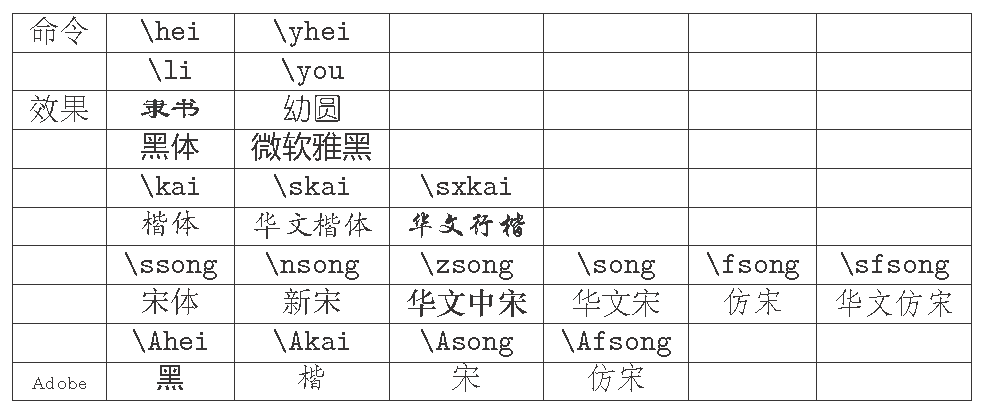
\includegraphics{figs/winfonts.png}
% \end{figure}
% \subsection{学校配色与Logo}
% \subsubsection{配色}
% 学校的配色示例文件在 \pkg{beamercolorthemeustc.sty}, 自己可以仿照配置模板
% 颜色.
% \subsubsection{Logo}
%   你可以使用 \opt{logo} 选项来在报告首页生成学校和学院的logo. 
%   学校与学院的Logo都放在 \file{logo/} 目录下. 
%   这个对不同学校而言当然是不同
%   的, 如果你要使用自己学校的logo, 请注意以下
%   \begin{itemize}
%     \item 两个logo的高度都为 \opt{1cm}, 而且都没有背景
%	格式为pdf. 请使用图像处理软件(GIMP)处理;
%     \item 图标的颜色应该和整个模板的配色协调. 故你要么更改图标的颜色,%       要么更改本模板的配色;
%     \item 最后你还需要检查背景色和前景色的配合是否具有高对比度(字体能
%	看清), 我使用的是\href{http://contrastchecker.com/}
%	{Contrast Checker}.
%   \end{itemize}
% \subsection{定理环境的使用}
% \subsubsection{自带定理环境}
% \pkg{beamer} 自身已经定义了定理环境\cite{tantau2004user}*{p.~193}: 
% \env{theorem}, \env{lemma}, \env{definition},
% \env{corollary}, \env{example}, 
% \env{proposition}(好像我不能使用 \env{proposition})
% \begin{latex}
%   \begin{theorem}[勾股定理]
%     假设$a,b,c$是直角三角形的三边, 且$c>a\geq b>0$, 则
%     \[
%	a^a+b^2=c^2.
%     \]
%   \end{theorem}
% \end{latex}
% \subsubsection{预定义定理环境}
% 除了beamer默认定义的定理环境, 本模板还自带定义了一些定理环境,
% 具体请参考配置文件: \file{ustcmb.cfg}.
%
% 这里举例如下
% \begin{latex}
%  \begin{thm}[勾股定理]
%     假设$a,b,c$是直角三角形的三边, 且$c>a\geq b>0$, 则
%     \[
%	a^a+b^2=c^2.
%     \]
%   \end{thm}
% \end{latex}
% \subsubsection{定理环境的变式}
% 定理环境有两个变式, 即 \env{Block} 与 \env{AlertBlock}. 示例如下:
% \begin{latex}
%   \begin{block}{Block Title}
%     Block示例
%   \end{block}
%   \begin{alertblock}
%     AlertBlock示例
%   \end{alertblock}
% \end{latex}
% \subsubsection{长定理的写法}
% 在实际写作中, 我们可能遇到一个定理太长, 需要分两个 \env{frame} 来写.
% 此时可以使用如下的例子来手动分页:
% \begin{latex}
%   \begin{thm}
%     长定理的内容, 超过一页
%   \end{thm}
%   \adtocounter{thm}{-1}
%   \begin{thm}[Cont.]
%     长定理超过一页的部分
%   \end{thm}
% \end{latex}
% 这里的要点是通过重置 \env{thm} 的编号来实现定理编号的正确.
% \subsection{自动分页与\env{itemize}的分步显示}
% 我们知道, 可以对\env{frame}使用选项\opt{allowframebreaks}来自动分页。
% 但是这种方法会使得分步显示无效。解决办法是使用cover:
% \begin{latex}
%   \begin{frame}[<+->]{自动分页与分步显示}
%     \begin{onlyenv}<1>
%       第一页内容
%     \end{onlyenv}
%     \begin{onlyenv}<2->
%       第二页放置一个列表
%       \begin{itemize}[<+(1)->]
%         \item 第一项
%         \item 第二项
%       \end{itemize}
%       我们应该注意到\opt{(+1)}, 它表示将暂停计数器(beamerpause)
%       加1, 从而第一项在第二帧显示, 而第二项在第3帧显示.
%     \end{onlyenv}
%   \end{frame} 
% \end{latex}
% \subsection{打印模式}
% 本模板提供了方便打印slide的模式 \opt{print}, 使用该模式会作如下改变
% \begin{itemize}
%   \item 主题颜色设置灰色, 并且带有灰度背景, 方便查看是否超出边距;
%   \item 4张幻灯片放到一页A4(横向)纸上;
%   \item 同一个frame中的多个遮罩(overlay)会合并到一页打印;
%   \item 由于默认使用的是 \opt{handout} 模式来打印, 参考文献列表不会打印.
% \end{itemize}
% \subsection{反馈}
% 非常感谢你使用本模板, 若你在使用过程中有任何疑问/建议. 
% 请不要吝啬, 将其反馈到模板
% \href{https://github.com/vanabel/mathbeamer/issues}{发布主页}.
%
% 此外你还可以加入QQ群\href{https://goo.gl/i1kcwe}{LaTeX讨论区}.
% \StopEventually{}
% \section{类文件源码}
%    \begin{macrocode}
%<*class>
%    \end{macrocode}
% \subsection{宏包依赖}
% 使用 \pkg{etoolbox} 来设置启用/禁用选项
%    \begin{macrocode}
\RequirePackage{etoolbox}
\RequirePackage{xcolor}
%    \end{macrocode}
% 数学定理与字体支持
%    \begin{macrocode}
\RequirePackage{mathtools, bm}
%    \end{macrocode}
% 英文断行
%    \begin{macrocode}
\RequirePackage[english]{babel}
%    \end{macrocode}
% 超链接
%    \begin{macrocode}
\AtBeginDocument{
  \RequirePackage{hyperref}
  \hypersetup{
    pdfpagemode=FullScreen,
    bookmarksopen=false,
    pdfencoding=auto,
    colorlinks=true,
    %ocgcolorlinks,
    %pdfusetitle
  }
}
%    \end{macrocode}
% \subsection{选项申明}
% \opt{print}选项: 编译打印版本
%    \begin{macrocode}
\providetoggle{print}
\DeclareOption{print}{\toggletrue{print}}
%    \end{macrocode}
% \opt{nds}选项: 不启用默认设置
%    \begin{macrocode}
\newif\ifMB@nds\MB@ndsfalse
\DeclareOption{nds}{\MB@ndstrue}
%    \end{macrocode}
% \opt{thmnum}选项: 定理有编号
%    \begin{macrocode}
\newif\ifMB@thmnum\MB@thmnumfalse
\DeclareOption{thmnum}{\MB@thmnumtrue}
%    \end{macrocode}
% \opt{subnav}选项:插入小节导航
%    \begin{macrocode}
\newif\ifMB@subnav\MB@subnavfalse
\DeclareOption{subnav}{\MB@subnavtrue}
%    \end{macrocode}
% \opt{eqsecnum}选项: 以节编号公式
%    \begin{macrocode}
\newif\ifMB@eqsecnum\MB@eqsecnumfalse
\DeclareOption{eqsecnum}{\MB@eqsecnumtrue}
%    \end{macrocode}
% \opt{authoryear}选项: 作者年代(bibtex)引用方式
%    \begin{macrocode}
\newif\ifMB@authoryear\MB@authoryearfalse
\DeclareOption{authoryear}{\MB@authoryeartrue}
%    \end{macrocode}
% \opt{allcite}选项: 列出所有参考文献
%    \begin{macrocode}
\newif\ifMB@allcites\MB@allcitesfalse
\DeclareOption{allcites}{\MB@allcitestrue}
%    \end{macrocode}
% \opt{nobib}选项: 去掉参考文献列表
%    \begin{macrocode}
\newif\ifMB@nobib\MB@nobibfalse
\DeclareOption{nobib}{\MB@nobibtrue}
%    \end{macrocode}
% \opt{biblatex}选项: 使用现代biblatex包替代amsrefs
%    \begin{macrocode}
\newif\ifMB@biblatex\MB@biblatexfalse
\DeclareOption{biblatex}{\MB@biblatextrue}
%    \end{macrocode}





% \opt{citemath}选项: biblatex的数学论文专用引用样式(需要xstring包)
%    \begin{macrocode}
\newif\ifMB@citemath\MB@citemathfalse
\DeclareOption{citemath}{\MB@citemathtrue}
%    \end{macrocode}

% \opt{zh}选项: 中文模式
%    \begin{macrocode}
\DeclareOption{zh}{\MB@zhtrue}
\newif\ifMB@zh\MB@zhfalse
%    \end{macrocode}
% \opt{logo}选项: 使用logo
%    \begin{macrocode}
\DeclareOption{logo}{\MB@logotrue}
\newif\ifMB@logo\MB@logofalse
%    \end{macrocode}
% 传递参数
%    \begin{macrocode}
\DeclareOption*{\PassOptionsToClass{\CurrentOption}{beamer}}
\ProcessOptions\relax
%    \end{macrocode}
% 提供标准的类声明
%    \begin{macrocode}
\ProvidesClass{ustcmb}[2025/08/21 v2.2.7 USTC Math Beamer Template]
%    \end{macrocode}
% \subsection{基于模式加载文档类}
% 如果是打印(\opt{print})模式
%    \begin{macrocode}
\iftoggle{print}{
  \LoadClass[handout, nds]{beamer}
  \RequirePackage{pgfpages}
  \pgfpagesuselayout{4 on 1}[a4paper,border shrink=5mm,landscape]
  \mode<handout>{\setbeamercolor{background canvas}{bg=black!5}}
}
%    \end{macrocode}
% 否则是报告模式, 生成报告
%    \begin{macrocode}
{
  \LoadClass{beamer}
}
%    \end{macrocode}
% \subsection{选项实现}
% \opt{zh}选项: 表示使用中文模式
%    \begin{macrocode}
\ifMB@zh
%    \end{macrocode}
% ctex 中文支持引擎
%    \begin{macrocode}
\RequirePackage{ctex}
%    \end{macrocode}
%% 中文模式下字体配置, 主要更改了标题(title)/帧标题(frametitle)/正文(normal text). 其他结构的修改可以参考\href{http://www.cpt.univ-mrs.fr/~masson/latex/Beamer-appearance-cheat-sheet.pdf}{Beamer appearance cheat sheet}.
%    \begin{macrocode}
\ifMB@zh
\setbeamerfont*{title}{family=\sffamily, shape=\scshape, series=\bfseries, size=\LARGE}
\setbeamerfont{frametitle}{family=\sffamily, shape=\upshape, series=\bfseries}
\setbeamerfont{normal text}{family=\rmfamily, shape=\upshape, series=\mdseries}
\AtBeginDocument{\usebeamerfont{normal text}}
\fi
%    \end{macrocode}
%% 中文强调
%    \begin{macrocode}
\RequirePackage{ulem}
\AtEndOfClass{% ^^A documentation part start with %
% ^^A All other parts are called definition parts
% ^^A Comments in documentation part
% ^^A equivalently use \iffalse ... \fi
% \iffalse meta-comment
% !TeX program = XeLaTeX
% !TeX encoding = UTF-8

% This work may be distributed and/or modified under the
% conditions of the LaTeX Project Public License, either
% version 1.3c of this license or (at your option) any later
% version. This version of this license is in
%    http://www.latex-project.org/lppl/lppl-1-3c.txt
% and the latest version of this license is in
%    http://www.latex-project.org/lppl.txt
% and version 1.3 or later is part of all distributions of
% LaTeX version 2005/12/01 or later.
%
% This work has the LPPL maintenance status `maintained'.
%
% The Current Maintainers of this work is Van Abel.
%
% ---------------------------------------------------------------------
%
%<*internal>
\iffalse
%</internal>
%<*readme>
# ustcmb --- 数学类报告模板

[![License](https://img.shields.io/badge/License-LPPL%20v1.3c-blue.svg)](http://www.latex-project.org/lppl.txt)
[![Version](https://img.shields.io/badge/Version-v2.2.4-green.svg)](https://github.com/vanabel/mathbeamer)
[![LaTeX](https://img.shields.io/badge/LaTeX-Beamer-orange.svg)](https://www.ctan.org/pkg/beamer)

> 基于USTC学校主题定制的数学报告模板,支持中英文双语,提供良好的打印模式

## 📖 简介

`ustcmb` (ustcmethbeamer) 是基于USTC学校主题定制的报告模板,利用它可以非常方便地制作数学类幻灯片。它同时支持中文与英文的处理,以及良好的打印模式。

### ✨ 主要特性

- 🎨 基于USTC学校主题的现代化设计
- 🌏 完整的中英文双语支持
- 📚 灵活的参考文献处理(支持amsrefs和biblatex)
- 🎯 丰富的定理环境配置选项
- 🖨️ 优化的打印模式支持
- 📱 响应式布局设计

## 🚀 快速开始

### 下载安装

1. 下载模板压缩包:[最新版本](https://github.com/vanabel/mathbeamer/releases/latest)
2. 解压后阅读示例文件 `ustcmb-main.pdf`
3. 参考 `ustcmb-main.tex` 开始编写您的报告

### 基本使用

```latex
\documentclass[zh]{ustcmb}

\title{您的报告标题}
\author{您的姓名}
\institute{您的机构}

\begin{document}
\frame{\titlepage}

\begin{frame}
\frametitle{第一张幻灯片}
内容...
\end{frame}

\end{document}
```

## ⚙️ 配置选项

### 核心选项

| 选项 | 描述 | 默认值 |
|------|------|--------|
| `zh` | 启用中文支持 | 启用 |
| `en` | 英文模式 | 禁用 |
| `thmnum` | 定理带编号 | 禁用 |
| `eqsecnum` | 公式以节编号 | 禁用 |

### 参考文献选项

| 选项 | 描述 | 依赖 |
|------|------|------|
| `authoryear` | 作者年代引用样式 (amsrefs) | amsrefs |
| `allcites` | 输出bib.bib中的所有参考文献 | amsrefs |
| `biblatex` | 使用现代biblatex包 | biblatex |
| `citemath` | 数学论文专用引用样式 | biblatex + xstring |

### 高级选项

| 选项 | 描述 |
|------|------|
| `nds` | 不使用默认设置(需要手动配置) |
| `subnav` | 在每个子节显示导航 |
| `nobib` | 禁用参考文献处理 |

## 📚 示例文件

项目包含多个示例文件,帮助您快速上手:

- `ustcmb-main.tex` - 主要示例文件
- `biblatex-example.tex` - biblatex使用示例
- `amsrefs-example.tex` - amsrefs使用示例
- `math-citation-example.tex` - 数学引用示例

## 🔧 自定义配置

### 使用nds选项时的必要配置

当使用 `nds` 选项时,您需要手动配置以下内容:

```latex
\documentclass[nds]{ustcmb}

% 设置主题
\usetheme{YourTheme}

% 设置标题页
\begin{document}
\frame{\titlepage}

% 设置定理环境
\newtheorem{thm}{Theorem}

% 可选:设置颜色主题
\usecolortheme{YourColorTheme}
```

### 字体配置

模板支持自定义中文字体:

```latex
% 在导言区设置
\setCJKmainfont{YourChineseFont}
\setCJKsansfont{YourChineseSansFont}
```

## 📋 版本历史

### [v2.2.4] (开发中)

- ✨ 新增 `biblatex` 选项,支持现代参考文献处理
- ✨ 新增多种引用样式选项
- 🔄 保持对传统 `amsrefs` 的向后兼容性
- ⚡ 优化参考文献配置和引用格式

### [v2.2.3]

- ✨ 新增 `nobib` 选项
- 🧹 移除多余的参考文献导航
- 🔤 重新设置中文字体,支持Mac和Windows系统
- 🎨 重新配置模板标题/正文字体

### [v2.2.2]

- ✨ 新增中文自定义字体命令

### [v2.2.1]

- 🐛 修复 `\CJKunderwave` 兼容性问题

### [v2.2.0]

- ✨ 新增 `subnav` 选项:在每个子节显示导航
- 📖 添加解决 `allowframebreaks` 和 `itemize` 环境冲突的示例
- 🗑️ 移除"Thanks!"页面,应由演示总结替代

### [v2.1.0]

- 🏫 新增SJTU标志支持
- ✨ 为SJTU添加 `domc` 选项

### [v2.0.1]

- 📚 新增用户FAQ
- 🌏 根据 `zh` 或 `en` 模式修改最后一帧的感谢内容

### [v2.0.0]

- 🔧 使用dtx管理文档
- 🗑️ 移除xeCJK字体设置(应由用户自行配置)

### [v1.2.0]

- 🌏 新增中文支持选项,使用 `zh` 启用中文支持
- 🎨 新增默认颜色主题,更接近USTC颜色(主色调为蓝色)

### [v 1.1.1]

1. add more example slides, which includes
 * auto pause in lists
 * two columns in a frame
 * include figure/subfigures in a frame
 * table
 * definition/example/theorem like environments
 * custom defn/examp/thm theorem like environments
 * hyperlinks between slides
2. add thanks before the references
3. user defined commands/environments should be written in `slides/usrdefn.tex`

#### [v 1.1.0]

1. new branch, add three color style:
 * `dark`: dark color style
 * `light`: light color style
 * the default is betwen the above two

#### [v 1.0.1]

1. add link to `slides/bib.bib`, so that you can open it in `WinEdt` by `Build Tree`
2. set the default font theme for math be `\usefonttheme{professionalfonts}`, which makes math formula looks more perfect
3. add `\newcommand{}{}` example and `\newtheorem{}{}` example

### Copyright and Licence

Copyright (C) 2016 by Van Abel <van141.abel@gmail.com>

This work may be distributed and/or modified under the
conditions of the LaTeX Project Public License, either version 1.3
of this license or (at your option) any later version.
The latest version of this license is in

http://www.latex-project.org/lppl.txt

and version 1.3 or later is part of all distributions of LaTeX
version 2005/12/01 or later.

    This work consists of the file: ustcmb.dtx 
             and the derived files: ustcmb.ins
                                    ustcmb.cls
                                    ustcmb.tex
                                    ustcmb.cfg
                                    beamercolorthemeustc.sty
                                    READEME.md (this file)
%</readme>
%<*internal>
\fi    
\def\nameoflatex{plain}
\ifx\nameoflatex\fmtname\else
  \expandafter\begingroup
\fi
%</internal>
%
%<*install>

\input docstrip.tex
\keepsilent

\preamble
----------------------------------------------------------------
    模板名称: ustcmb 
        描述: 中科大数学报告模板
    模板网址: https://github.com/vanabel/mathbeamer
      版本号: v2.2.3
        作者: Van Abel
      E-mail: van141.abel@gmail.com
     License: LaTeX Project Public License v1.3c or later
 License URI: http://www.latex-project.org/lppl.txt
----------------------------------------------------------------

\endpreamble
\postamble

This is a generated file

Copyright (C) 2016 by Van Abel <van141.abel@gmail.com>

This work may be distributed and/or modified under the
conditions of the LaTeX Project Public License, either version 1.3
of this license or (at your option) any later version.
The latest version of this license is in

http://www.latex-project.org/lppl.txt

and version 1.3 or later is part of all distributions of LaTeX
version 2005/12/01 or later.

This work consists of the file ustcmb.dtx
and the derived files:
  ustcmb.ins
  ustcmb.cls
  ustcmb.tex
  ustcmb.cfg
  beamercolorthemeustc.sty

\endpostamble
\askforoverwritefalse
\generate{
  \usedir{tex/latex/ustcmb}
  \file{\jobname.cls}{\from{\jobname.dtx}{class}}
  \file{\jobname.cfg}{\from{\jobname.dtx}{cfg}}
  \file{beamercolorthemeustc.sty}{\from{\jobname.dtx}{ustc}}
  \nopreamble\nopostamble
  \usedir{doc/latex/ustcmb}
  \file{\jobname-main.tex}{\from{\jobname.dtx}{main}}
}
\obeyspaces
\Msg{****************************************************}
\Msg{*                                                   }
\Msg{* To finish the installation you have to move the   }
\Msg{* following file into a directory searched by TeX   }
\Msg{* e.g. tex/latex/ustcmb:                            }
\Msg{*                                                   }
\Msg{* \jobname.cls                                      }
\Msg{* \jobname.cfg                                      }
\Msg{* beamercolorthemeustc.sty                          }
\Msg{*                                                   }
\Msg{* To produce the documentation run the file         }
\Msg{* \jobname.dtx through XeLaTeX.                     }
\Msg{*                                                   }
\Msg{* To produce the sample file run the file           }
\Msg{* \jobname-main.tex through XeLaTeX and BibTeX      }
\Msg{*                                                   }
\Msg{* Happy TeXing!                                     }
\Msg{*                                                   }
\Msg{****************************************************}
%</install>
%<install>\endbatchfile
%
%<*internal>
\usedir{source/latex/ustcmb}
\generate{
  \file{\jobname.ins}{\from{\jobname.dtx}{install}}
}
% ^^A No extra text add by DocStrip
\nopreamble\nopostamble
\usedir{doc/latex/ustcmb}
\generate{
  \file{README.md}{\from{\jobname.dtx}{readme}}
}
% ^^A if xetex then end process of DocStrip by \endbatchfile
\ifx\nameoflatex\fmtname
  \expandafter\endbatchfile
\else
% ^^A for xelatex we close the group
  \expandafter\endgroup
\fi
%</internal>
%
%<*driver>
\ProvidesFile{\jobname.dtx}
%</driver>
%<class>\NeedsTeXFormat{LaTeX2e}[2005/12/01]
%<class>\ProvidesClass{ustcmb}
%<*class>
[2025/08/21 v2.2.4 中科大数学报告模板类文件]
%</class>
%
%<*driver>
\documentclass{ltxdoc}
\usepackage{xeCJK}
\setCJKmainfont[AutoFakeBold, ItalicFont=STKaiti]{STSong}
\setCJKsansfont[AutoFakeBold, AutoFakeSlant]{STXihei}
\setCJKmonofont[AutoFakeBold, AutoFakeSlant]{STFangsong}
\setlength\parindent{0pt}
\usepackage{booktabs,tabularx}
\usepackage{metalogo}
\usepackage{hypdoc}
\hypersetup{
  bookmarksopen=true,
  bookmarksopenlevel=2,
  bookmarksnumbered=true,
  CJKbookmarks=true,
  unicode=true,
  allcolors=blue,
}
\usepackage{xcolor} % use lightgray
\usepackage[alphabetic, msc-links, lite, abbrev]{amsrefs}
\usepackage{listings}
\lstdefinestyle{lstshell}{
  basicstyle=\small\ttfamily,
  backgroundcolor=\color{red!75!black},
  gobble=2,% 重要!否则会生成注释符号"%"
language=bash}
\lstdefinestyle{lstlatex}{
  basicstyle=\small\ttfamily,
  frame=single,
  gobble=2,
language=[LaTeX]TeX}
\lstnewenvironment{shell}{\lstset{style=lstshell}}{}
\lstnewenvironment{latex}{\lstset{style=lstlatex}}{}
\newcommand\shellcmd[1]{ \underline{\texttt{#1}}}
\EnableCrossrefs
\CodelineIndex
%\OnlyDescription
% 模仿 l3doc 的定义
\DeclareRobustCommand\file{\nolinkurl}
\DeclareRobustCommand\env{\texttt}
\DeclareRobustCommand\pkg{\textsf}
\DeclareRobustCommand\cls{\textsf}
\DeclareRobustCommand\opt{\textbf}

\renewcommand\indexname{命令索引}
\IndexPrologue{%
  \section*{\indexname}
  \textit{斜体的数字表示描述对应索引项的页码;
    带下划线的数字表示定义对应索引项的代码行号;
  罗马字体的数字表示使用对应索引项的代码行号。}
}
\RecordChanges
\def\glossaryname{版本历史}
\GlossaryPrologue{\section*{\glossaryname}}

\begin{document}
\DocInput{\jobname.dtx}
\renewcommand{\refname}{参考文献}
\begin{thebibliography}{9}
\bibitem{tantau2004user} 
Tantau, Till.
\textit{User's Guide to the Beamer Class, Version 3.01}. 
2004
\bibitem{xecjk2016manual}
CTEX.ORG.
\textit{xeCJK宏包手册}.
2006
\end{thebibliography}
\PrintChanges
\PrintIndex
\end{document}
%</driver>
% \fi
%
%
% \CharacterTable
%  {Upper-case    \A\B\C\D\E\F\G\H\I\J\K\L\M\N\O\P\Q\R\S\T\U\V\W\X\Y\Z
%   Lower-case    \a\b\c\d\e\f\g\h\i\j\k\l\m\n\o\p\q\r\s\t\u\v\w\x\y\z
%   Digits        \0\1\2\3\4\5\6\7\8\9
%   Exclamation   \!     Double quote  \"     Hash (number) \#
%   Dollar        \$     Percent       \%     Ampersand     \&
%   Acute accent  \'     Left paren    \(     Right paren   \)
%   Asterisk      \*     Plus          \+     Comma         \,
%   Minus         \-     Point         \.     Solidus       \/
%   Colon         \:     Semicolon     \;     Less than     \<
%   Equals        \=     Greater than  \>     Question mark \?
%   Commercial at \@     Left bracket  \[     Backslash     \\
%   Right bracket \]     Circumflex    \^     Underscore    \_
%   Grave accent  \`     Left brace    \{     Vertical bar  \|
%   Right brace   \}     Tilde         \~}
% \changes{v2.2.4}{2025/08/21}{新增\opt{biblatex}选项,支持现代参考文献处理}
% \changes{v2.2.4}{2025/08/21}{新增\opt{citemath}选项,支持数学论文专用引用样式}
% \changes{v2.2.4}{2025/08/21}{保持对传统\pkg{amsrefs}的向后兼容性}
% \changes{v2.2.4}{2025/08/21}{优化参考文献配置和引用格式}
% \changes{v2.2.3}{2018/06/03}{移除多余的参考文献导航}
% \changes{v2.2.3}{2018/06/03}{重新设置中文字体,使得Mac系统和Windows系统都可用}
% \changes{v2.2.3}{2018/06/03}{新增\shellcmd{nobib}选项}
% \changes{v2.2.2}{2018/06/02}{新增中文字体命令}
% \changes{v2.2.1}{2018/04/05}{修复\env{CJKunderwave}的不兼容性}
% \changes{v2.2.0}{2017/11/29}{新增小节导航选项\opt{subnav}}
% \changes{v2.2.0}{2017/11/29}{新增示例:\opt{allowframebreaks}与\env{itemize}分步显示}
% \changes{v2.2.0}{2017/11/29}{移出致谢页,因为在报告结束应该呈现一个你报告主题的摘要而非简单的``谢谢''两个字}
% \changes{v2.1.0}{2017/11/07}{新增上海交大学院与学校logo}
% \changes{v2.1.0}{2017/11/07}{新增用户快速配色, 只需改变主配色\shellcmd{domc}的值, 详见示例文档\file{math-beamer.tex}}
% \changes{v2.0.1}{2017/04/30}{提供用户使用FAQ}
% \changes{v2.0.1}{2017/04/30}{修改致谢/Thanks以匹配语言}
% \changes{v2.0.0}{2016/12/14}{使用dtx管理文档}
% \changes{v1.2.0}{2016/05/15}{Add chinese support option, just use `zh` to support chinese}
% \changes{v1.2.0}{2016/05/15}{Add default colortheme to be more like USTC color (blue in main)}
% \changes{v1.1.1}{2015/09/21}{Add more example slides}
% \changes{v1.1.1}{2015/09/21}{Add thanks before the references}
% \changes{v1.1.1}{2015/09/21}{Add user-defined commands/environments in \file{slides/usrdefn.tex}}
% \changes{v1.1.0}{2015/09/20}{New branch, add three color style}
% \changes{v1.0.1}{2015/09/20}{Add links supported by WinEdt Build Tree to \file{slides/bib.bib}}
% \changes{v1.0.1}{2015/09/20}{Add |newcommand| and |newtheorem| examples}
% \changes{v1.0.0}{2015/09/19}{Initial version}

% \GetFileInfo{\jobname.dtx}
%
% \DoNotIndex{\%,\#,\$,\%,\&,\@,\\,\{,\},\^,\_,\~,\ ,\[,\],\documentclass}
% \DoNotIndex{\@ne,\and,\author,\centerline,\date,\inst,\institute}
% \DoNotIndex{\definecolor,\decumentclass,\label,\newtheorem,\sc}
% \DoNotIndex{\setbeamercolor,\setbeamercovered,\setbeamertemplate}
% \DoNotIndex{\cite,\uwave,\cline,\eps,\epsilon,\geq}
% \DoNotIndex{\hline,\href,\item,\jobname,\lipsum,\lstinline}
% \DoNotIndex{\lstset,\small,\subsection,\textwidth,\ttfamily}
% \DoNotIndex{\tableofcontents, \setCJKmainfont,\setbeamerfont}
% \DoNotIndex{\setCJKmonofont,\setCJKsansfont,\subject,\subtitle}
% \DoNotIndex{\theoremstyle, \title, \titlepage, \usepackage}
% \DoNotIndex{\advance,\begingroup,\catcode,\closein}
% \DoNotIndex{\closeout,\day,\def,\edef,\else,\empty,\endgroup}
% \DoNotIndex{\addtobeamertemplate, \addtocounter}
% \DoNotIndex{\AtBeginDocument,\AtEndDocument,\AtEndOfClass}
% \DoNotIndex{\begin,\end,\bfseries,\bibliography}
% \DoNotIndex{\color,\CurrentOption,\DeclareOption,\fi,\frame}
% \DoNotIndex{\hfill,\hypersetup,\iftoggle,\includegraphics,\input}
% \DoNotIndex{\insertframenumber,\inserttotalframenumber}
% \DoNotIndex{\mode,\LARGE,\LoadClass,\necounter,\noewif,\nocite}
% \DoNotIndex{\numberwithin,\PassOptionsToClass,\pgfpagesuselayout}
% \DoNotIndex{\ProcessOptions, \providetoggle,\relax,\renewcommand}
% \DoNotIndex{\RequirePackage, \section, \setcounter, \toggletrue}
% \DoNotIndex{\value,\newcommand,\newif,\newcounter}
% \DoNotIndex{\ccwd,\caption,\captionsetup,\chapter,\ctexset}
% \DoNotIndex{\itemsep,\hangindent,\setfontsize,\setlength,\hdclindex}
% \DoNotIndex{\textbf,\newenvironment,\newcommand}
% \DoNotIndex{\n,\newCJKfontfamily,\AtBeginSubsection}
% \expandafter\DoNotIndex\expandafter{\string\&}
%
% \title{\textsf{ustcmb}类用户手册\thanks{这是
%   \textsf{ustcmb}~\fileversion 的用户使用说明文档,
%   创建于 \filedate.}}
% \author{Van Abel \\ \texttt{\small van141.abel@gmail.com}}
% \date{\filedate}
%
% \maketitle
% \def\abstractname{摘要}
% \begin{abstract}
%   \cls{ustcmb}是我准备博士论文答辩时制作的模板. 它主要是为了方便数学
%   专业的同学写报告. 其中定义了几个选项方便快速实现功能定制, 而且还配
%   置了与USTC学校主页相适配的主题以及显示学校/学院Logo.
%
%   \cls{ustcmb.cls}文档类只支持\XeLaTeX{}方式编译. 模板提供了示例文件 \file{\jobname-main.tex}以及配色文件 \pkg{beamercolorthemeustc.sty}.
% \end{abstract}
% 
% \section{简介}
% 
%   本报告模板旨在方便大家轻松上手制作报告. 在一定程度上定制报告格式,
%   应大家要求还同时支持中文和英文. 支持选项如下:
% \begin{table}[htbp]
%   \begin{tabular}{|l|p{.75\textwidth}|}
%     \hline
%     \opt{zh} & 中文支持(ctex) \\
%     \hline
%     \opt{logo} & 使用学校以及学院Logo \\
%     \hline
%     \opt{thmnum} & 定理编号\\
%     \hline
%     \opt{eqsecnum} & 公式以节编号\\
%     \hline
%     \opt{subnav} & 在每小节开始显示小节导航\\
%     \hline
%     \opt{authoryear} & 作者年代型文献引用(amsrefs)\\
%     \hline
%     \opt{allcites} & 自动列出所有参考文献\\
%     \hline
%     \opt{biblatex} & 使用现代biblatex包替代amsrefs\\
%     \hline

%     \hline


%     \opt{citemath} & biblatex数学论文专用引用样式(需要xstring包)\\
%     \hline
%     \opt{nds} & 不使用默认设置\\
%     \hline
%     \opt{nobib} & 不列出参考文献\\
%     \hline
%     \opt{print} & 打印模式\\
%     \hline
%   \end{tabular}
% \end{table}
% \section{模板生成与安装} 
% 本发行版已经包含所有的生成文件. 所以, 如果您对如何生成模板文件
% 不感兴趣, 则完全可以跳过这一节.
% 
% 模板解压缩后生成文件夹 \file{ustcmb-vN.M}, 其中 \file{vN.M} 为版本号. 
% 该文件夹包含以下文件
% \begin{itemize}
%  \item \file{ustcmb.dtx}: 模板文档源文件
%  \item \file{ustcmb.tex}: 模板示例文件
%  \item \cls{ustcmb.cls}: 模板类文件
%  \item \file{ustcmb.cfg}: 英文/中文定理配置文件
%  \item \pkg{beamercolorthemeustc.sty}: 模板配色文件
% \end{itemize}
% Linux/Mac用户可以直接使用 GNU make 工具, 
% Windows用户建议安装 \href{https://www.cygwin.com/}{Cygwin}
% 然后同样使用 GUN make 工具.
% \begin{itemize}
%  \item 编译文档\shellcmd{make doc}
%  \item 编译示例文件\shellcmd{make main}
%  \item 安装模板到TeX系统\shellcmd{make inst}
%  \item 以管理员方式安装模板到TeX系统\shellcmd{make install}
%  \item 从TeX系统卸载模板\shellcmd{make uninst}
%  \item 以管理员方式从TeX系统卸载模板\shellcmd{make uninstall}
%  \item 清空临时文件\shellcmd{make clean}
%  \item 清空所有生成文件\shellcmd{make distclean}
%  \item 打包文件以发布\shellcmd{make zip}
% \end{itemize}
% \section{使用手册}
% 这节主要讲一讲支持的选项. 
% \subsection{中文支持}
% 中文采用的是 \pkg{ctex} 方案, 使用时只需添加 \opt{zh} 选项即可.
% 
% 需要注意的是, 默认状态下\texttt{并没有配置任何中文字体}. 
% 故可能产生以下问题:
% \begin{itemize}
%   \item 在旧版本的\pkg{xeCJK} 中编译不通过(因为没有默认配置字体). 
%     此时需要升级 \pkg{xeCJK} 包即可.
%   \item \pkg{xeCJK} 默认的字体是黑体, 也许不适用于正式场合. 
%   \item 如何查看以及使用字体, 请参考\cite[p.~8, 3.2.1节]
%     {xecjk2016manual}. 例如你可以在导言区加入
%   \begin{latex}	    
%     \setCJKmainfont[AutoFakeSlant, AutoFakeBold]{SimSun}
%     \setCJKmonofont[AutoFakeSlant, AutoFakeBold]{FangSong}
%     \setCJKsansfont[AutoFakeSlant, AutoFakeBold]{KaiTi}
%   \end{latex}
%   如果你要使用黑体为正文字体,只需将上述命令修改为
%   \begin{latex}
%     \setCJKmainfont[AutoFakeSlant, AutoFakeBold]{SimHei}
%   \end{latex}
% \end{itemize}
% 此外,在v2.2.2版中,还增加了一些默认的字体命令,但是这些字体默认都没有启用,要使用这些字体命令,
% 请进行如下操作:
% \begin{enumerate}
%   \item 打开根目录下的\file{ustcmb.cfg}, 去掉你想要使用的字体前的两个百分号,例如
%     \begin{latex}
% %%  微软雅黑
% %%  \newCJKfontfamily[yhei]\yhei{Microsoft YaHei}
%     \end{latex}
%   \item 在\file{ustcmb-main.tex}的正文中使用(当然你得确保系统由微软雅黑字体)
%     \begin{latex}
% 正文{\yhei 这是雅黑}正文
%     \end{latex}
% \end{enumerate}
% \begin{figure}[htbp]
%   \centering
%   \caption{完整的字体列表与效果}
%   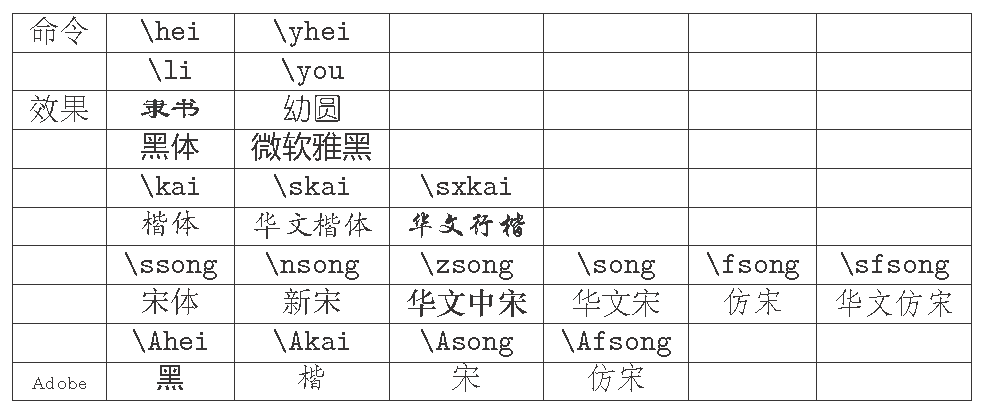
\includegraphics{figs/winfonts.png}
% \end{figure}
% \subsection{学校配色与Logo}
% \subsubsection{配色}
% 学校的配色示例文件在 \pkg{beamercolorthemeustc.sty}, 自己可以仿照配置模板
% 颜色.
% \subsubsection{Logo}
%   你可以使用 \opt{logo} 选项来在报告首页生成学校和学院的logo. 
%   学校与学院的Logo都放在 \file{logo/} 目录下. 
%   这个对不同学校而言当然是不同
%   的, 如果你要使用自己学校的logo, 请注意以下
%   \begin{itemize}
%     \item 两个logo的高度都为 \opt{1cm}, 而且都没有背景
%	格式为pdf. 请使用图像处理软件(GIMP)处理;
%     \item 图标的颜色应该和整个模板的配色协调. 故你要么更改图标的颜色,%       要么更改本模板的配色;
%     \item 最后你还需要检查背景色和前景色的配合是否具有高对比度(字体能
%	看清), 我使用的是\href{http://contrastchecker.com/}
%	{Contrast Checker}.
%   \end{itemize}
% \subsection{定理环境的使用}
% \subsubsection{自带定理环境}
% \pkg{beamer} 自身已经定义了定理环境\cite{tantau2004user}*{p.~193}: 
% \env{theorem}, \env{lemma}, \env{definition},
% \env{corollary}, \env{example}, 
% \env{proposition}(好像我不能使用 \env{proposition})
% \begin{latex}
%   \begin{theorem}[勾股定理]
%     假设$a,b,c$是直角三角形的三边, 且$c>a\geq b>0$, 则
%     \[
%	a^a+b^2=c^2.
%     \]
%   \end{theorem}
% \end{latex}
% \subsubsection{预定义定理环境}
% 除了beamer默认定义的定理环境, 本模板还自带定义了一些定理环境,
% 具体请参考配置文件: \file{ustcmb.cfg}.
%
% 这里举例如下
% \begin{latex}
%  \begin{thm}[勾股定理]
%     假设$a,b,c$是直角三角形的三边, 且$c>a\geq b>0$, 则
%     \[
%	a^a+b^2=c^2.
%     \]
%   \end{thm}
% \end{latex}
% \subsubsection{定理环境的变式}
% 定理环境有两个变式, 即 \env{Block} 与 \env{AlertBlock}. 示例如下:
% \begin{latex}
%   \begin{block}{Block Title}
%     Block示例
%   \end{block}
%   \begin{alertblock}
%     AlertBlock示例
%   \end{alertblock}
% \end{latex}
% \subsubsection{长定理的写法}
% 在实际写作中, 我们可能遇到一个定理太长, 需要分两个 \env{frame} 来写.
% 此时可以使用如下的例子来手动分页:
% \begin{latex}
%   \begin{thm}
%     长定理的内容, 超过一页
%   \end{thm}
%   \adtocounter{thm}{-1}
%   \begin{thm}[Cont.]
%     长定理超过一页的部分
%   \end{thm}
% \end{latex}
% 这里的要点是通过重置 \env{thm} 的编号来实现定理编号的正确.
% \subsection{自动分页与\env{itemize}的分步显示}
% 我们知道, 可以对\env{frame}使用选项\opt{allowframebreaks}来自动分页。
% 但是这种方法会使得分步显示无效。解决办法是使用cover:
% \begin{latex}
%   \begin{frame}[<+->]{自动分页与分步显示}
%     \begin{onlyenv}<1>
%       第一页内容
%     \end{onlyenv}
%     \begin{onlyenv}<2->
%       第二页放置一个列表
%       \begin{itemize}[<+(1)->]
%         \item 第一项
%         \item 第二项
%       \end{itemize}
%       我们应该注意到\opt{(+1)}, 它表示将暂停计数器(beamerpause)
%       加1, 从而第一项在第二帧显示, 而第二项在第3帧显示.
%     \end{onlyenv}
%   \end{frame} 
% \end{latex}
% \subsection{打印模式}
% 本模板提供了方便打印slide的模式 \opt{print}, 使用该模式会作如下改变
% \begin{itemize}
%   \item 主题颜色设置灰色, 并且带有灰度背景, 方便查看是否超出边距;
%   \item 4张幻灯片放到一页A4(横向)纸上;
%   \item 同一个frame中的多个遮罩(overlay)会合并到一页打印;
%   \item 由于默认使用的是 \opt{handout} 模式来打印, 参考文献列表不会打印.
% \end{itemize}
% \subsection{反馈}
% 非常感谢你使用本模板, 若你在使用过程中有任何疑问/建议. 
% 请不要吝啬, 将其反馈到模板
% \href{https://github.com/vanabel/mathbeamer/issues}{发布主页}.
%
% 此外你还可以加入QQ群\href{https://goo.gl/i1kcwe}{LaTeX讨论区}.
% \StopEventually{}
% \section{类文件源码}
%    \begin{macrocode}
%<*class>
%    \end{macrocode}
% \subsection{宏包依赖}
% 使用 \pkg{etoolbox} 来设置启用/禁用选项
%    \begin{macrocode}
\RequirePackage{etoolbox}
\RequirePackage{xcolor}
%    \end{macrocode}
% 数学定理与字体支持
%    \begin{macrocode}
\RequirePackage{mathtools, bm}
%    \end{macrocode}
% 英文断行
%    \begin{macrocode}
\RequirePackage[english]{babel}
%    \end{macrocode}
% 超链接
%    \begin{macrocode}
\AtBeginDocument{
  \RequirePackage{hyperref}
  \hypersetup{
    pdfpagemode=FullScreen,
    bookmarksopen=false,
    pdfencoding=auto,
    colorlinks=true,
    %ocgcolorlinks,
    %pdfusetitle
  }
}
%    \end{macrocode}
% \subsection{选项申明}
% \opt{print}选项: 编译打印版本
%    \begin{macrocode}
\providetoggle{print}
\DeclareOption{print}{\toggletrue{print}}
%    \end{macrocode}
% \opt{nds}选项: 不启用默认设置
%    \begin{macrocode}
\newif\ifMB@nds\MB@ndsfalse
\DeclareOption{nds}{\MB@ndstrue}
%    \end{macrocode}
% \opt{thmnum}选项: 定理有编号
%    \begin{macrocode}
\newif\ifMB@thmnum\MB@thmnumfalse
\DeclareOption{thmnum}{\MB@thmnumtrue}
%    \end{macrocode}
% \opt{subnav}选项:插入小节导航
%    \begin{macrocode}
\newif\ifMB@subnav\MB@subnavfalse
\DeclareOption{subnav}{\MB@subnavtrue}
%    \end{macrocode}
% \opt{eqsecnum}选项: 以节编号公式
%    \begin{macrocode}
\newif\ifMB@eqsecnum\MB@eqsecnumfalse
\DeclareOption{eqsecnum}{\MB@eqsecnumtrue}
%    \end{macrocode}
% \opt{authoryear}选项: 作者年代(bibtex)引用方式
%    \begin{macrocode}
\newif\ifMB@authoryear\MB@authoryearfalse
\DeclareOption{authoryear}{\MB@authoryeartrue}
%    \end{macrocode}
% \opt{allcite}选项: 列出所有参考文献
%    \begin{macrocode}
\newif\ifMB@allcites\MB@allcitesfalse
\DeclareOption{allcites}{\MB@allcitestrue}
%    \end{macrocode}
% \opt{nobib}选项: 去掉参考文献列表
%    \begin{macrocode}
\newif\ifMB@nobib\MB@nobibfalse
\DeclareOption{nobib}{\MB@nobibtrue}
%    \end{macrocode}
% \opt{biblatex}选项: 使用现代biblatex包替代amsrefs
%    \begin{macrocode}
\newif\ifMB@biblatex\MB@biblatexfalse
\DeclareOption{biblatex}{\MB@biblatextrue}
%    \end{macrocode}





% \opt{citemath}选项: biblatex的数学论文专用引用样式(需要xstring包)
%    \begin{macrocode}
\newif\ifMB@citemath\MB@citemathfalse
\DeclareOption{citemath}{\MB@citemathtrue}
%    \end{macrocode}

% \opt{zh}选项: 中文模式
%    \begin{macrocode}
\DeclareOption{zh}{\MB@zhtrue}
\newif\ifMB@zh\MB@zhfalse
%    \end{macrocode}
% \opt{logo}选项: 使用logo
%    \begin{macrocode}
\DeclareOption{logo}{\MB@logotrue}
\newif\ifMB@logo\MB@logofalse
%    \end{macrocode}
% 传递参数
%    \begin{macrocode}
\DeclareOption*{\PassOptionsToClass{\CurrentOption}{beamer}}
\ProcessOptions\relax
%    \end{macrocode}
% 提供标准的类声明
%    \begin{macrocode}
\ProvidesClass{ustcmb}[2025/08/21 v2.2.5 USTC Math Beamer Template]
%    \end{macrocode}
% \subsection{基于模式加载文档类}
% 如果是打印(\opt{print})模式
%    \begin{macrocode}
\iftoggle{print}{
  \LoadClass[handout, nds]{beamer}
  \RequirePackage{pgfpages}
  \pgfpagesuselayout{4 on 1}[a4paper,border shrink=5mm,landscape]
  \mode<handout>{\setbeamercolor{background canvas}{bg=black!5}}
}
%    \end{macrocode}
% 否则是报告模式, 生成报告
%    \begin{macrocode}
{
  \LoadClass{beamer}
}
%    \end{macrocode}
% \subsection{选项实现}
% \opt{zh}选项: 表示使用中文模式
%    \begin{macrocode}
\ifMB@zh
%    \end{macrocode}
% ctex 中文支持引擎
%    \begin{macrocode}
\RequirePackage{ctex}
%    \end{macrocode}
%% 中文模式下字体配置, 主要更改了标题(title)/帧标题(frametitle)/正文(normal text). 其他结构的修改可以参考\href{http://www.cpt.univ-mrs.fr/~masson/latex/Beamer-appearance-cheat-sheet.pdf}{Beamer appearance cheat sheet}.
%    \begin{macrocode}
\ifMB@zh
\setbeamerfont*{title}{family=\sffamily, shape=\scshape, series=\bfseries, size=\LARGE}
\setbeamerfont{frametitle}{family=\sffamily, shape=\upshape, series=\bfseries}
\setbeamerfont{normal text}{family=\rmfamily, shape=\upshape, series=\mdseries}
\AtBeginDocument{\usebeamerfont{normal text}}
\fi
%    \end{macrocode}
%% 中文强调
%    \begin{macrocode}
\RequirePackage{ulem}
\AtEndOfClass{% ^^A documentation part start with %
% ^^A All other parts are called definition parts
% ^^A Comments in documentation part
% ^^A equivalently use \iffalse ... \fi
% \iffalse meta-comment
% !TeX program = XeLaTeX
% !TeX encoding = UTF-8

% This work may be distributed and/or modified under the
% conditions of the LaTeX Project Public License, either
% version 1.3c of this license or (at your option) any later
% version. This version of this license is in
%    http://www.latex-project.org/lppl/lppl-1-3c.txt
% and the latest version of this license is in
%    http://www.latex-project.org/lppl.txt
% and version 1.3 or later is part of all distributions of
% LaTeX version 2005/12/01 or later.
%
% This work has the LPPL maintenance status `maintained'.
%
% The Current Maintainers of this work is Van Abel.
%
% ---------------------------------------------------------------------
%
%<*internal>
\iffalse
%</internal>
%<*readme>
# ustcmb --- 数学类报告模板

[![License](https://img.shields.io/badge/License-LPPL%20v1.3c-blue.svg)](http://www.latex-project.org/lppl.txt)
[![Version](https://img.shields.io/badge/Version-v2.2.4-green.svg)](https://github.com/vanabel/mathbeamer)
[![LaTeX](https://img.shields.io/badge/LaTeX-Beamer-orange.svg)](https://www.ctan.org/pkg/beamer)

> 基于USTC学校主题定制的数学报告模板,支持中英文双语,提供良好的打印模式

## 📖 简介

`ustcmb` (ustcmethbeamer) 是基于USTC学校主题定制的报告模板,利用它可以非常方便地制作数学类幻灯片。它同时支持中文与英文的处理,以及良好的打印模式。

### ✨ 主要特性

- 🎨 基于USTC学校主题的现代化设计
- 🌏 完整的中英文双语支持
- 📚 灵活的参考文献处理(支持amsrefs和biblatex)
- 🎯 丰富的定理环境配置选项
- 🖨️ 优化的打印模式支持
- 📱 响应式布局设计

## 🚀 快速开始

### 下载安装

1. 下载模板压缩包:[最新版本](https://github.com/vanabel/mathbeamer/releases/latest)
2. 解压后阅读示例文件 `ustcmb-main.pdf`
3. 参考 `ustcmb-main.tex` 开始编写您的报告

### 基本使用

```latex
\documentclass[zh]{ustcmb}

\title{您的报告标题}
\author{您的姓名}
\institute{您的机构}

\begin{document}
\frame{\titlepage}

\begin{frame}
\frametitle{第一张幻灯片}
内容...
\end{frame}

\end{document}
```

## ⚙️ 配置选项

### 核心选项

| 选项 | 描述 | 默认值 |
|------|------|--------|
| `zh` | 启用中文支持 | 启用 |
| `en` | 英文模式 | 禁用 |
| `thmnum` | 定理带编号 | 禁用 |
| `eqsecnum` | 公式以节编号 | 禁用 |

### 参考文献选项

| 选项 | 描述 | 依赖 |
|------|------|------|
| `authoryear` | 作者年代引用样式 (amsrefs) | amsrefs |
| `allcites` | 输出bib.bib中的所有参考文献 | amsrefs |
| `biblatex` | 使用现代biblatex包 | biblatex |
| `citemath` | 数学论文专用引用样式 | biblatex + xstring |

### 高级选项

| 选项 | 描述 |
|------|------|
| `nds` | 不使用默认设置(需要手动配置) |
| `subnav` | 在每个子节显示导航 |
| `nobib` | 禁用参考文献处理 |

## 📚 示例文件

项目包含多个示例文件,帮助您快速上手:

- `ustcmb-main.tex` - 主要示例文件
- `biblatex-example.tex` - biblatex使用示例
- `amsrefs-example.tex` - amsrefs使用示例
- `math-citation-example.tex` - 数学引用示例

## 🔧 自定义配置

### 使用nds选项时的必要配置

当使用 `nds` 选项时,您需要手动配置以下内容:

```latex
\documentclass[nds]{ustcmb}

% 设置主题
\usetheme{YourTheme}

% 设置标题页
\begin{document}
\frame{\titlepage}

% 设置定理环境
\newtheorem{thm}{Theorem}

% 可选:设置颜色主题
\usecolortheme{YourColorTheme}
```

### 字体配置

模板支持自定义中文字体:

```latex
% 在导言区设置
\setCJKmainfont{YourChineseFont}
\setCJKsansfont{YourChineseSansFont}
```

## 📋 版本历史

### [v2.2.4] (开发中)

- ✨ 新增 `biblatex` 选项,支持现代参考文献处理
- ✨ 新增多种引用样式选项
- 🔄 保持对传统 `amsrefs` 的向后兼容性
- ⚡ 优化参考文献配置和引用格式

### [v2.2.3]

- ✨ 新增 `nobib` 选项
- 🧹 移除多余的参考文献导航
- 🔤 重新设置中文字体,支持Mac和Windows系统
- 🎨 重新配置模板标题/正文字体

### [v2.2.2]

- ✨ 新增中文自定义字体命令

### [v2.2.1]

- 🐛 修复 `\CJKunderwave` 兼容性问题

### [v2.2.0]

- ✨ 新增 `subnav` 选项:在每个子节显示导航
- 📖 添加解决 `allowframebreaks` 和 `itemize` 环境冲突的示例
- 🗑️ 移除"Thanks!"页面,应由演示总结替代

### [v2.1.0]

- 🏫 新增SJTU标志支持
- ✨ 为SJTU添加 `domc` 选项

### [v2.0.1]

- 📚 新增用户FAQ
- 🌏 根据 `zh` 或 `en` 模式修改最后一帧的感谢内容

### [v2.0.0]

- 🔧 使用dtx管理文档
- 🗑️ 移除xeCJK字体设置(应由用户自行配置)

### [v1.2.0]

- 🌏 新增中文支持选项,使用 `zh` 启用中文支持
- 🎨 新增默认颜色主题,更接近USTC颜色(主色调为蓝色)

### [v 1.1.1]

1. add more example slides, which includes
 * auto pause in lists
 * two columns in a frame
 * include figure/subfigures in a frame
 * table
 * definition/example/theorem like environments
 * custom defn/examp/thm theorem like environments
 * hyperlinks between slides
2. add thanks before the references
3. user defined commands/environments should be written in `slides/usrdefn.tex`

#### [v 1.1.0]

1. new branch, add three color style:
 * `dark`: dark color style
 * `light`: light color style
 * the default is betwen the above two

#### [v 1.0.1]

1. add link to `slides/bib.bib`, so that you can open it in `WinEdt` by `Build Tree`
2. set the default font theme for math be `\usefonttheme{professionalfonts}`, which makes math formula looks more perfect
3. add `\newcommand{}{}` example and `\newtheorem{}{}` example

### Copyright and Licence

Copyright (C) 2016 by Van Abel <van141.abel@gmail.com>

This work may be distributed and/or modified under the
conditions of the LaTeX Project Public License, either version 1.3
of this license or (at your option) any later version.
The latest version of this license is in

http://www.latex-project.org/lppl.txt

and version 1.3 or later is part of all distributions of LaTeX
version 2005/12/01 or later.

    This work consists of the file: ustcmb.dtx 
             and the derived files: ustcmb.ins
                                    ustcmb.cls
                                    ustcmb.tex
                                    ustcmb.cfg
                                    beamercolorthemeustc.sty
                                    READEME.md (this file)
%</readme>
%<*internal>
\fi    
\def\nameoflatex{plain}
\ifx\nameoflatex\fmtname\else
  \expandafter\begingroup
\fi
%</internal>
%
%<*install>

\input docstrip.tex
\keepsilent

\preamble
----------------------------------------------------------------
    模板名称: ustcmb 
        描述: 中科大数学报告模板
    模板网址: https://github.com/vanabel/mathbeamer
      版本号: v2.2.3
        作者: Van Abel
      E-mail: van141.abel@gmail.com
     License: LaTeX Project Public License v1.3c or later
 License URI: http://www.latex-project.org/lppl.txt
----------------------------------------------------------------

\endpreamble
\postamble

This is a generated file

Copyright (C) 2016 by Van Abel <van141.abel@gmail.com>

This work may be distributed and/or modified under the
conditions of the LaTeX Project Public License, either version 1.3
of this license or (at your option) any later version.
The latest version of this license is in

http://www.latex-project.org/lppl.txt

and version 1.3 or later is part of all distributions of LaTeX
version 2005/12/01 or later.

This work consists of the file ustcmb.dtx
and the derived files:
  ustcmb.ins
  ustcmb.cls
  ustcmb.tex
  ustcmb.cfg
  beamercolorthemeustc.sty

\endpostamble
\askforoverwritefalse
\generate{
  \usedir{tex/latex/ustcmb}
  \file{\jobname.cls}{\from{\jobname.dtx}{class}}
  \file{\jobname.cfg}{\from{\jobname.dtx}{cfg}}
  \file{beamercolorthemeustc.sty}{\from{\jobname.dtx}{ustc}}
  \nopreamble\nopostamble
  \usedir{doc/latex/ustcmb}
  \file{\jobname-main.tex}{\from{\jobname.dtx}{main}}
}
\obeyspaces
\Msg{****************************************************}
\Msg{*                                                   }
\Msg{* To finish the installation you have to move the   }
\Msg{* following file into a directory searched by TeX   }
\Msg{* e.g. tex/latex/ustcmb:                            }
\Msg{*                                                   }
\Msg{* \jobname.cls                                      }
\Msg{* \jobname.cfg                                      }
\Msg{* beamercolorthemeustc.sty                          }
\Msg{*                                                   }
\Msg{* To produce the documentation run the file         }
\Msg{* \jobname.dtx through XeLaTeX.                     }
\Msg{*                                                   }
\Msg{* To produce the sample file run the file           }
\Msg{* \jobname-main.tex through XeLaTeX and BibTeX      }
\Msg{*                                                   }
\Msg{* Happy TeXing!                                     }
\Msg{*                                                   }
\Msg{****************************************************}
%</install>
%<install>\endbatchfile
%
%<*internal>
\usedir{source/latex/ustcmb}
\generate{
  \file{\jobname.ins}{\from{\jobname.dtx}{install}}
}
% ^^A No extra text add by DocStrip
\nopreamble\nopostamble
\usedir{doc/latex/ustcmb}
\generate{
  \file{README.md}{\from{\jobname.dtx}{readme}}
}
% ^^A if xetex then end process of DocStrip by \endbatchfile
\ifx\nameoflatex\fmtname
  \expandafter\endbatchfile
\else
% ^^A for xelatex we close the group
  \expandafter\endgroup
\fi
%</internal>
%
%<*driver>
\ProvidesFile{\jobname.dtx}
%</driver>
%<class>\NeedsTeXFormat{LaTeX2e}[2005/12/01]
%<class>\ProvidesClass{ustcmb}
%<*class>
[2025/08/21 v2.2.4 中科大数学报告模板类文件]
%</class>
%
%<*driver>
\documentclass{ltxdoc}
\usepackage{xeCJK}
\setCJKmainfont[AutoFakeBold, ItalicFont=STKaiti]{STSong}
\setCJKsansfont[AutoFakeBold, AutoFakeSlant]{STXihei}
\setCJKmonofont[AutoFakeBold, AutoFakeSlant]{STFangsong}
\setlength\parindent{0pt}
\usepackage{booktabs,tabularx}
\usepackage{metalogo}
\usepackage{hypdoc}
\hypersetup{
  bookmarksopen=true,
  bookmarksopenlevel=2,
  bookmarksnumbered=true,
  CJKbookmarks=true,
  unicode=true,
  allcolors=blue,
}
\usepackage{xcolor} % use lightgray
\usepackage[alphabetic, msc-links, lite, abbrev]{amsrefs}
\usepackage{listings}
\lstdefinestyle{lstshell}{
  basicstyle=\small\ttfamily,
  backgroundcolor=\color{red!75!black},
  gobble=2,% 重要!否则会生成注释符号"%"
language=bash}
\lstdefinestyle{lstlatex}{
  basicstyle=\small\ttfamily,
  frame=single,
  gobble=2,
language=[LaTeX]TeX}
\lstnewenvironment{shell}{\lstset{style=lstshell}}{}
\lstnewenvironment{latex}{\lstset{style=lstlatex}}{}
\newcommand\shellcmd[1]{ \underline{\texttt{#1}}}
\EnableCrossrefs
\CodelineIndex
%\OnlyDescription
% 模仿 l3doc 的定义
\DeclareRobustCommand\file{\nolinkurl}
\DeclareRobustCommand\env{\texttt}
\DeclareRobustCommand\pkg{\textsf}
\DeclareRobustCommand\cls{\textsf}
\DeclareRobustCommand\opt{\textbf}

\renewcommand\indexname{命令索引}
\IndexPrologue{%
  \section*{\indexname}
  \textit{斜体的数字表示描述对应索引项的页码;
    带下划线的数字表示定义对应索引项的代码行号;
  罗马字体的数字表示使用对应索引项的代码行号。}
}
\RecordChanges
\def\glossaryname{版本历史}
\GlossaryPrologue{\section*{\glossaryname}}

\begin{document}
\DocInput{\jobname.dtx}
\renewcommand{\refname}{参考文献}
\begin{thebibliography}{9}
\bibitem{tantau2004user} 
Tantau, Till.
\textit{User's Guide to the Beamer Class, Version 3.01}. 
2004
\bibitem{xecjk2016manual}
CTEX.ORG.
\textit{xeCJK宏包手册}.
2006
\end{thebibliography}
\PrintChanges
\PrintIndex
\end{document}
%</driver>
% \fi
%
%
% \CharacterTable
%  {Upper-case    \A\B\C\D\E\F\G\H\I\J\K\L\M\N\O\P\Q\R\S\T\U\V\W\X\Y\Z
%   Lower-case    \a\b\c\d\e\f\g\h\i\j\k\l\m\n\o\p\q\r\s\t\u\v\w\x\y\z
%   Digits        \0\1\2\3\4\5\6\7\8\9
%   Exclamation   \!     Double quote  \"     Hash (number) \#
%   Dollar        \$     Percent       \%     Ampersand     \&
%   Acute accent  \'     Left paren    \(     Right paren   \)
%   Asterisk      \*     Plus          \+     Comma         \,
%   Minus         \-     Point         \.     Solidus       \/
%   Colon         \:     Semicolon     \;     Less than     \<
%   Equals        \=     Greater than  \>     Question mark \?
%   Commercial at \@     Left bracket  \[     Backslash     \\
%   Right bracket \]     Circumflex    \^     Underscore    \_
%   Grave accent  \`     Left brace    \{     Vertical bar  \|
%   Right brace   \}     Tilde         \~}
% \changes{v2.2.4}{2025/08/21}{新增\opt{biblatex}选项,支持现代参考文献处理}
% \changes{v2.2.4}{2025/08/21}{新增\opt{citemath}选项,支持数学论文专用引用样式}
% \changes{v2.2.4}{2025/08/21}{保持对传统\pkg{amsrefs}的向后兼容性}
% \changes{v2.2.4}{2025/08/21}{优化参考文献配置和引用格式}
% \changes{v2.2.3}{2018/06/03}{移除多余的参考文献导航}
% \changes{v2.2.3}{2018/06/03}{重新设置中文字体,使得Mac系统和Windows系统都可用}
% \changes{v2.2.3}{2018/06/03}{新增\shellcmd{nobib}选项}
% \changes{v2.2.2}{2018/06/02}{新增中文字体命令}
% \changes{v2.2.1}{2018/04/05}{修复\env{CJKunderwave}的不兼容性}
% \changes{v2.2.0}{2017/11/29}{新增小节导航选项\opt{subnav}}
% \changes{v2.2.0}{2017/11/29}{新增示例:\opt{allowframebreaks}与\env{itemize}分步显示}
% \changes{v2.2.0}{2017/11/29}{移出致谢页,因为在报告结束应该呈现一个你报告主题的摘要而非简单的``谢谢''两个字}
% \changes{v2.1.0}{2017/11/07}{新增上海交大学院与学校logo}
% \changes{v2.1.0}{2017/11/07}{新增用户快速配色, 只需改变主配色\shellcmd{domc}的值, 详见示例文档\file{math-beamer.tex}}
% \changes{v2.0.1}{2017/04/30}{提供用户使用FAQ}
% \changes{v2.0.1}{2017/04/30}{修改致谢/Thanks以匹配语言}
% \changes{v2.0.0}{2016/12/14}{使用dtx管理文档}
% \changes{v1.2.0}{2016/05/15}{Add chinese support option, just use `zh` to support chinese}
% \changes{v1.2.0}{2016/05/15}{Add default colortheme to be more like USTC color (blue in main)}
% \changes{v1.1.1}{2015/09/21}{Add more example slides}
% \changes{v1.1.1}{2015/09/21}{Add thanks before the references}
% \changes{v1.1.1}{2015/09/21}{Add user-defined commands/environments in \file{slides/usrdefn.tex}}
% \changes{v1.1.0}{2015/09/20}{New branch, add three color style}
% \changes{v1.0.1}{2015/09/20}{Add links supported by WinEdt Build Tree to \file{slides/bib.bib}}
% \changes{v1.0.1}{2015/09/20}{Add |newcommand| and |newtheorem| examples}
% \changes{v1.0.0}{2015/09/19}{Initial version}

% \GetFileInfo{\jobname.dtx}
%
% \DoNotIndex{\%,\#,\$,\%,\&,\@,\\,\{,\},\^,\_,\~,\ ,\[,\],\documentclass}
% \DoNotIndex{\@ne,\and,\author,\centerline,\date,\inst,\institute}
% \DoNotIndex{\definecolor,\decumentclass,\label,\newtheorem,\sc}
% \DoNotIndex{\setbeamercolor,\setbeamercovered,\setbeamertemplate}
% \DoNotIndex{\cite,\uwave,\cline,\eps,\epsilon,\geq}
% \DoNotIndex{\hline,\href,\item,\jobname,\lipsum,\lstinline}
% \DoNotIndex{\lstset,\small,\subsection,\textwidth,\ttfamily}
% \DoNotIndex{\tableofcontents, \setCJKmainfont,\setbeamerfont}
% \DoNotIndex{\setCJKmonofont,\setCJKsansfont,\subject,\subtitle}
% \DoNotIndex{\theoremstyle, \title, \titlepage, \usepackage}
% \DoNotIndex{\advance,\begingroup,\catcode,\closein}
% \DoNotIndex{\closeout,\day,\def,\edef,\else,\empty,\endgroup}
% \DoNotIndex{\addtobeamertemplate, \addtocounter}
% \DoNotIndex{\AtBeginDocument,\AtEndDocument,\AtEndOfClass}
% \DoNotIndex{\begin,\end,\bfseries,\bibliography}
% \DoNotIndex{\color,\CurrentOption,\DeclareOption,\fi,\frame}
% \DoNotIndex{\hfill,\hypersetup,\iftoggle,\includegraphics,\input}
% \DoNotIndex{\insertframenumber,\inserttotalframenumber}
% \DoNotIndex{\mode,\LARGE,\LoadClass,\necounter,\noewif,\nocite}
% \DoNotIndex{\numberwithin,\PassOptionsToClass,\pgfpagesuselayout}
% \DoNotIndex{\ProcessOptions, \providetoggle,\relax,\renewcommand}
% \DoNotIndex{\RequirePackage, \section, \setcounter, \toggletrue}
% \DoNotIndex{\value,\newcommand,\newif,\newcounter}
% \DoNotIndex{\ccwd,\caption,\captionsetup,\chapter,\ctexset}
% \DoNotIndex{\itemsep,\hangindent,\setfontsize,\setlength,\hdclindex}
% \DoNotIndex{\textbf,\newenvironment,\newcommand}
% \DoNotIndex{\n,\newCJKfontfamily,\AtBeginSubsection}
% \expandafter\DoNotIndex\expandafter{\string\&}
%
% \title{\textsf{ustcmb}类用户手册\thanks{这是
%   \textsf{ustcmb}~\fileversion 的用户使用说明文档,
%   创建于 \filedate.}}
% \author{Van Abel \\ \texttt{\small van141.abel@gmail.com}}
% \date{\filedate}
%
% \maketitle
% \def\abstractname{摘要}
% \begin{abstract}
%   \cls{ustcmb}是我准备博士论文答辩时制作的模板. 它主要是为了方便数学
%   专业的同学写报告. 其中定义了几个选项方便快速实现功能定制, 而且还配
%   置了与USTC学校主页相适配的主题以及显示学校/学院Logo.
%
%   \cls{ustcmb.cls}文档类只支持\XeLaTeX{}方式编译. 模板提供了示例文件 \file{\jobname-main.tex}以及配色文件 \pkg{beamercolorthemeustc.sty}.
% \end{abstract}
% 
% \section{简介}
% 
%   本报告模板旨在方便大家轻松上手制作报告. 在一定程度上定制报告格式,
%   应大家要求还同时支持中文和英文. 支持选项如下:
% \begin{table}[htbp]
%   \begin{tabular}{|l|p{.75\textwidth}|}
%     \hline
%     \opt{zh} & 中文支持(ctex) \\
%     \hline
%     \opt{logo} & 使用学校以及学院Logo \\
%     \hline
%     \opt{thmnum} & 定理编号\\
%     \hline
%     \opt{eqsecnum} & 公式以节编号\\
%     \hline
%     \opt{subnav} & 在每小节开始显示小节导航\\
%     \hline
%     \opt{authoryear} & 作者年代型文献引用(amsrefs)\\
%     \hline
%     \opt{allcites} & 自动列出所有参考文献\\
%     \hline
%     \opt{biblatex} & 使用现代biblatex包替代amsrefs\\
%     \hline

%     \hline


%     \opt{citemath} & biblatex数学论文专用引用样式(需要xstring包)\\
%     \hline
%     \opt{nds} & 不使用默认设置\\
%     \hline
%     \opt{nobib} & 不列出参考文献\\
%     \hline
%     \opt{print} & 打印模式\\
%     \hline
%   \end{tabular}
% \end{table}
% \section{模板生成与安装} 
% 本发行版已经包含所有的生成文件. 所以, 如果您对如何生成模板文件
% 不感兴趣, 则完全可以跳过这一节.
% 
% 模板解压缩后生成文件夹 \file{ustcmb-vN.M}, 其中 \file{vN.M} 为版本号. 
% 该文件夹包含以下文件
% \begin{itemize}
%  \item \file{ustcmb.dtx}: 模板文档源文件
%  \item \file{ustcmb.tex}: 模板示例文件
%  \item \cls{ustcmb.cls}: 模板类文件
%  \item \file{ustcmb.cfg}: 英文/中文定理配置文件
%  \item \pkg{beamercolorthemeustc.sty}: 模板配色文件
% \end{itemize}
% Linux/Mac用户可以直接使用 GNU make 工具, 
% Windows用户建议安装 \href{https://www.cygwin.com/}{Cygwin}
% 然后同样使用 GUN make 工具.
% \begin{itemize}
%  \item 编译文档\shellcmd{make doc}
%  \item 编译示例文件\shellcmd{make main}
%  \item 安装模板到TeX系统\shellcmd{make inst}
%  \item 以管理员方式安装模板到TeX系统\shellcmd{make install}
%  \item 从TeX系统卸载模板\shellcmd{make uninst}
%  \item 以管理员方式从TeX系统卸载模板\shellcmd{make uninstall}
%  \item 清空临时文件\shellcmd{make clean}
%  \item 清空所有生成文件\shellcmd{make distclean}
%  \item 打包文件以发布\shellcmd{make zip}
% \end{itemize}
% \section{使用手册}
% 这节主要讲一讲支持的选项. 
% \subsection{中文支持}
% 中文采用的是 \pkg{ctex} 方案, 使用时只需添加 \opt{zh} 选项即可.
% 
% 需要注意的是, 默认状态下\texttt{并没有配置任何中文字体}. 
% 故可能产生以下问题:
% \begin{itemize}
%   \item 在旧版本的\pkg{xeCJK} 中编译不通过(因为没有默认配置字体). 
%     此时需要升级 \pkg{xeCJK} 包即可.
%   \item \pkg{xeCJK} 默认的字体是黑体, 也许不适用于正式场合. 
%   \item 如何查看以及使用字体, 请参考\cite[p.~8, 3.2.1节]
%     {xecjk2016manual}. 例如你可以在导言区加入
%   \begin{latex}	    
%     \setCJKmainfont[AutoFakeSlant, AutoFakeBold]{SimSun}
%     \setCJKmonofont[AutoFakeSlant, AutoFakeBold]{FangSong}
%     \setCJKsansfont[AutoFakeSlant, AutoFakeBold]{KaiTi}
%   \end{latex}
%   如果你要使用黑体为正文字体,只需将上述命令修改为
%   \begin{latex}
%     \setCJKmainfont[AutoFakeSlant, AutoFakeBold]{SimHei}
%   \end{latex}
% \end{itemize}
% 此外,在v2.2.2版中,还增加了一些默认的字体命令,但是这些字体默认都没有启用,要使用这些字体命令,
% 请进行如下操作:
% \begin{enumerate}
%   \item 打开根目录下的\file{ustcmb.cfg}, 去掉你想要使用的字体前的两个百分号,例如
%     \begin{latex}
% %%  微软雅黑
% %%  \newCJKfontfamily[yhei]\yhei{Microsoft YaHei}
%     \end{latex}
%   \item 在\file{ustcmb-main.tex}的正文中使用(当然你得确保系统由微软雅黑字体)
%     \begin{latex}
% 正文{\yhei 这是雅黑}正文
%     \end{latex}
% \end{enumerate}
% \begin{figure}[htbp]
%   \centering
%   \caption{完整的字体列表与效果}
%   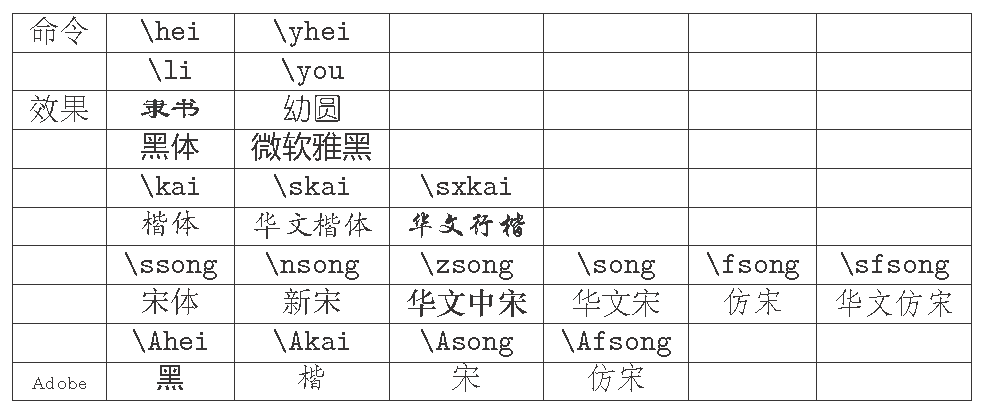
\includegraphics{figs/winfonts.png}
% \end{figure}
% \subsection{学校配色与Logo}
% \subsubsection{配色}
% 学校的配色示例文件在 \pkg{beamercolorthemeustc.sty}, 自己可以仿照配置模板
% 颜色.
% \subsubsection{Logo}
%   你可以使用 \opt{logo} 选项来在报告首页生成学校和学院的logo. 
%   学校与学院的Logo都放在 \file{logo/} 目录下. 
%   这个对不同学校而言当然是不同
%   的, 如果你要使用自己学校的logo, 请注意以下
%   \begin{itemize}
%     \item 两个logo的高度都为 \opt{1cm}, 而且都没有背景
%	格式为pdf. 请使用图像处理软件(GIMP)处理;
%     \item 图标的颜色应该和整个模板的配色协调. 故你要么更改图标的颜色,%       要么更改本模板的配色;
%     \item 最后你还需要检查背景色和前景色的配合是否具有高对比度(字体能
%	看清), 我使用的是\href{http://contrastchecker.com/}
%	{Contrast Checker}.
%   \end{itemize}
% \subsection{定理环境的使用}
% \subsubsection{自带定理环境}
% \pkg{beamer} 自身已经定义了定理环境\cite{tantau2004user}*{p.~193}: 
% \env{theorem}, \env{lemma}, \env{definition},
% \env{corollary}, \env{example}, 
% \env{proposition}(好像我不能使用 \env{proposition})
% \begin{latex}
%   \begin{theorem}[勾股定理]
%     假设$a,b,c$是直角三角形的三边, 且$c>a\geq b>0$, 则
%     \[
%	a^a+b^2=c^2.
%     \]
%   \end{theorem}
% \end{latex}
% \subsubsection{预定义定理环境}
% 除了beamer默认定义的定理环境, 本模板还自带定义了一些定理环境,
% 具体请参考配置文件: \file{ustcmb.cfg}.
%
% 这里举例如下
% \begin{latex}
%  \begin{thm}[勾股定理]
%     假设$a,b,c$是直角三角形的三边, 且$c>a\geq b>0$, 则
%     \[
%	a^a+b^2=c^2.
%     \]
%   \end{thm}
% \end{latex}
% \subsubsection{定理环境的变式}
% 定理环境有两个变式, 即 \env{Block} 与 \env{AlertBlock}. 示例如下:
% \begin{latex}
%   \begin{block}{Block Title}
%     Block示例
%   \end{block}
%   \begin{alertblock}
%     AlertBlock示例
%   \end{alertblock}
% \end{latex}
% \subsubsection{长定理的写法}
% 在实际写作中, 我们可能遇到一个定理太长, 需要分两个 \env{frame} 来写.
% 此时可以使用如下的例子来手动分页:
% \begin{latex}
%   \begin{thm}
%     长定理的内容, 超过一页
%   \end{thm}
%   \adtocounter{thm}{-1}
%   \begin{thm}[Cont.]
%     长定理超过一页的部分
%   \end{thm}
% \end{latex}
% 这里的要点是通过重置 \env{thm} 的编号来实现定理编号的正确.
% \subsection{自动分页与\env{itemize}的分步显示}
% 我们知道, 可以对\env{frame}使用选项\opt{allowframebreaks}来自动分页。
% 但是这种方法会使得分步显示无效。解决办法是使用cover:
% \begin{latex}
%   \begin{frame}[<+->]{自动分页与分步显示}
%     \begin{onlyenv}<1>
%       第一页内容
%     \end{onlyenv}
%     \begin{onlyenv}<2->
%       第二页放置一个列表
%       \begin{itemize}[<+(1)->]
%         \item 第一项
%         \item 第二项
%       \end{itemize}
%       我们应该注意到\opt{(+1)}, 它表示将暂停计数器(beamerpause)
%       加1, 从而第一项在第二帧显示, 而第二项在第3帧显示.
%     \end{onlyenv}
%   \end{frame} 
% \end{latex}
% \subsection{打印模式}
% 本模板提供了方便打印slide的模式 \opt{print}, 使用该模式会作如下改变
% \begin{itemize}
%   \item 主题颜色设置灰色, 并且带有灰度背景, 方便查看是否超出边距;
%   \item 4张幻灯片放到一页A4(横向)纸上;
%   \item 同一个frame中的多个遮罩(overlay)会合并到一页打印;
%   \item 由于默认使用的是 \opt{handout} 模式来打印, 参考文献列表不会打印.
% \end{itemize}
% \subsection{反馈}
% 非常感谢你使用本模板, 若你在使用过程中有任何疑问/建议. 
% 请不要吝啬, 将其反馈到模板
% \href{https://github.com/vanabel/mathbeamer/issues}{发布主页}.
%
% 此外你还可以加入QQ群\href{https://goo.gl/i1kcwe}{LaTeX讨论区}.
% \StopEventually{}
% \section{类文件源码}
%    \begin{macrocode}
%<*class>
%    \end{macrocode}
% \subsection{宏包依赖}
% 使用 \pkg{etoolbox} 来设置启用/禁用选项
%    \begin{macrocode}
\RequirePackage{etoolbox}
\RequirePackage{xcolor}
%    \end{macrocode}
% 数学定理与字体支持
%    \begin{macrocode}
\RequirePackage{mathtools, bm}
%    \end{macrocode}
% 英文断行
%    \begin{macrocode}
\RequirePackage[english]{babel}
%    \end{macrocode}
% 超链接
%    \begin{macrocode}
\AtBeginDocument{
  \RequirePackage{hyperref}
  \hypersetup{
    pdfpagemode=FullScreen,
    bookmarksopen=false,
    pdfencoding=auto,
    colorlinks=true,
    %ocgcolorlinks,
    %pdfusetitle
  }
}
%    \end{macrocode}
% \subsection{选项申明}
% \opt{print}选项: 编译打印版本
%    \begin{macrocode}
\providetoggle{print}
\DeclareOption{print}{\toggletrue{print}}
%    \end{macrocode}
% \opt{nds}选项: 不启用默认设置
%    \begin{macrocode}
\newif\ifMB@nds\MB@ndsfalse
\DeclareOption{nds}{\MB@ndstrue}
%    \end{macrocode}
% \opt{thmnum}选项: 定理有编号
%    \begin{macrocode}
\newif\ifMB@thmnum\MB@thmnumfalse
\DeclareOption{thmnum}{\MB@thmnumtrue}
%    \end{macrocode}
% \opt{subnav}选项:插入小节导航
%    \begin{macrocode}
\newif\ifMB@subnav\MB@subnavfalse
\DeclareOption{subnav}{\MB@subnavtrue}
%    \end{macrocode}
% \opt{eqsecnum}选项: 以节编号公式
%    \begin{macrocode}
\newif\ifMB@eqsecnum\MB@eqsecnumfalse
\DeclareOption{eqsecnum}{\MB@eqsecnumtrue}
%    \end{macrocode}
% \opt{authoryear}选项: 作者年代(bibtex)引用方式
%    \begin{macrocode}
\newif\ifMB@authoryear\MB@authoryearfalse
\DeclareOption{authoryear}{\MB@authoryeartrue}
%    \end{macrocode}
% \opt{allcite}选项: 列出所有参考文献
%    \begin{macrocode}
\newif\ifMB@allcites\MB@allcitesfalse
\DeclareOption{allcites}{\MB@allcitestrue}
%    \end{macrocode}
% \opt{nobib}选项: 去掉参考文献列表
%    \begin{macrocode}
\newif\ifMB@nobib\MB@nobibfalse
\DeclareOption{nobib}{\MB@nobibtrue}
%    \end{macrocode}
% \opt{biblatex}选项: 使用现代biblatex包替代amsrefs
%    \begin{macrocode}
\newif\ifMB@biblatex\MB@biblatexfalse
\DeclareOption{biblatex}{\MB@biblatextrue}
%    \end{macrocode}





% \opt{citemath}选项: biblatex的数学论文专用引用样式(需要xstring包)
%    \begin{macrocode}
\newif\ifMB@citemath\MB@citemathfalse
\DeclareOption{citemath}{\MB@citemathtrue}
%    \end{macrocode}

% \opt{zh}选项: 中文模式
%    \begin{macrocode}
\DeclareOption{zh}{\MB@zhtrue}
\newif\ifMB@zh\MB@zhfalse
%    \end{macrocode}
% \opt{logo}选项: 使用logo
%    \begin{macrocode}
\DeclareOption{logo}{\MB@logotrue}
\newif\ifMB@logo\MB@logofalse
%    \end{macrocode}
% 传递参数
%    \begin{macrocode}
\DeclareOption*{\PassOptionsToClass{\CurrentOption}{beamer}}
\ProcessOptions\relax
%    \end{macrocode}
% 提供标准的类声明
%    \begin{macrocode}
\ProvidesClass{ustcmb}[2025/08/21 v2.2.5 USTC Math Beamer Template]
%    \end{macrocode}
% \subsection{基于模式加载文档类}
% 如果是打印(\opt{print})模式
%    \begin{macrocode}
\iftoggle{print}{
  \LoadClass[handout, nds]{beamer}
  \RequirePackage{pgfpages}
  \pgfpagesuselayout{4 on 1}[a4paper,border shrink=5mm,landscape]
  \mode<handout>{\setbeamercolor{background canvas}{bg=black!5}}
}
%    \end{macrocode}
% 否则是报告模式, 生成报告
%    \begin{macrocode}
{
  \LoadClass{beamer}
}
%    \end{macrocode}
% \subsection{选项实现}
% \opt{zh}选项: 表示使用中文模式
%    \begin{macrocode}
\ifMB@zh
%    \end{macrocode}
% ctex 中文支持引擎
%    \begin{macrocode}
\RequirePackage{ctex}
%    \end{macrocode}
%% 中文模式下字体配置, 主要更改了标题(title)/帧标题(frametitle)/正文(normal text). 其他结构的修改可以参考\href{http://www.cpt.univ-mrs.fr/~masson/latex/Beamer-appearance-cheat-sheet.pdf}{Beamer appearance cheat sheet}.
%    \begin{macrocode}
\ifMB@zh
\setbeamerfont*{title}{family=\sffamily, shape=\scshape, series=\bfseries, size=\LARGE}
\setbeamerfont{frametitle}{family=\sffamily, shape=\upshape, series=\bfseries}
\setbeamerfont{normal text}{family=\rmfamily, shape=\upshape, series=\mdseries}
\AtBeginDocument{\usebeamerfont{normal text}}
\fi
%    \end{macrocode}
%% 中文强调
%    \begin{macrocode}
\RequirePackage{ulem}
\AtEndOfClass{% ^^A documentation part start with %
% ^^A All other parts are called definition parts
% ^^A Comments in documentation part
% ^^A equivalently use \iffalse ... \fi
% \iffalse meta-comment
% !TeX program = XeLaTeX
% !TeX encoding = UTF-8

% This work may be distributed and/or modified under the
% conditions of the LaTeX Project Public License, either
% version 1.3c of this license or (at your option) any later
% version. This version of this license is in
%    http://www.latex-project.org/lppl/lppl-1-3c.txt
% and the latest version of this license is in
%    http://www.latex-project.org/lppl.txt
% and version 1.3 or later is part of all distributions of
% LaTeX version 2005/12/01 or later.
%
% This work has the LPPL maintenance status `maintained'.
%
% The Current Maintainers of this work is Van Abel.
%
% ---------------------------------------------------------------------
%
%<*internal>
\iffalse
%</internal>
%<*readme>
# ustcmb --- 数学类报告模板

[![License](https://img.shields.io/badge/License-LPPL%20v1.3c-blue.svg)](http://www.latex-project.org/lppl.txt)
[![Version](https://img.shields.io/badge/Version-v2.2.4-green.svg)](https://github.com/vanabel/mathbeamer)
[![LaTeX](https://img.shields.io/badge/LaTeX-Beamer-orange.svg)](https://www.ctan.org/pkg/beamer)

> 基于USTC学校主题定制的数学报告模板,支持中英文双语,提供良好的打印模式

## 📖 简介

`ustcmb` (ustcmethbeamer) 是基于USTC学校主题定制的报告模板,利用它可以非常方便地制作数学类幻灯片。它同时支持中文与英文的处理,以及良好的打印模式。

### ✨ 主要特性

- 🎨 基于USTC学校主题的现代化设计
- 🌏 完整的中英文双语支持
- 📚 灵活的参考文献处理(支持amsrefs和biblatex)
- 🎯 丰富的定理环境配置选项
- 🖨️ 优化的打印模式支持
- 📱 响应式布局设计

## 🚀 快速开始

### 下载安装

1. 下载模板压缩包:[最新版本](https://github.com/vanabel/mathbeamer/releases/latest)
2. 解压后阅读示例文件 `ustcmb-main.pdf`
3. 参考 `ustcmb-main.tex` 开始编写您的报告

### 基本使用

```latex
\documentclass[zh]{ustcmb}

\title{您的报告标题}
\author{您的姓名}
\institute{您的机构}

\begin{document}
\frame{\titlepage}

\begin{frame}
\frametitle{第一张幻灯片}
内容...
\end{frame}

\end{document}
```

## ⚙️ 配置选项

### 核心选项

| 选项 | 描述 | 默认值 |
|------|------|--------|
| `zh` | 启用中文支持 | 启用 |
| `en` | 英文模式 | 禁用 |
| `thmnum` | 定理带编号 | 禁用 |
| `eqsecnum` | 公式以节编号 | 禁用 |

### 参考文献选项

| 选项 | 描述 | 依赖 |
|------|------|------|
| `authoryear` | 作者年代引用样式 (amsrefs) | amsrefs |
| `allcites` | 输出bib.bib中的所有参考文献 | amsrefs |
| `biblatex` | 使用现代biblatex包 | biblatex |
| `citemath` | 数学论文专用引用样式 | biblatex + xstring |

### 高级选项

| 选项 | 描述 |
|------|------|
| `nds` | 不使用默认设置(需要手动配置) |
| `subnav` | 在每个子节显示导航 |
| `nobib` | 禁用参考文献处理 |

## 📚 示例文件

项目包含多个示例文件,帮助您快速上手:

- `ustcmb-main.tex` - 主要示例文件
- `biblatex-example.tex` - biblatex使用示例
- `amsrefs-example.tex` - amsrefs使用示例
- `math-citation-example.tex` - 数学引用示例

## 🔧 自定义配置

### 使用nds选项时的必要配置

当使用 `nds` 选项时,您需要手动配置以下内容:

```latex
\documentclass[nds]{ustcmb}

% 设置主题
\usetheme{YourTheme}

% 设置标题页
\begin{document}
\frame{\titlepage}

% 设置定理环境
\newtheorem{thm}{Theorem}

% 可选:设置颜色主题
\usecolortheme{YourColorTheme}
```

### 字体配置

模板支持自定义中文字体:

```latex
% 在导言区设置
\setCJKmainfont{YourChineseFont}
\setCJKsansfont{YourChineseSansFont}
```

## 📋 版本历史

### [v2.2.4] (开发中)

- ✨ 新增 `biblatex` 选项,支持现代参考文献处理
- ✨ 新增多种引用样式选项
- 🔄 保持对传统 `amsrefs` 的向后兼容性
- ⚡ 优化参考文献配置和引用格式

### [v2.2.3]

- ✨ 新增 `nobib` 选项
- 🧹 移除多余的参考文献导航
- 🔤 重新设置中文字体,支持Mac和Windows系统
- 🎨 重新配置模板标题/正文字体

### [v2.2.2]

- ✨ 新增中文自定义字体命令

### [v2.2.1]

- 🐛 修复 `\CJKunderwave` 兼容性问题

### [v2.2.0]

- ✨ 新增 `subnav` 选项:在每个子节显示导航
- 📖 添加解决 `allowframebreaks` 和 `itemize` 环境冲突的示例
- 🗑️ 移除"Thanks!"页面,应由演示总结替代

### [v2.1.0]

- 🏫 新增SJTU标志支持
- ✨ 为SJTU添加 `domc` 选项

### [v2.0.1]

- 📚 新增用户FAQ
- 🌏 根据 `zh` 或 `en` 模式修改最后一帧的感谢内容

### [v2.0.0]

- 🔧 使用dtx管理文档
- 🗑️ 移除xeCJK字体设置(应由用户自行配置)

### [v1.2.0]

- 🌏 新增中文支持选项,使用 `zh` 启用中文支持
- 🎨 新增默认颜色主题,更接近USTC颜色(主色调为蓝色)

### [v 1.1.1]

1. add more example slides, which includes
 * auto pause in lists
 * two columns in a frame
 * include figure/subfigures in a frame
 * table
 * definition/example/theorem like environments
 * custom defn/examp/thm theorem like environments
 * hyperlinks between slides
2. add thanks before the references
3. user defined commands/environments should be written in `slides/usrdefn.tex`

#### [v 1.1.0]

1. new branch, add three color style:
 * `dark`: dark color style
 * `light`: light color style
 * the default is betwen the above two

#### [v 1.0.1]

1. add link to `slides/bib.bib`, so that you can open it in `WinEdt` by `Build Tree`
2. set the default font theme for math be `\usefonttheme{professionalfonts}`, which makes math formula looks more perfect
3. add `\newcommand{}{}` example and `\newtheorem{}{}` example

### Copyright and Licence

Copyright (C) 2016 by Van Abel <van141.abel@gmail.com>

This work may be distributed and/or modified under the
conditions of the LaTeX Project Public License, either version 1.3
of this license or (at your option) any later version.
The latest version of this license is in

http://www.latex-project.org/lppl.txt

and version 1.3 or later is part of all distributions of LaTeX
version 2005/12/01 or later.

    This work consists of the file: ustcmb.dtx 
             and the derived files: ustcmb.ins
                                    ustcmb.cls
                                    ustcmb.tex
                                    ustcmb.cfg
                                    beamercolorthemeustc.sty
                                    READEME.md (this file)
%</readme>
%<*internal>
\fi    
\def\nameoflatex{plain}
\ifx\nameoflatex\fmtname\else
  \expandafter\begingroup
\fi
%</internal>
%
%<*install>

\input docstrip.tex
\keepsilent

\preamble
----------------------------------------------------------------
    模板名称: ustcmb 
        描述: 中科大数学报告模板
    模板网址: https://github.com/vanabel/mathbeamer
      版本号: v2.2.3
        作者: Van Abel
      E-mail: van141.abel@gmail.com
     License: LaTeX Project Public License v1.3c or later
 License URI: http://www.latex-project.org/lppl.txt
----------------------------------------------------------------

\endpreamble
\postamble

This is a generated file

Copyright (C) 2016 by Van Abel <van141.abel@gmail.com>

This work may be distributed and/or modified under the
conditions of the LaTeX Project Public License, either version 1.3
of this license or (at your option) any later version.
The latest version of this license is in

http://www.latex-project.org/lppl.txt

and version 1.3 or later is part of all distributions of LaTeX
version 2005/12/01 or later.

This work consists of the file ustcmb.dtx
and the derived files:
  ustcmb.ins
  ustcmb.cls
  ustcmb.tex
  ustcmb.cfg
  beamercolorthemeustc.sty

\endpostamble
\askforoverwritefalse
\generate{
  \usedir{tex/latex/ustcmb}
  \file{\jobname.cls}{\from{\jobname.dtx}{class}}
  \file{\jobname.cfg}{\from{\jobname.dtx}{cfg}}
  \file{beamercolorthemeustc.sty}{\from{\jobname.dtx}{ustc}}
  \nopreamble\nopostamble
  \usedir{doc/latex/ustcmb}
  \file{\jobname-main.tex}{\from{\jobname.dtx}{main}}
}
\obeyspaces
\Msg{****************************************************}
\Msg{*                                                   }
\Msg{* To finish the installation you have to move the   }
\Msg{* following file into a directory searched by TeX   }
\Msg{* e.g. tex/latex/ustcmb:                            }
\Msg{*                                                   }
\Msg{* \jobname.cls                                      }
\Msg{* \jobname.cfg                                      }
\Msg{* beamercolorthemeustc.sty                          }
\Msg{*                                                   }
\Msg{* To produce the documentation run the file         }
\Msg{* \jobname.dtx through XeLaTeX.                     }
\Msg{*                                                   }
\Msg{* To produce the sample file run the file           }
\Msg{* \jobname-main.tex through XeLaTeX and BibTeX      }
\Msg{*                                                   }
\Msg{* Happy TeXing!                                     }
\Msg{*                                                   }
\Msg{****************************************************}
%</install>
%<install>\endbatchfile
%
%<*internal>
\usedir{source/latex/ustcmb}
\generate{
  \file{\jobname.ins}{\from{\jobname.dtx}{install}}
}
% ^^A No extra text add by DocStrip
\nopreamble\nopostamble
\usedir{doc/latex/ustcmb}
\generate{
  \file{README.md}{\from{\jobname.dtx}{readme}}
}
% ^^A if xetex then end process of DocStrip by \endbatchfile
\ifx\nameoflatex\fmtname
  \expandafter\endbatchfile
\else
% ^^A for xelatex we close the group
  \expandafter\endgroup
\fi
%</internal>
%
%<*driver>
\ProvidesFile{\jobname.dtx}
%</driver>
%<class>\NeedsTeXFormat{LaTeX2e}[2005/12/01]
%<class>\ProvidesClass{ustcmb}
%<*class>
[2025/08/21 v2.2.4 中科大数学报告模板类文件]
%</class>
%
%<*driver>
\documentclass{ltxdoc}
\usepackage{xeCJK}
\setCJKmainfont[AutoFakeBold, ItalicFont=STKaiti]{STSong}
\setCJKsansfont[AutoFakeBold, AutoFakeSlant]{STXihei}
\setCJKmonofont[AutoFakeBold, AutoFakeSlant]{STFangsong}
\setlength\parindent{0pt}
\usepackage{booktabs,tabularx}
\usepackage{metalogo}
\usepackage{hypdoc}
\hypersetup{
  bookmarksopen=true,
  bookmarksopenlevel=2,
  bookmarksnumbered=true,
  CJKbookmarks=true,
  unicode=true,
  allcolors=blue,
}
\usepackage{xcolor} % use lightgray
\usepackage[alphabetic, msc-links, lite, abbrev]{amsrefs}
\usepackage{listings}
\lstdefinestyle{lstshell}{
  basicstyle=\small\ttfamily,
  backgroundcolor=\color{red!75!black},
  gobble=2,% 重要!否则会生成注释符号"%"
language=bash}
\lstdefinestyle{lstlatex}{
  basicstyle=\small\ttfamily,
  frame=single,
  gobble=2,
language=[LaTeX]TeX}
\lstnewenvironment{shell}{\lstset{style=lstshell}}{}
\lstnewenvironment{latex}{\lstset{style=lstlatex}}{}
\newcommand\shellcmd[1]{ \underline{\texttt{#1}}}
\EnableCrossrefs
\CodelineIndex
%\OnlyDescription
% 模仿 l3doc 的定义
\DeclareRobustCommand\file{\nolinkurl}
\DeclareRobustCommand\env{\texttt}
\DeclareRobustCommand\pkg{\textsf}
\DeclareRobustCommand\cls{\textsf}
\DeclareRobustCommand\opt{\textbf}

\renewcommand\indexname{命令索引}
\IndexPrologue{%
  \section*{\indexname}
  \textit{斜体的数字表示描述对应索引项的页码;
    带下划线的数字表示定义对应索引项的代码行号;
  罗马字体的数字表示使用对应索引项的代码行号。}
}
\RecordChanges
\def\glossaryname{版本历史}
\GlossaryPrologue{\section*{\glossaryname}}

\begin{document}
\DocInput{\jobname.dtx}
\renewcommand{\refname}{参考文献}
\begin{thebibliography}{9}
\bibitem{tantau2004user} 
Tantau, Till.
\textit{User's Guide to the Beamer Class, Version 3.01}. 
2004
\bibitem{xecjk2016manual}
CTEX.ORG.
\textit{xeCJK宏包手册}.
2006
\end{thebibliography}
\PrintChanges
\PrintIndex
\end{document}
%</driver>
% \fi
%
%
% \CharacterTable
%  {Upper-case    \A\B\C\D\E\F\G\H\I\J\K\L\M\N\O\P\Q\R\S\T\U\V\W\X\Y\Z
%   Lower-case    \a\b\c\d\e\f\g\h\i\j\k\l\m\n\o\p\q\r\s\t\u\v\w\x\y\z
%   Digits        \0\1\2\3\4\5\6\7\8\9
%   Exclamation   \!     Double quote  \"     Hash (number) \#
%   Dollar        \$     Percent       \%     Ampersand     \&
%   Acute accent  \'     Left paren    \(     Right paren   \)
%   Asterisk      \*     Plus          \+     Comma         \,
%   Minus         \-     Point         \.     Solidus       \/
%   Colon         \:     Semicolon     \;     Less than     \<
%   Equals        \=     Greater than  \>     Question mark \?
%   Commercial at \@     Left bracket  \[     Backslash     \\
%   Right bracket \]     Circumflex    \^     Underscore    \_
%   Grave accent  \`     Left brace    \{     Vertical bar  \|
%   Right brace   \}     Tilde         \~}
% \changes{v2.2.4}{2025/08/21}{新增\opt{biblatex}选项,支持现代参考文献处理}
% \changes{v2.2.4}{2025/08/21}{新增\opt{citemath}选项,支持数学论文专用引用样式}
% \changes{v2.2.4}{2025/08/21}{保持对传统\pkg{amsrefs}的向后兼容性}
% \changes{v2.2.4}{2025/08/21}{优化参考文献配置和引用格式}
% \changes{v2.2.3}{2018/06/03}{移除多余的参考文献导航}
% \changes{v2.2.3}{2018/06/03}{重新设置中文字体,使得Mac系统和Windows系统都可用}
% \changes{v2.2.3}{2018/06/03}{新增\shellcmd{nobib}选项}
% \changes{v2.2.2}{2018/06/02}{新增中文字体命令}
% \changes{v2.2.1}{2018/04/05}{修复\env{CJKunderwave}的不兼容性}
% \changes{v2.2.0}{2017/11/29}{新增小节导航选项\opt{subnav}}
% \changes{v2.2.0}{2017/11/29}{新增示例:\opt{allowframebreaks}与\env{itemize}分步显示}
% \changes{v2.2.0}{2017/11/29}{移出致谢页,因为在报告结束应该呈现一个你报告主题的摘要而非简单的``谢谢''两个字}
% \changes{v2.1.0}{2017/11/07}{新增上海交大学院与学校logo}
% \changes{v2.1.0}{2017/11/07}{新增用户快速配色, 只需改变主配色\shellcmd{domc}的值, 详见示例文档\file{math-beamer.tex}}
% \changes{v2.0.1}{2017/04/30}{提供用户使用FAQ}
% \changes{v2.0.1}{2017/04/30}{修改致谢/Thanks以匹配语言}
% \changes{v2.0.0}{2016/12/14}{使用dtx管理文档}
% \changes{v1.2.0}{2016/05/15}{Add chinese support option, just use `zh` to support chinese}
% \changes{v1.2.0}{2016/05/15}{Add default colortheme to be more like USTC color (blue in main)}
% \changes{v1.1.1}{2015/09/21}{Add more example slides}
% \changes{v1.1.1}{2015/09/21}{Add thanks before the references}
% \changes{v1.1.1}{2015/09/21}{Add user-defined commands/environments in \file{slides/usrdefn.tex}}
% \changes{v1.1.0}{2015/09/20}{New branch, add three color style}
% \changes{v1.0.1}{2015/09/20}{Add links supported by WinEdt Build Tree to \file{slides/bib.bib}}
% \changes{v1.0.1}{2015/09/20}{Add |newcommand| and |newtheorem| examples}
% \changes{v1.0.0}{2015/09/19}{Initial version}

% \GetFileInfo{\jobname.dtx}
%
% \DoNotIndex{\%,\#,\$,\%,\&,\@,\\,\{,\},\^,\_,\~,\ ,\[,\],\documentclass}
% \DoNotIndex{\@ne,\and,\author,\centerline,\date,\inst,\institute}
% \DoNotIndex{\definecolor,\decumentclass,\label,\newtheorem,\sc}
% \DoNotIndex{\setbeamercolor,\setbeamercovered,\setbeamertemplate}
% \DoNotIndex{\cite,\uwave,\cline,\eps,\epsilon,\geq}
% \DoNotIndex{\hline,\href,\item,\jobname,\lipsum,\lstinline}
% \DoNotIndex{\lstset,\small,\subsection,\textwidth,\ttfamily}
% \DoNotIndex{\tableofcontents, \setCJKmainfont,\setbeamerfont}
% \DoNotIndex{\setCJKmonofont,\setCJKsansfont,\subject,\subtitle}
% \DoNotIndex{\theoremstyle, \title, \titlepage, \usepackage}
% \DoNotIndex{\advance,\begingroup,\catcode,\closein}
% \DoNotIndex{\closeout,\day,\def,\edef,\else,\empty,\endgroup}
% \DoNotIndex{\addtobeamertemplate, \addtocounter}
% \DoNotIndex{\AtBeginDocument,\AtEndDocument,\AtEndOfClass}
% \DoNotIndex{\begin,\end,\bfseries,\bibliography}
% \DoNotIndex{\color,\CurrentOption,\DeclareOption,\fi,\frame}
% \DoNotIndex{\hfill,\hypersetup,\iftoggle,\includegraphics,\input}
% \DoNotIndex{\insertframenumber,\inserttotalframenumber}
% \DoNotIndex{\mode,\LARGE,\LoadClass,\necounter,\noewif,\nocite}
% \DoNotIndex{\numberwithin,\PassOptionsToClass,\pgfpagesuselayout}
% \DoNotIndex{\ProcessOptions, \providetoggle,\relax,\renewcommand}
% \DoNotIndex{\RequirePackage, \section, \setcounter, \toggletrue}
% \DoNotIndex{\value,\newcommand,\newif,\newcounter}
% \DoNotIndex{\ccwd,\caption,\captionsetup,\chapter,\ctexset}
% \DoNotIndex{\itemsep,\hangindent,\setfontsize,\setlength,\hdclindex}
% \DoNotIndex{\textbf,\newenvironment,\newcommand}
% \DoNotIndex{\n,\newCJKfontfamily,\AtBeginSubsection}
% \expandafter\DoNotIndex\expandafter{\string\&}
%
% \title{\textsf{ustcmb}类用户手册\thanks{这是
%   \textsf{ustcmb}~\fileversion 的用户使用说明文档,
%   创建于 \filedate.}}
% \author{Van Abel \\ \texttt{\small van141.abel@gmail.com}}
% \date{\filedate}
%
% \maketitle
% \def\abstractname{摘要}
% \begin{abstract}
%   \cls{ustcmb}是我准备博士论文答辩时制作的模板. 它主要是为了方便数学
%   专业的同学写报告. 其中定义了几个选项方便快速实现功能定制, 而且还配
%   置了与USTC学校主页相适配的主题以及显示学校/学院Logo.
%
%   \cls{ustcmb.cls}文档类只支持\XeLaTeX{}方式编译. 模板提供了示例文件 \file{\jobname-main.tex}以及配色文件 \pkg{beamercolorthemeustc.sty}.
% \end{abstract}
% 
% \section{简介}
% 
%   本报告模板旨在方便大家轻松上手制作报告. 在一定程度上定制报告格式,
%   应大家要求还同时支持中文和英文. 支持选项如下:
% \begin{table}[htbp]
%   \begin{tabular}{|l|p{.75\textwidth}|}
%     \hline
%     \opt{zh} & 中文支持(ctex) \\
%     \hline
%     \opt{logo} & 使用学校以及学院Logo \\
%     \hline
%     \opt{thmnum} & 定理编号\\
%     \hline
%     \opt{eqsecnum} & 公式以节编号\\
%     \hline
%     \opt{subnav} & 在每小节开始显示小节导航\\
%     \hline
%     \opt{authoryear} & 作者年代型文献引用(amsrefs)\\
%     \hline
%     \opt{allcites} & 自动列出所有参考文献\\
%     \hline
%     \opt{biblatex} & 使用现代biblatex包替代amsrefs\\
%     \hline

%     \hline


%     \opt{citemath} & biblatex数学论文专用引用样式(需要xstring包)\\
%     \hline
%     \opt{nds} & 不使用默认设置\\
%     \hline
%     \opt{nobib} & 不列出参考文献\\
%     \hline
%     \opt{print} & 打印模式\\
%     \hline
%   \end{tabular}
% \end{table}
% \section{模板生成与安装} 
% 本发行版已经包含所有的生成文件. 所以, 如果您对如何生成模板文件
% 不感兴趣, 则完全可以跳过这一节.
% 
% 模板解压缩后生成文件夹 \file{ustcmb-vN.M}, 其中 \file{vN.M} 为版本号. 
% 该文件夹包含以下文件
% \begin{itemize}
%  \item \file{ustcmb.dtx}: 模板文档源文件
%  \item \file{ustcmb.tex}: 模板示例文件
%  \item \cls{ustcmb.cls}: 模板类文件
%  \item \file{ustcmb.cfg}: 英文/中文定理配置文件
%  \item \pkg{beamercolorthemeustc.sty}: 模板配色文件
% \end{itemize}
% Linux/Mac用户可以直接使用 GNU make 工具, 
% Windows用户建议安装 \href{https://www.cygwin.com/}{Cygwin}
% 然后同样使用 GUN make 工具.
% \begin{itemize}
%  \item 编译文档\shellcmd{make doc}
%  \item 编译示例文件\shellcmd{make main}
%  \item 安装模板到TeX系统\shellcmd{make inst}
%  \item 以管理员方式安装模板到TeX系统\shellcmd{make install}
%  \item 从TeX系统卸载模板\shellcmd{make uninst}
%  \item 以管理员方式从TeX系统卸载模板\shellcmd{make uninstall}
%  \item 清空临时文件\shellcmd{make clean}
%  \item 清空所有生成文件\shellcmd{make distclean}
%  \item 打包文件以发布\shellcmd{make zip}
% \end{itemize}
% \section{使用手册}
% 这节主要讲一讲支持的选项. 
% \subsection{中文支持}
% 中文采用的是 \pkg{ctex} 方案, 使用时只需添加 \opt{zh} 选项即可.
% 
% 需要注意的是, 默认状态下\texttt{并没有配置任何中文字体}. 
% 故可能产生以下问题:
% \begin{itemize}
%   \item 在旧版本的\pkg{xeCJK} 中编译不通过(因为没有默认配置字体). 
%     此时需要升级 \pkg{xeCJK} 包即可.
%   \item \pkg{xeCJK} 默认的字体是黑体, 也许不适用于正式场合. 
%   \item 如何查看以及使用字体, 请参考\cite[p.~8, 3.2.1节]
%     {xecjk2016manual}. 例如你可以在导言区加入
%   \begin{latex}	    
%     \setCJKmainfont[AutoFakeSlant, AutoFakeBold]{SimSun}
%     \setCJKmonofont[AutoFakeSlant, AutoFakeBold]{FangSong}
%     \setCJKsansfont[AutoFakeSlant, AutoFakeBold]{KaiTi}
%   \end{latex}
%   如果你要使用黑体为正文字体,只需将上述命令修改为
%   \begin{latex}
%     \setCJKmainfont[AutoFakeSlant, AutoFakeBold]{SimHei}
%   \end{latex}
% \end{itemize}
% 此外,在v2.2.2版中,还增加了一些默认的字体命令,但是这些字体默认都没有启用,要使用这些字体命令,
% 请进行如下操作:
% \begin{enumerate}
%   \item 打开根目录下的\file{ustcmb.cfg}, 去掉你想要使用的字体前的两个百分号,例如
%     \begin{latex}
% %%  微软雅黑
% %%  \newCJKfontfamily[yhei]\yhei{Microsoft YaHei}
%     \end{latex}
%   \item 在\file{ustcmb-main.tex}的正文中使用(当然你得确保系统由微软雅黑字体)
%     \begin{latex}
% 正文{\yhei 这是雅黑}正文
%     \end{latex}
% \end{enumerate}
% \begin{figure}[htbp]
%   \centering
%   \caption{完整的字体列表与效果}
%   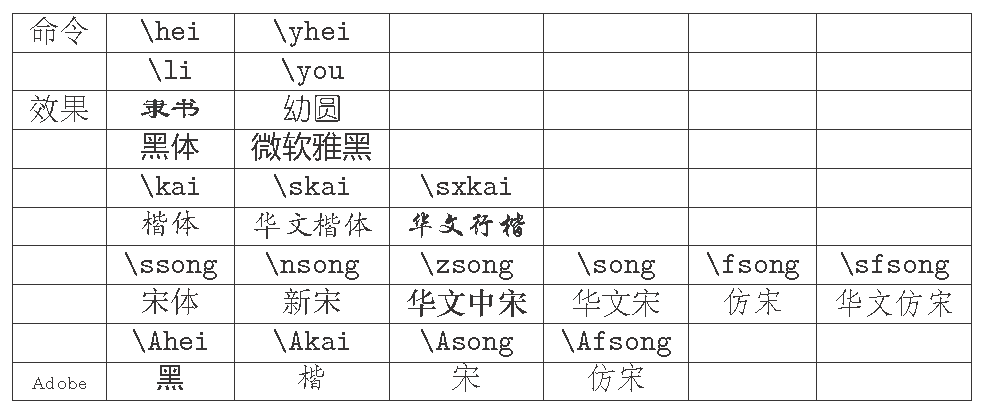
\includegraphics{figs/winfonts.png}
% \end{figure}
% \subsection{学校配色与Logo}
% \subsubsection{配色}
% 学校的配色示例文件在 \pkg{beamercolorthemeustc.sty}, 自己可以仿照配置模板
% 颜色.
% \subsubsection{Logo}
%   你可以使用 \opt{logo} 选项来在报告首页生成学校和学院的logo. 
%   学校与学院的Logo都放在 \file{logo/} 目录下. 
%   这个对不同学校而言当然是不同
%   的, 如果你要使用自己学校的logo, 请注意以下
%   \begin{itemize}
%     \item 两个logo的高度都为 \opt{1cm}, 而且都没有背景
%	格式为pdf. 请使用图像处理软件(GIMP)处理;
%     \item 图标的颜色应该和整个模板的配色协调. 故你要么更改图标的颜色,%       要么更改本模板的配色;
%     \item 最后你还需要检查背景色和前景色的配合是否具有高对比度(字体能
%	看清), 我使用的是\href{http://contrastchecker.com/}
%	{Contrast Checker}.
%   \end{itemize}
% \subsection{定理环境的使用}
% \subsubsection{自带定理环境}
% \pkg{beamer} 自身已经定义了定理环境\cite{tantau2004user}*{p.~193}: 
% \env{theorem}, \env{lemma}, \env{definition},
% \env{corollary}, \env{example}, 
% \env{proposition}(好像我不能使用 \env{proposition})
% \begin{latex}
%   \begin{theorem}[勾股定理]
%     假设$a,b,c$是直角三角形的三边, 且$c>a\geq b>0$, 则
%     \[
%	a^a+b^2=c^2.
%     \]
%   \end{theorem}
% \end{latex}
% \subsubsection{预定义定理环境}
% 除了beamer默认定义的定理环境, 本模板还自带定义了一些定理环境,
% 具体请参考配置文件: \file{ustcmb.cfg}.
%
% 这里举例如下
% \begin{latex}
%  \begin{thm}[勾股定理]
%     假设$a,b,c$是直角三角形的三边, 且$c>a\geq b>0$, 则
%     \[
%	a^a+b^2=c^2.
%     \]
%   \end{thm}
% \end{latex}
% \subsubsection{定理环境的变式}
% 定理环境有两个变式, 即 \env{Block} 与 \env{AlertBlock}. 示例如下:
% \begin{latex}
%   \begin{block}{Block Title}
%     Block示例
%   \end{block}
%   \begin{alertblock}
%     AlertBlock示例
%   \end{alertblock}
% \end{latex}
% \subsubsection{长定理的写法}
% 在实际写作中, 我们可能遇到一个定理太长, 需要分两个 \env{frame} 来写.
% 此时可以使用如下的例子来手动分页:
% \begin{latex}
%   \begin{thm}
%     长定理的内容, 超过一页
%   \end{thm}
%   \adtocounter{thm}{-1}
%   \begin{thm}[Cont.]
%     长定理超过一页的部分
%   \end{thm}
% \end{latex}
% 这里的要点是通过重置 \env{thm} 的编号来实现定理编号的正确.
% \subsection{自动分页与\env{itemize}的分步显示}
% 我们知道, 可以对\env{frame}使用选项\opt{allowframebreaks}来自动分页。
% 但是这种方法会使得分步显示无效。解决办法是使用cover:
% \begin{latex}
%   \begin{frame}[<+->]{自动分页与分步显示}
%     \begin{onlyenv}<1>
%       第一页内容
%     \end{onlyenv}
%     \begin{onlyenv}<2->
%       第二页放置一个列表
%       \begin{itemize}[<+(1)->]
%         \item 第一项
%         \item 第二项
%       \end{itemize}
%       我们应该注意到\opt{(+1)}, 它表示将暂停计数器(beamerpause)
%       加1, 从而第一项在第二帧显示, 而第二项在第3帧显示.
%     \end{onlyenv}
%   \end{frame} 
% \end{latex}
% \subsection{打印模式}
% 本模板提供了方便打印slide的模式 \opt{print}, 使用该模式会作如下改变
% \begin{itemize}
%   \item 主题颜色设置灰色, 并且带有灰度背景, 方便查看是否超出边距;
%   \item 4张幻灯片放到一页A4(横向)纸上;
%   \item 同一个frame中的多个遮罩(overlay)会合并到一页打印;
%   \item 由于默认使用的是 \opt{handout} 模式来打印, 参考文献列表不会打印.
% \end{itemize}
% \subsection{反馈}
% 非常感谢你使用本模板, 若你在使用过程中有任何疑问/建议. 
% 请不要吝啬, 将其反馈到模板
% \href{https://github.com/vanabel/mathbeamer/issues}{发布主页}.
%
% 此外你还可以加入QQ群\href{https://goo.gl/i1kcwe}{LaTeX讨论区}.
% \StopEventually{}
% \section{类文件源码}
%    \begin{macrocode}
%<*class>
%    \end{macrocode}
% \subsection{宏包依赖}
% 使用 \pkg{etoolbox} 来设置启用/禁用选项
%    \begin{macrocode}
\RequirePackage{etoolbox}
\RequirePackage{xcolor}
%    \end{macrocode}
% 数学定理与字体支持
%    \begin{macrocode}
\RequirePackage{mathtools, bm}
%    \end{macrocode}
% 英文断行
%    \begin{macrocode}
\RequirePackage[english]{babel}
%    \end{macrocode}
% 超链接
%    \begin{macrocode}
\AtBeginDocument{
  \RequirePackage{hyperref}
  \hypersetup{
    pdfpagemode=FullScreen,
    bookmarksopen=false,
    pdfencoding=auto,
    colorlinks=true,
    %ocgcolorlinks,
    %pdfusetitle
  }
}
%    \end{macrocode}
% \subsection{选项申明}
% \opt{print}选项: 编译打印版本
%    \begin{macrocode}
\providetoggle{print}
\DeclareOption{print}{\toggletrue{print}}
%    \end{macrocode}
% \opt{nds}选项: 不启用默认设置
%    \begin{macrocode}
\newif\ifMB@nds\MB@ndsfalse
\DeclareOption{nds}{\MB@ndstrue}
%    \end{macrocode}
% \opt{thmnum}选项: 定理有编号
%    \begin{macrocode}
\newif\ifMB@thmnum\MB@thmnumfalse
\DeclareOption{thmnum}{\MB@thmnumtrue}
%    \end{macrocode}
% \opt{subnav}选项:插入小节导航
%    \begin{macrocode}
\newif\ifMB@subnav\MB@subnavfalse
\DeclareOption{subnav}{\MB@subnavtrue}
%    \end{macrocode}
% \opt{eqsecnum}选项: 以节编号公式
%    \begin{macrocode}
\newif\ifMB@eqsecnum\MB@eqsecnumfalse
\DeclareOption{eqsecnum}{\MB@eqsecnumtrue}
%    \end{macrocode}
% \opt{authoryear}选项: 作者年代(bibtex)引用方式
%    \begin{macrocode}
\newif\ifMB@authoryear\MB@authoryearfalse
\DeclareOption{authoryear}{\MB@authoryeartrue}
%    \end{macrocode}
% \opt{allcite}选项: 列出所有参考文献
%    \begin{macrocode}
\newif\ifMB@allcites\MB@allcitesfalse
\DeclareOption{allcites}{\MB@allcitestrue}
%    \end{macrocode}
% \opt{nobib}选项: 去掉参考文献列表
%    \begin{macrocode}
\newif\ifMB@nobib\MB@nobibfalse
\DeclareOption{nobib}{\MB@nobibtrue}
%    \end{macrocode}
% \opt{biblatex}选项: 使用现代biblatex包替代amsrefs
%    \begin{macrocode}
\newif\ifMB@biblatex\MB@biblatexfalse
\DeclareOption{biblatex}{\MB@biblatextrue}
%    \end{macrocode}





% \opt{citemath}选项: biblatex的数学论文专用引用样式(需要xstring包)
%    \begin{macrocode}
\newif\ifMB@citemath\MB@citemathfalse
\DeclareOption{citemath}{\MB@citemathtrue}
%    \end{macrocode}

% \opt{zh}选项: 中文模式
%    \begin{macrocode}
\DeclareOption{zh}{\MB@zhtrue}
\newif\ifMB@zh\MB@zhfalse
%    \end{macrocode}
% \opt{logo}选项: 使用logo
%    \begin{macrocode}
\DeclareOption{logo}{\MB@logotrue}
\newif\ifMB@logo\MB@logofalse
%    \end{macrocode}
% 传递参数
%    \begin{macrocode}
\DeclareOption*{\PassOptionsToClass{\CurrentOption}{beamer}}
\ProcessOptions\relax
%    \end{macrocode}
% 提供标准的类声明
%    \begin{macrocode}
\ProvidesClass{ustcmb}[2025/08/21 v2.2.5 USTC Math Beamer Template]
%    \end{macrocode}
% \subsection{基于模式加载文档类}
% 如果是打印(\opt{print})模式
%    \begin{macrocode}
\iftoggle{print}{
  \LoadClass[handout, nds]{beamer}
  \RequirePackage{pgfpages}
  \pgfpagesuselayout{4 on 1}[a4paper,border shrink=5mm,landscape]
  \mode<handout>{\setbeamercolor{background canvas}{bg=black!5}}
}
%    \end{macrocode}
% 否则是报告模式, 生成报告
%    \begin{macrocode}
{
  \LoadClass{beamer}
}
%    \end{macrocode}
% \subsection{选项实现}
% \opt{zh}选项: 表示使用中文模式
%    \begin{macrocode}
\ifMB@zh
%    \end{macrocode}
% ctex 中文支持引擎
%    \begin{macrocode}
\RequirePackage{ctex}
%    \end{macrocode}
%% 中文模式下字体配置, 主要更改了标题(title)/帧标题(frametitle)/正文(normal text). 其他结构的修改可以参考\href{http://www.cpt.univ-mrs.fr/~masson/latex/Beamer-appearance-cheat-sheet.pdf}{Beamer appearance cheat sheet}.
%    \begin{macrocode}
\ifMB@zh
\setbeamerfont*{title}{family=\sffamily, shape=\scshape, series=\bfseries, size=\LARGE}
\setbeamerfont{frametitle}{family=\sffamily, shape=\upshape, series=\bfseries}
\setbeamerfont{normal text}{family=\rmfamily, shape=\upshape, series=\mdseries}
\AtBeginDocument{\usebeamerfont{normal text}}
\fi
%    \end{macrocode}
%% 中文强调
%    \begin{macrocode}
\RequirePackage{ulem}
\AtEndOfClass{\input{ustcmb.cfg}}
\fi
%    \end{macrocode}
% \opt{logo}选项: 表示使用学校/学院logo
%    \begin{macrocode}
\ifMB@logo\AtEndOfClass{
  \addtobeamertemplate{title page}{
    
\includegraphics[height=1cm]{logo/univ_logo} \hfill %
    
\includegraphics[height=1cm]{logo/institute_logo}
  }{%
    %
  }
}
\fi
%    \end{macrocode}
% 参考文献处理: 支持amsrefs和现代biblatex
% - amsrefs: 默认alphabetic样式,可选authoryear样式
% - biblatex: 默认alphabetic样式,可选authoryear样式(通过biblatex,authoryear组合)
%    \begin{macrocode}
\ifMB@biblatex
  % 使用现代biblatex包
  % 加载必要的包以支持amsrefs兼容层
  \RequirePackage{etoolbox}
  \ifMB@citemath
    \RequirePackage[backend=biber,style=authoryear,citestyle=authoryear,url=false,doi=false,isbn=false]{biblatex}
  \else
    \ifMB@authoryear
      % 如果同时指定biblatex和authoryear,使用biblatex的authoryear样式
      \RequirePackage[backend=biber,style=authoryear,citestyle=authoryear,url=false,doi=false,isbn=false]{biblatex}
      % 确保引用标签使用作者-年份格式
      \ExecuteBibliographyOptions{labeldate=true,uniquelist=false}
    \else
      % 默认使用alphabetic样式(与amsrefs保持一致)
      \RequirePackage[backend=biber,style=alphabetic,citestyle=alphabetic,url=false,doi=false,isbn=false]{biblatex}
    \fi
  \fi
  % 在包加载后配置作者名称格式
  \ExecuteBibliographyOptions{maxcitenames=999,mincitenames=1,uniquelist=false,uniquename=init,giveninits=true}
  
  % 如果使用authoryear样式,确保引用标签也是作者-年份格式
  \ifMB@authoryear
    % 配置authoryear样式的引用标签
    \DeclareFieldFormat{year}{\mkbibparens{#1}}
    \renewcommand*{\multicitedelim}{\addsemicolon\space}
    \renewcommand*{\compcitedelim}{\addcomma\space}
    % 在作者和年份之间添加逗号和空格
    \renewcommand*{\nameyeardelim}{\addcomma\space}
    
    % 确保引用有方括号
    \DeclareCiteCommand{\cite}[\mkbibparens]
      {\usebibmacro{prenote}}
      {\usebibmacro{citeindex}%
       \usebibmacro{cite}}
      {\multicitedelim}
      {\usebibmacro{postnote}}
    
    % 设置字段格式(类似amsrefs风格)
    \DeclareFieldFormat{title}{\emph{#1}}
    \DeclareFieldFormat{journal}{#1}
    \DeclareFieldFormat{volume}{\textbf{#1}}
    \DeclareFieldFormat{pages}{#1}
    \DeclareFieldFormat{doi}{#1}
    \DeclareFieldFormat{url}{#1}
    \DeclareFieldFormat{isbn}{#1}
    \DeclareFieldFormat{issn}{#1}
    
    % 移除标题的引号,使用斜体
    \DeclareFieldFormat{title}{\emph{#1}}
    \DeclareFieldFormat{journaltitle}{#1}
    
    % 移除期刊名称的下划线
    \DeclareFieldFormat{journal}{#1}
    \DeclareFieldFormat{journaltitle}{#1}
    
    % 确保期刊名称没有下划线(覆盖默认样式)
    % 注意:这些命令可能不是标准的 biblatex 命令,但尝试覆盖可能的
    
    % 移除标题的引号
    \renewcommand*{\mkbibquote}[1]{#1}
    \renewcommand*{\mkbibemph}[1]{#1}
  \else
    % 配置alphabetic样式的引用标签
    \DeclareFieldFormat{year}{\mkbibparens{#1}}
    \renewcommand*{\multicitedelim}{\addsemicolon\space}
    \renewcommand*{\compcitedelim}{\addcomma\space}
  \fi
  
  % 确保biblatex完全初始化
  \AtEndOfClass{\ExecuteBibliographyOptions{maxcitenames=999,mincitenames=1,uniquelist=false,uniquename=init,giveninits=true}}
  
  % 数学论文专用引用样式配置
  \ifMB@citemath
    % 加载 xstring 包(用于年份处理)
    \RequirePackage{xstring}
    
    % 自定义参考文献标题样式
    \defbibheading{mybib}[\refname]{}
    \DeclarePrintbibliographyDefaults{heading=mybib}
    
    % 移除不必要的超链接和下划线,但保持引用超链接
    \renewcommand*{\mkbibnamefamily}[1]{\bibhyperref{#1}}
    \renewcommand*{\mkbibnamegiven}[1]{#1}
    \renewcommand*{\mkbibnamesuffix}[1]{#1}
    \renewcommand*{\mkbibnameprefix}[1]{#1}
    \renewcommand*{\nameyeardelim}{\space}
    
    % 作者格式:显示名字首字母缩写和姓氏,用连字符分隔
    \DeclareNameAlias{labelname}{given-family}
    \DeclareNameAlias{sortname}{family-given}
    
    % 使用连字符分隔多个作者
    \DeclareDelimFormat{multinamedelim}{-}
    \DeclareDelimFormat{finalnamedelim}{-}
    
    % 年份格式:两位数加撇号 (81')
    \DeclareFieldFormat{year}{%
      \IfInteger{#1}%
        {%
          \StrRight{#1}{2}[\yeartwo]%
          \yeartwo$'$%
        }%
        {#1}%
    }
    
    % 设置字段格式(类似amsrefs风格)
    \DeclareFieldFormat{title}{\emph{#1}}
    \DeclareFieldFormat{journal}{#1}
    \DeclareFieldFormat{volume}{\textbf{#1}}
    \DeclareFieldFormat{pages}{#1}
    \DeclareFieldFormat{doi}{#1}
    \DeclareFieldFormat{url}{#1}
    \DeclareFieldFormat{isbn}{#1}
    \DeclareFieldFormat{issn}{#1}
    
    % 移除期刊名称的下划线
    \DeclareFieldFormat{journal}{#1}
    \DeclareFieldFormat{journaltitle}{#1}
    
    % 确保期刊名称没有下划线(覆盖默认样式)
    % 注意:这些命令可能不是标准的 biblatex 命令,但尝试覆盖可能的默认行为
    
    % \setunit{\addcomma\space}%
    % \printfield{year}%
    
    % 可选调整
    \renewcommand*{\intitlepunct}{\addcomma\space}%
    \renewcommand*{\nameyeardelim}{\addcomma\space}%
  \fi
  
  % 自动添加参考文献资源文件
  \AtEndOfClass{\addbibresource{\jobname.bib}}
\fi

% 为 amsrefs 模式定义兼容性命令
% 根据模式自动选择:biblatex使用\printbibliography,amsrefs使用\bibliography
\newcommand{\MB@printbibliography}[1][]{%
  \ifMB@biblatex
    \printbibliography[#1]%
  \else
    \bibliography{#1}%
  \fi
}

% 添加 amsrefs 包加载(向后兼容)
\ifMB@biblatex
  % biblatex 模式下不需要 amsrefs
\else
  % 使用传统amsrefs包(向后兼容)
  \ifMB@authoryear
    \RequirePackage[author-year, msc-links, lite, abbrev]{amsrefs}
  \else
    \RequirePackage[alphabetic, msc-links, lite, abbrev]{amsrefs}
  \fi
\fi

% 添加 refsection 支持(仅 biblatex 模式)
\ifMB@biblatex
  % 定义 refsection 环境的简化版本
  \newenvironment{MBrefsection}[1][]{%
    \begin{refsection}[#1]%
  }{%
    \end{refsection}%
  }
  
  % 为biblatex模式添加amsrefs兼容层
  % 让 \cite{xxx}*{yyy} 语法在biblatex下也能工作
  \makeatletter
  % 保存原始的cite命令
  \let\oldcite\cite
  
  % 定义新的cite命令,支持amsrefs语法
  \DeclareRobustCommand{\cite}[1]{%
    \@ifnextchar*{\citewith{#1}}{\oldcite{#1}}%
  }
  
  % 定义带注释的引用命令
  \def\citewith#1*#2{\oldcite[#2]{#1}}
\else
  % 对于 amsrefs 模式,refsection 不起作用,但提供兼容性
  \newenvironment{MBrefsection}[1][]{%
    % 在 amsrefs 模式下,refsection 被忽略
    \ignorespaces%
  }{%
    \unskip%
  }
\fi

% \opt{thmnum}选项: 定理带编号
%    \begin{macrocode}
\ifMB@thmnum
\setbeamertemplate{caption}[numbered]
\setbeamertemplate{theorems}[numbered]
\fi
%    \end{macrocode}
% \opt{subnav}选项:插入小节导航
%    \begin{macrocode}
\ifMB@subnav
\AtBeginSubsection[]
{
  \frame[t]{
    \tableofcontents[ 
    currentsubsection, 
    hideothersubsections, 
    sectionstyle=show/hide, 
    subsectionstyle=show/shaded, 
    ]
  }
}
\fi
%    \end{macrocode}
% \opt{eqsecnum}选项: 公式以节编号
%    \begin{macrocode}
\ifMB@eqsecnum
\numberwithin{equation}{section}
\fi
%    \end{macrocode}
% \opt{nds}选项: 不使用默认设置
%    \begin{macrocode}
\ifMB@nds
%    \end{macrocode}
% 请使用自定义设置
%    \begin{macrocode}
\else
%    \end{macrocode}
% 下面我们将使用本模板定义的主题与配色.
% \subsection{报告主题与配色}
%    \begin{macrocode}
\mode<presentation>{
%    \end{macrocode}
% 定义遮罩为透明效果
%    \begin{macrocode}
    \setbeamercovered{transparent}
  }
%    \end{macrocode}
% \subsubsection{报告整体设置}
% 去掉底部导航条
%    \begin{macrocode}
\setbeamertemplate{navigation symbols}{}
%    \end{macrocode}
% \subsubsection{报告主题}
% 参考\href{http://www.hartwork.org/beamer-theme-matrix/}{主题矩阵}获得更多主题.
%    \begin{macrocode}
\usetheme{CambridgeUS}
%    \end{macrocode}
% \subsubsection{报告字体}
% 使用 \pkg{professionalfonts} 可以使得数学字体更好看.
%    \begin{macrocode}
\usefonttheme{professionalfonts}
%    \end{macrocode}
% \subsubsection{报告配色}
% 根据是否处于打印模式来判断配色. 
% 更多的配色可以参考\href{https://goo.gl/GP4Itz}{主题配色}
%    \begin{macrocode}
\AtEndOfClass{
  \iftoggle{print}{
    \usetheme{default}
    \usecolortheme{seahorse}
    %%hyperref color
    \hypersetup{linkcolor=black}
    }{
    \mode<presentation>{
      %%hyperref color
      \hypersetup{linkcolor=domc}
      %%fix linkcolor 
      \addtobeamertemplate{headline}{\hypersetup{linkcolor=.}}{}
      \addtobeamertemplate{footline}{\hypersetup{linkcolor=.}}{}
      \usecolortheme{ustc}
    }
  }
}
%    \end{macrocode}
% \subsection{报告首页}
% 在首页插入报告标题且不计数
%    \begin{macrocode}
\AtBeginDocument{
  \frame[plain]{\titlepage}
  \addtocounter{framenumber}{-1}
}
%    \end{macrocode}
% 至此报告的默认设置完成. 
%    \begin{macrocode}
\fi
%    \end{macrocode}
% 切换到所有模式(文章/报告/打印)
%    \begin{macrocode}
\mode<all>
%    \end{macrocode}
% \subsection{参考文献}
% 设置页码计数器使得暂停不计数.
%    \begin{macrocode}
  \ifMB@nobib
  \else
  \AtEndDocument{%
    \newcounter{ffn}
  \setcounter{ffn}{\value{framenumber}}
%    \end{macrocode}
% 分页打印参考文献
%    \begin{macrocode}
    %%\section{\ifMB@zh 参考文献\else Reference\fi}
    \ifMB@zh\renewcommand{\refname}{参考文献}\fi
    \begin{frame}[t, allowframebreaks]{%
        \ifMB@zh 参考文献\else Reference\fi
      }
      \ifMB@biblatex
        \printbibliography
        \ifMB@allcites\nocite{*}\fi
      \else
        \bibliography{\jobname}
        \ifMB@allcites\nocite{*}\fi
      \fi
    \end{frame}
    \setcounter{framenumber}{\value{ffn}}
    }
  \fi
%</class>
%    \end{macrocode}
% \section{示例文档源码}
%    \begin{macrocode}
%<*main>%
%% !Mode:: "TeX:UTF-8"
\documentclass[11pt, biblatex, citemath, thmnum, subnav, eqsecnum, allcites, zh, logo]{ustcmb}
%%%%%%%%%%%%%
%% Options %%
%%%%%%%%%%%%%
%% 核心选项 (Core Options)
%% zh: 中文支持,启用中文字体和排版
%% thmnum: 定理环境带编号,便于引用
%% subnav: 在每个子节开始显示导航条
%% eqsecnum: 公式编号包含节号,格式为 (节号.公式号)
%% logo: 在标题页顶部显示logo,请替换./logo/下的大学和学院logo

%% 参考文献选项 (Bibliography Options)
%% biblatex: 使用现代biblatex包替代传统bibtex,提供更灵活的参考文献管理
%% citemath: 数学论文专用引用样式,格式为 "Author, Year'" (如 "J. Sacks-K. Uhlenbeck, 81'")
%% allcites: 输出\jobname.bib中的所有参考文献条目

%% 高级选项 (Advanced Options)
%% nds: 不使用默认设置,完全自定义
%% print: 打印优化模式,调整颜色和布局
%% t: 所有幻灯片内容顶部对齐
%% aspectratio=169: 使用16:9宽屏比例替代默认4:3比例
%% 设置默认分页样式
  \setbeamertemplate{frametitle continuation}[from second][(续)]
%% 改变默认主题
%%\usetheme{CambridgeUS}
%%\usecolortheme{seahorse}
%%default color theme:ustc
%%color for USTC
%%\definecolor{domc}{HTML}{04498A}
%%color for SJTU
%%\definecolor{domc}{HTML}{3F598F}
%%设置中文字体
\setCJKmainfont[AutoFakeBold, ItalicFont=STKaiti]{STSong}
\setCJKsansfont[AutoFakeBold, AutoFakeSlant]{STXihei}
\setCJKmonofont[AutoFakeBold, AutoFakeSlant]{STFangsong}
%%%%%%%%%%%%%%%%%%%%%%%%%%%%%%%%%%%%%%%%%%
%%===========================
%% your definitions:
%%===========================
\newcommand{\eps}{\epsilon}

%%本文档需要的宏包, 也许你不用
%%参考文献整合到tex
\usepackage{filecontents}
\begin{filecontents}{\jobname.bib}
  @misc{tantau2004user,
    title={User's Guide to the Beamer Class, Version 3.01},
    author={Tantau, Till},
    year={2004}
  }
  @misc{xecjk2016manual,
    title={xeCJK宏包手册},
    author={CTEX.ORG},
    year={2016}
  }
  @misc{beamer2i017manual,
    title={The beamer class --- User Guide for version 3.44.},
    author={Joseph Wright},
    year={2017}
  }
\end{filecontents}
%%产生一些段落
\usepackage{lipsum}
%%抄录环境
\usepackage{listings}
\lstset{
  basicstyle=\small\ttfamily\color{gray!50!black},
  language={[LaTeX]TeX},
  breaklines=true,
  frame=single,
}
%%===========================
%% your title/name/institute:
%%===========================
\title[\sc Mean Curvature Flow \& Ricci Flow]
{\sc On the Evolution of Mean Curvature Flow\\
  with Background Ricci Flow}
\subtitle{}
\author[Lott, Anders] % (optional, for multiple authors)
{John Lott\inst{1} \and Bruce Kleiner\inst{2}}
\institute[Univ. California, Courant Inst.] % (optional)
{
  \inst{1}%
  Department of Mathematics, University of California at Berkeley
  \and
  \inst{2}%
  Courant Institute of Mathematical Sciences
}
\date[ICPDE\&A 2016] % (optional)
{International Conference on Partial Differential Equations
  and Applications, 2016}
\subject{Pure Math}
\begin{document}
%%===========================
%% your slides:
%%===========================
%%导航
\frame[t, allowframebreaks]{\tableofcontents\label{contents}}
\section{模板特色}
\subsection{概述}
\begin{frame}[t]{概述}
  本报告模板旨在方便大家轻松上手制作报告. 
  在一定程度上定制报告格式, 应大家要求还同时支持中文和英文. 
  支持选项如下:
  \begin{table}[htbp]
    \begin{tabular}{|l|p{.75\textwidth}|}
      \hline
      % after \\: \hline or \cline{col1-col2} \cline{col3-col4} ...
      zh & 中文支持(ctex) \\
      \hline
      logo & 使用学校以及学院Logo \\
      \hline
      thmnum & 定理编号\\
      \hline
      eqsecnum & 公式以节编号\\
      \hline
      authoryear & 作者年代型文献引用\\
      \hline
      allcites & 自动列出所有参考文献\\
      \hline
      nds & 不使用默认设置\\
      \hline
      nobib & 不列出参考文献\\
      \hline
      print & 打印模式\\
      \hline
    \end{tabular}
  \end{table}
  最终, \uwave{请以\lstinline|XeLaTeX+BibLaTeX(+XeLaTeX*2)|
  的方式编译运行.}
\end{frame}
\section{模板使用详解}
\subsection{中文支持}
\begin{frame}[t, fragile]{中文支持}
  中文采用的是ctex方案, 使用时只需要添加\lstinline|zh|选项即可. 
  即使用
  \begin{lstlisting}
  \documentclass[zh]{mathbeamer}
  \end{lstlisting}
  需要注意的是, 默认状态下, \uwave{并没有配置任何中文字体}. 
  故可能产生以下问题:
  \begin{itemize}
    \item 在旧版本的xeCJK中编译不通过(因为没有默认配置字体). 
      此时需要升级 xeCJK 包即可.
    \item xeCJK默认的字体是黑体, 也许不适用于正式场合. 
      如何查看以及使用字体, 请参考
      \cite{xecjk2016manual}*{p.~8, 3.2.1节}. 
      例如你可以在导言区加入
  \end{itemize}
      \begin{lstlisting}
\setCJKmainfont[AutoFakeBold, ItalicFont=STKaiti]{STSong}
\setCJKsansfont[AutoFakeBold, AutoFakeSlant]{STXihei}
\setCJKmonofont[AutoFakeBold, AutoFakeSlant]{STFangsong}
      \end{lstlisting}
\end{frame}
\subsection{学校Logo与配色}
\begin{frame}[t]{学校Logo与配色}
  你可以使用选项 \lstinline|logo| 来在报告首页生成学校和学院的logo. 
  学校与学院的Logo都放在\lstinline|logo/| 目录下. 
  这个对不同学校而言当然是不同的, 如果你要使用自己学校的logo, 
  请注意以下
  \begin{itemize}
    \item 两个logo的高度都为1cm, 而且都没有背景, 格式为pdf. 
      请使用图像处理软件(GIMP)处理;
    \item 图标的颜色应该和整个模板的配色协调. 
      故你要么更改图标的颜色, 要么更改本模板的配色;
    \item 最后你还需要检查背景色和前景色的配合是否具有高对比度
      (字体能看清), 
      我使用的是\href{http://contrastchecker.com/}{Contrast Checker}.
  \end{itemize}
  \uwave{配色的改变需要改变源码, 本想提供一个命令的, 
  但是很难找到合适的插入点(Hook), 最终放弃.}
\end{frame}
\subsection{定理环境的使用}
\begin{frame}[t, fragile]{默认的定理环境}
  beamer自身已经定义了定理环境\cite{tantau2004user}*{p.~193}: 
  \lstinline|theorem|, \lstinline|lemma|, \lstinline|definition|,
  \lstinline|corollary|, \lstinline|example|, 
  \lstinline|proposition|(好像我不能使用proposition)
  \begin{theorem}[勾股定理]
    假设$a,b,c$是直角三角形的三边, 且$c>a\geq b>0$, 则
    \[
      a^a+b^2=c^2.
    \]
  \end{theorem}
  \begin{lstlisting}
\begin{theorem}[勾股定理]
    假设$a,b,c$是直角三角形的三边, 且$c>a\geq b>0$, 则
    \[
        a^a+b^2=c^2.
    \]
\end{theorem}
  \end{lstlisting}
\end{frame}
\begin{frame}[t, fragile]{预定义定理环境}
  除了beamer默认定义的定理环境, 本模板还自带定义了一些定理环境, 
  具体请参考配置文件:
  \lstinline|ustcmb.cfg|, 它定义了英文/中文下定理的配置.
  这里举例如下
  \begin{cthm}[勾股定理]
    假设$a,b,c$是直角三角形的三边, 且$c>a\geq b>0$, 则
    \[
      a^a+b^2=c^2.
    \]
  \end{cthm}
  \begin{lstlisting}
\begin{cthm}[勾股定理]
    假设$a,b,c$是直角三角形的三边, 且$c>a\geq b>0$, 则
    \[
        a^a+b^2=c^2.
    \]
\end{cthm}
  \end{lstlisting}
\end{frame}
\begin{frame}[t]{定理环境的变式:Block与AlertBlock}
  \begin{block}{Block Title}
    Lorem ipsum dolor sit amet, consectetur adipisicing elit, 
    sed do eiusmod tempor incididunt ut labore et dolore magna aliqua.
  \end{block}
  \begin{alertblock}{Alert Block Title}
    Lorem ipsum dolor sit amet, consectetur adipisicing elit, 
    sed do eiusmod tempor incididunt ut labore et dolore magna aliqua.
  \end{alertblock}
\end{frame}
\subsection{长定理测试}
\begin{frame}[t,allowframebreaks]{长定理测试}
  \begin{thm}
    \lipsum[3]
  \end{thm}
  \addtocounter{thm}{-1}
  \begin{thm}[Cont.]
    \lipsum[4]
  \end{thm}
  \begin{thm}
  \end{thm}
\end{frame}
\subsection{分页模式下的分步显示}
\begin{frame}[<+->]{分页模式下的分步显示}
  \begin{onlyenv}<1>
    \lipsum[1]
  \end{onlyenv}
  \begin{onlyenv}<2->
    \begin{itemize}[<+(1)->]
      \item Firstly ...
      \item Secondly ...
      \item Thirdly ...
    \end{itemize}
    \uncover<+->{我们特别要注意这里的增量\lstinline{(1)} (请参源码), 它表示将\lstinline{beamerpause}增加1, 这是必要的, 因为第一页占用了一个\lstinline{pause}. 更多的细节请参考~\cite{beamer2i017manual}*{Sect.~9.6.4}.}
  \end{onlyenv}
\end{frame}
\section{打印模式}
\begin{frame}[t]{打印模式}
  本模板提供了方便打印slide的模式\lstinline|print|, 
  使用该模式会作如下改变
  \begin{itemize}[<+->]
    \item 主题颜色设置灰色, 并且带有灰度背景, 方便查看是否超出边距;
    \item 4张幻灯片放到一页A4(横向)纸上;
    \item 同一个frame中的多个遮罩(overlay)会合并到一页打印;
    \item 由于默认使用的是\lstinline|handout|模式来打印, 
	  参考文献列表不会打印.
  \end{itemize}
\end{frame}
\section{FAQ}
\begin{frame}[allowframebreaks,t]{FAQ}
    这里, 我给出一些常见的用户问题.
    \begin{itemize}
        \item 如何编译本模板?

            本模板使用时编译只能使用\lstinline|XeLaTeX|来编译, 并不支持其他编译方式.
        \item 如何写入参考文献?

            本模板的参考文献整合到TeX源码文件中, 即放在\lstinline|\\begin%
            {filecontents}|和\lstinline|\\end{filecontents}|之间的部分, 
            在编译时需要运行\lstinline|BibTeX|来处理参考文献. 一般此时的编译顺序为:
            \lstinline|XeLaTeX|->\lstinline|BibTeX|->\lstinline|XeLaTeX|->
            \lstinline|XeLaTeX|来使得参考文献正确显示.
        \item 如何强调?

            若是使用中文的话, 强调我选用的是下波浪线, 使用的命令为\lstinline|\\uwave{强调的内容}|. 这个好处是可以自动断行. 你也可以用颜色来强调, 例如:
            \lstinline|\\color{blue}强调的内容|. 详情可以参考\lstinline|xcolor|宏包的文档.
        \item 如何反馈?


            若你在使用过程中有任何疑问/建议. 请不要吝啬, 将其反馈到模板\href{https://github.com/vanabel/mathbeamer/issues}{发布主页}.

            此外你还可以加入QQ群\href{https://goo.gl/i1kcwe}{LaTeX讨论区}.
    \end{itemize}
\end{frame}
%%===========================
%% bibliography
%%===========================
%%input "ustcmb.bib"
\end{document}
%</main>
%    \end{macrocode}
% \section{配置文件源码}
% 配置文件主要配置了定理等环境. 分为两组:\\
% |thm|, |lem|, |prop|, |cor|, |defn|, |conj|, |exmp|, |rmk|\\
% |cthm|, |clem|, |cprop|, |ccor|, |cdefn|, |cconj|, |cexmp|, |crmk|\\
% 后一组是在前一组的前面加字母|c|而得到, 表示中文定理环境.
%    \begin{macrocode}
%<*cfg>%
%% !Mode:: "TeX:UTF-8"
%%Define theorem styles
  \theoremstyle{plain}
  \newtheorem{thm}{Theorem}[section]
  \newtheorem{lem}[thm]{Lemma}
  \newtheorem{prop}[thm]{Proposition}
  \newtheorem{cor}[thm]{Corollary}
  \theoremstyle{definition}
  \newtheorem{defn}[thm]{Definition}
  \newtheorem{cthm}{定理}[section]
  \newtheorem{cdefn}[cthm]{定义}
  \newtheorem{clem}[cthm]{引理}
  \newtheorem{cprop}[cthm]{命题}
  \newtheorem{ccor}[cthm]{推论}
  \theoremstyle{example}
  \newtheorem{conj}{Conjecture}
  \newtheorem{cconj}{猜想}
  \newtheorem{exmp}{Example}
  \newtheorem{cexmp}{例子}
  \newtheorem*{rmk}{Remark}
  \newtheorem*{crmk}{注记}
%% ctex 中文设置
  % ctex会自动根据系统选择合适的字体
  % 支持中文标点符号、数学公式等

%%Define font family
%% find your system fonts by:
%% fc-list -f "\%{family}\n" :lang=zh
%%  \newCJKfontfamily[yhei]\yhei{Microsoft YaHei}         %微软雅黑
%%  \newCJKfontfamily[hei]\hei{SimHei}                    %黑体 
%%
%%  \newCJKfontfamily[kai]\kai{KaiTi}                     %楷体
%%  \newCJKfontfamily[skai]\skai{STKaiti}                 %华文楷体
%%  \newCJKfontfamily[sxkai]\sxkai{STXingkai}             %华文行楷
%%
%%  \newCJKfontfamily[ssong]\ssong{SimSun}                 %宋体
%%  \newCJKfontfamily[nsong]\nsong{NSimSun}               %新宋体
%%  \newCJKfontfamily[zsong]\zsong{STZhongsong}           %华文中宋
%%  \newCJKfontfamily[song]\song{STSong}                  %华文宋体
%%
%%  \newCJKfontfamily[fsong]\fsong{FangSong}              %仿宋
%%  \newCJKfontfamily[sfsong]\sfsong{STFangsong}          %华文仿宋
%%
%%  \newCJKfontfamily[Ahei]\Ahei{Adobe Heiti Std}         %Adobe黑体
%%  \newCJKfontfamily[Akai]\Akai{Adobe Kaiti Std}         %Adobe楷体
%%  \newCJKfontfamily[Asong]\Asong{Adobe Song Std}        %Abobe宋体
%%  \newCJKfontfamily[Afsong]\Afsong{Adobe Fangsong Std}  %Adobe仿宋
%%
%%  \newCJKfontfamily[li]\li{LiSu}                        %隶书
%%  \newCJKfontfamily[you]\you{YouYuan}                   %幼圆
%</cfg>
%    \end{macrocode}
% \section{配色主题源码}
% 这将生成|beamercolorthemeustc.sty|, 里面包含主题|ustc|的配色.
%    \begin{macrocode}
%<*ustc>
%%%%%%%%%%%%%%%%%%%%%%
%% For developers:
%%%%%%%%%%%%%%%%%%%%%%
%% Since we use CambridgeUS theme: 
%% tex/latex/beamer/themes/theme/beamerthemeCambridgeUS.sty
%% Which use 'rounded' with 'shadow' as inner theme
%% ( control main title, environments, figures and
%%    tables, footnotes, etc )
%% see 
%% tex/latex/beamer/themes/inner/beamerinnerthemerounded.sty
%% and use 'infolines' as outer theme 
%% ( control head-/foot-lines, sidebars, frame titles, etc )
%% see 
%% tex/latex/beamer/themes/outer/beamerouterthemeinfolines.sty
\mode<presentation>
%%fix the blur of head section name
\setbeamerfont*{section in head/foot}{series=\bfseries}
%%the color settings
\definecolor{domc}{HTML}{04498A}
\definecolor{domb}{HTML}{FFFFFF}
\setbeamercolor{section in toc}{
  fg=black,bg=white
}
\setbeamercolor{alerted text}{
  fg=domc!80!gray
}
\setbeamercolor*{palette primary}{
  fg=domc!60!black,bg=gray!20!white
}
\setbeamercolor*{palette secondary}{
  fg=domc!50!black,bg=gray!35!white
}
\setbeamercolor*{palette tertiary}{
  bg=domc!90!black,fg=white
}
\setbeamercolor*{palette quaternary}{
  fg=domc,bg=gray!5!white
}

%%\setbeamercolor*{sidebar}{
%%  fg=domc,bg=gray!15!white
%%}
%%\setbeamercolor*{palette sidebar primary}{
%%  fg=domc!10!black
%%}
%%\setbeamercolor*{palette sidebar secondary}{
%%  fg=white
%%}
%%\setbeamercolor*{palette sidebar tertiary}{
%%  fg=domc!50!black
%%}
%%\setbeamercolor*{palette sidebar quaternary}{
%%  fg=gray!10!white
%%}

%%\setbeamercolor*{titlelike}{
%%  parent=palette primary
%%}
\setbeamercolor{titlelike}{
  parent=palette primary,fg=white, bg=domc
}
\setbeamercolor{frametitle}{
  bg=domc!10!white, fg=domc
}
%%\setbeamercolor{frametitle right}{
%%  bg=gray!60!white
%%}

%%\setbeamercolor*{separation line}{}
%%\setbeamercolor*{fine separation line}{}

\setbeamercolor*{structure}{
  bg=domb, fg=domc
}
\setbeamercolor*{block title}{
  use=structure, fg=structure.bg, bg=structure.fg
}
\setbeamercolor*{block title alerted}{
  use=structure, fg=white, bg=structure.fg!75!black
}
\setbeamercolor*{block title example}{
  fg=structure.fg, bg=structure.fg!25!white
}

\setbeamercolor{item projected}{
  bg=domc, fg=white
}
\mode
<all>
%</ustc>
%    \end{macrocode}
% \CheckSum{0}
% \Finale
\endinput
}
\fi
%    \end{macrocode}
% \opt{logo}选项: 表示使用学校/学院logo
%    \begin{macrocode}
\ifMB@logo\AtEndOfClass{
  \addtobeamertemplate{title page}{
    
\includegraphics[height=1cm]{logo/univ_logo} \hfill %
    
\includegraphics[height=1cm]{logo/institute_logo}
  }{%
    %
  }
}
\fi
%    \end{macrocode}
% 参考文献处理: 支持amsrefs和现代biblatex
% - amsrefs: 默认alphabetic样式,可选authoryear样式
% - biblatex: 默认alphabetic样式,可选authoryear样式(通过biblatex,authoryear组合)
%    \begin{macrocode}
\ifMB@biblatex
  % 使用现代biblatex包
  % 加载必要的包以支持amsrefs兼容层
  \RequirePackage{etoolbox}
  \ifMB@citemath
    \RequirePackage[backend=biber,style=authoryear,citestyle=authoryear,url=false,doi=false,isbn=false]{biblatex}
  \else
    \ifMB@authoryear
      % 如果同时指定biblatex和authoryear,使用biblatex的authoryear样式
      \RequirePackage[backend=biber,style=authoryear,citestyle=authoryear,url=false,doi=false,isbn=false]{biblatex}
      % 确保引用标签使用作者-年份格式
      \ExecuteBibliographyOptions{labeldate=true,uniquelist=false}
    \else
      % 默认使用alphabetic样式(与amsrefs保持一致)
      \RequirePackage[backend=biber,style=alphabetic,citestyle=alphabetic,url=false,doi=false,isbn=false]{biblatex}
    \fi
  \fi
  % 在包加载后配置作者名称格式
  \ExecuteBibliographyOptions{maxcitenames=999,mincitenames=1,uniquelist=false,uniquename=init,giveninits=true}
  
  % 如果使用authoryear样式,确保引用标签也是作者-年份格式
  \ifMB@authoryear
    % 配置authoryear样式的引用标签
    \DeclareFieldFormat{year}{\mkbibparens{#1}}
    \renewcommand*{\multicitedelim}{\addsemicolon\space}
    \renewcommand*{\compcitedelim}{\addcomma\space}
    % 在作者和年份之间添加逗号和空格
    \renewcommand*{\nameyeardelim}{\addcomma\space}
    
    % 确保引用有方括号
    \DeclareCiteCommand{\cite}[\mkbibparens]
      {\usebibmacro{prenote}}
      {\usebibmacro{citeindex}%
       \usebibmacro{cite}}
      {\multicitedelim}
      {\usebibmacro{postnote}}
    
    % 设置字段格式(类似amsrefs风格)
    \DeclareFieldFormat{title}{\emph{#1}}
    \DeclareFieldFormat{journal}{#1}
    \DeclareFieldFormat{volume}{\textbf{#1}}
    \DeclareFieldFormat{pages}{#1}
    \DeclareFieldFormat{doi}{#1}
    \DeclareFieldFormat{url}{#1}
    \DeclareFieldFormat{isbn}{#1}
    \DeclareFieldFormat{issn}{#1}
    
    % 移除标题的引号,使用斜体
    \DeclareFieldFormat{title}{\emph{#1}}
    \DeclareFieldFormat{journaltitle}{#1}
    
    % 移除期刊名称的下划线
    \DeclareFieldFormat{journal}{#1}
    \DeclareFieldFormat{journaltitle}{#1}
    
    % 确保期刊名称没有下划线(覆盖默认样式)
    % 注意:这些命令可能不是标准的 biblatex 命令,但尝试覆盖可能的
    
    % 移除标题的引号
    \renewcommand*{\mkbibquote}[1]{#1}
    \renewcommand*{\mkbibemph}[1]{#1}
  \else
    % 配置alphabetic样式的引用标签
    \DeclareFieldFormat{year}{\mkbibparens{#1}}
    \renewcommand*{\multicitedelim}{\addsemicolon\space}
    \renewcommand*{\compcitedelim}{\addcomma\space}
  \fi
  
  % 确保biblatex完全初始化
  \AtEndOfClass{\ExecuteBibliographyOptions{maxcitenames=999,mincitenames=1,uniquelist=false,uniquename=init,giveninits=true}}
  
  % 数学论文专用引用样式配置
  \ifMB@citemath
    % 加载 xstring 包(用于年份处理)
    \RequirePackage{xstring}
    
    % 自定义参考文献标题样式
    \defbibheading{mybib}[\refname]{}
    \DeclarePrintbibliographyDefaults{heading=mybib}
    
    % 移除不必要的超链接和下划线,但保持引用超链接
    \renewcommand*{\mkbibnamefamily}[1]{\bibhyperref{#1}}
    \renewcommand*{\mkbibnamegiven}[1]{#1}
    \renewcommand*{\mkbibnamesuffix}[1]{#1}
    \renewcommand*{\mkbibnameprefix}[1]{#1}
    \renewcommand*{\nameyeardelim}{\space}
    
    % 作者格式:显示名字首字母缩写和姓氏,用连字符分隔
    \DeclareNameAlias{labelname}{given-family}
    \DeclareNameAlias{sortname}{family-given}
    
    % 使用连字符分隔多个作者
    \DeclareDelimFormat{multinamedelim}{-}
    \DeclareDelimFormat{finalnamedelim}{-}
    
    % 年份格式:两位数加撇号 (81')
    \DeclareFieldFormat{year}{%
      \IfInteger{#1}%
        {%
          \StrRight{#1}{2}[\yeartwo]%
          \yeartwo$'$%
        }%
        {#1}%
    }
    
    % 设置字段格式(类似amsrefs风格)
    \DeclareFieldFormat{title}{\emph{#1}}
    \DeclareFieldFormat{journal}{#1}
    \DeclareFieldFormat{volume}{\textbf{#1}}
    \DeclareFieldFormat{pages}{#1}
    \DeclareFieldFormat{doi}{#1}
    \DeclareFieldFormat{url}{#1}
    \DeclareFieldFormat{isbn}{#1}
    \DeclareFieldFormat{issn}{#1}
    
    % 移除期刊名称的下划线
    \DeclareFieldFormat{journal}{#1}
    \DeclareFieldFormat{journaltitle}{#1}
    
    % 确保期刊名称没有下划线(覆盖默认样式)
    % 注意:这些命令可能不是标准的 biblatex 命令,但尝试覆盖可能的默认行为
    
    % \setunit{\addcomma\space}%
    % \printfield{year}%
    
    % 可选调整
    \renewcommand*{\intitlepunct}{\addcomma\space}%
    \renewcommand*{\nameyeardelim}{\addcomma\space}%
  \fi
  
  % 自动添加参考文献资源文件
  \AtEndOfClass{\addbibresource{\jobname.bib}}
\fi

% 为 amsrefs 模式定义兼容性命令
% 根据模式自动选择:biblatex使用\printbibliography,amsrefs使用\bibliography
\newcommand{\MB@printbibliography}[1][]{%
  \ifMB@biblatex
    \printbibliography[#1]%
  \else
    \bibliography{#1}%
  \fi
}

% 添加 amsrefs 包加载(向后兼容)
\ifMB@biblatex
  % biblatex 模式下不需要 amsrefs
\else
  % 使用传统amsrefs包(向后兼容)
  \ifMB@authoryear
    \RequirePackage[author-year, msc-links, lite, abbrev]{amsrefs}
  \else
    \RequirePackage[alphabetic, msc-links, lite, abbrev]{amsrefs}
  \fi
\fi

% 添加 refsection 支持(仅 biblatex 模式)
\ifMB@biblatex
  % 定义 refsection 环境的简化版本
  \newenvironment{MBrefsection}[1][]{%
    \begin{refsection}[#1]%
  }{%
    \end{refsection}%
  }
  
  % 为biblatex模式添加amsrefs兼容层
  % 让 \cite{xxx}*{yyy} 语法在biblatex下也能工作
  \makeatletter
  % 保存原始的cite命令
  \let\oldcite\cite
  
  % 定义新的cite命令,支持amsrefs语法
  \DeclareRobustCommand{\cite}[1]{%
    \@ifnextchar*{\citewith{#1}}{\oldcite{#1}}%
  }
  
  % 定义带注释的引用命令
  \def\citewith#1*#2{\oldcite[#2]{#1}}
\else
  % 对于 amsrefs 模式,refsection 不起作用,但提供兼容性
  \newenvironment{MBrefsection}[1][]{%
    % 在 amsrefs 模式下,refsection 被忽略
    \ignorespaces%
  }{%
    \unskip%
  }
\fi

% \opt{thmnum}选项: 定理带编号
%    \begin{macrocode}
\ifMB@thmnum
\setbeamertemplate{caption}[numbered]
\setbeamertemplate{theorems}[numbered]
\fi
%    \end{macrocode}
% \opt{subnav}选项:插入小节导航
%    \begin{macrocode}
\ifMB@subnav
\AtBeginSubsection[]
{
  \frame[t]{
    \tableofcontents[ 
    currentsubsection, 
    hideothersubsections, 
    sectionstyle=show/hide, 
    subsectionstyle=show/shaded, 
    ]
  }
}
\fi
%    \end{macrocode}
% \opt{eqsecnum}选项: 公式以节编号
%    \begin{macrocode}
\ifMB@eqsecnum
\numberwithin{equation}{section}
\fi
%    \end{macrocode}
% \opt{nds}选项: 不使用默认设置
%    \begin{macrocode}
\ifMB@nds
%    \end{macrocode}
% 请使用自定义设置
%    \begin{macrocode}
\else
%    \end{macrocode}
% 下面我们将使用本模板定义的主题与配色.
% \subsection{报告主题与配色}
%    \begin{macrocode}
\mode<presentation>{
%    \end{macrocode}
% 定义遮罩为透明效果
%    \begin{macrocode}
    \setbeamercovered{transparent}
  }
%    \end{macrocode}
% \subsubsection{报告整体设置}
% 去掉底部导航条
%    \begin{macrocode}
\setbeamertemplate{navigation symbols}{}
%    \end{macrocode}
% \subsubsection{报告主题}
% 参考\href{http://www.hartwork.org/beamer-theme-matrix/}{主题矩阵}获得更多主题.
%    \begin{macrocode}
\usetheme{CambridgeUS}
%    \end{macrocode}
% \subsubsection{报告字体}
% 使用 \pkg{professionalfonts} 可以使得数学字体更好看.
%    \begin{macrocode}
\usefonttheme{professionalfonts}
%    \end{macrocode}
% \subsubsection{报告配色}
% 根据是否处于打印模式来判断配色. 
% 更多的配色可以参考\href{https://goo.gl/GP4Itz}{主题配色}
%    \begin{macrocode}
\AtEndOfClass{
  \iftoggle{print}{
    \usetheme{default}
    \usecolortheme{seahorse}
    %%hyperref color
    \hypersetup{linkcolor=black}
    }{
    \mode<presentation>{
      %%hyperref color
      \hypersetup{linkcolor=domc}
      %%fix linkcolor 
      \addtobeamertemplate{headline}{\hypersetup{linkcolor=.}}{}
      \addtobeamertemplate{footline}{\hypersetup{linkcolor=.}}{}
      \usecolortheme{ustc}
    }
  }
}
%    \end{macrocode}
% \subsection{报告首页}
% 在首页插入报告标题且不计数
%    \begin{macrocode}
\AtBeginDocument{
  \frame[plain]{\titlepage}
  \addtocounter{framenumber}{-1}
}
%    \end{macrocode}
% 至此报告的默认设置完成. 
%    \begin{macrocode}
\fi
%    \end{macrocode}
% 切换到所有模式(文章/报告/打印)
%    \begin{macrocode}
\mode<all>
%    \end{macrocode}
% \subsection{参考文献}
% 设置页码计数器使得暂停不计数.
%    \begin{macrocode}
  \ifMB@nobib
  \else
  \AtEndDocument{%
    \newcounter{ffn}
  \setcounter{ffn}{\value{framenumber}}
%    \end{macrocode}
% 分页打印参考文献
%    \begin{macrocode}
    %%\section{\ifMB@zh 参考文献\else Reference\fi}
    \ifMB@zh\renewcommand{\refname}{参考文献}\fi
    \begin{frame}[t, allowframebreaks]{%
        \ifMB@zh 参考文献\else Reference\fi
      }
      \ifMB@biblatex
        \printbibliography
        \ifMB@allcites\nocite{*}\fi
      \else
        \bibliography{\jobname}
        \ifMB@allcites\nocite{*}\fi
      \fi
    \end{frame}
    \setcounter{framenumber}{\value{ffn}}
    }
  \fi
%</class>
%    \end{macrocode}
% \section{示例文档源码}
%    \begin{macrocode}
%<*main>%
%% !Mode:: "TeX:UTF-8"
\documentclass[11pt, biblatex, citemath, thmnum, subnav, eqsecnum, allcites, zh, logo]{ustcmb}
%%%%%%%%%%%%%
%% Options %%
%%%%%%%%%%%%%
%% 核心选项 (Core Options)
%% zh: 中文支持,启用中文字体和排版
%% thmnum: 定理环境带编号,便于引用
%% subnav: 在每个子节开始显示导航条
%% eqsecnum: 公式编号包含节号,格式为 (节号.公式号)
%% logo: 在标题页顶部显示logo,请替换./logo/下的大学和学院logo

%% 参考文献选项 (Bibliography Options)
%% biblatex: 使用现代biblatex包替代传统bibtex,提供更灵活的参考文献管理
%% citemath: 数学论文专用引用样式,格式为 "Author, Year'" (如 "J. Sacks-K. Uhlenbeck, 81'")
%% allcites: 输出\jobname.bib中的所有参考文献条目

%% 高级选项 (Advanced Options)
%% nds: 不使用默认设置,完全自定义
%% print: 打印优化模式,调整颜色和布局
%% t: 所有幻灯片内容顶部对齐
%% aspectratio=169: 使用16:9宽屏比例替代默认4:3比例
%% 设置默认分页样式
  \setbeamertemplate{frametitle continuation}[from second][(续)]
%% 改变默认主题
%%\usetheme{CambridgeUS}
%%\usecolortheme{seahorse}
%%default color theme:ustc
%%color for USTC
%%\definecolor{domc}{HTML}{04498A}
%%color for SJTU
%%\definecolor{domc}{HTML}{3F598F}
%%设置中文字体
\setCJKmainfont[AutoFakeBold, ItalicFont=STKaiti]{STSong}
\setCJKsansfont[AutoFakeBold, AutoFakeSlant]{STXihei}
\setCJKmonofont[AutoFakeBold, AutoFakeSlant]{STFangsong}
%%%%%%%%%%%%%%%%%%%%%%%%%%%%%%%%%%%%%%%%%%
%%===========================
%% your definitions:
%%===========================
\newcommand{\eps}{\epsilon}

%%本文档需要的宏包, 也许你不用
%%参考文献整合到tex
\usepackage{filecontents}
\begin{filecontents}{\jobname.bib}
  @misc{tantau2004user,
    title={User's Guide to the Beamer Class, Version 3.01},
    author={Tantau, Till},
    year={2004}
  }
  @misc{xecjk2016manual,
    title={xeCJK宏包手册},
    author={CTEX.ORG},
    year={2016}
  }
  @misc{beamer2i017manual,
    title={The beamer class --- User Guide for version 3.44.},
    author={Joseph Wright},
    year={2017}
  }
\end{filecontents}
%%产生一些段落
\usepackage{lipsum}
%%抄录环境
\usepackage{listings}
\lstset{
  basicstyle=\small\ttfamily\color{gray!50!black},
  language={[LaTeX]TeX},
  breaklines=true,
  frame=single,
}
%%===========================
%% your title/name/institute:
%%===========================
\title[\sc Mean Curvature Flow \& Ricci Flow]
{\sc On the Evolution of Mean Curvature Flow\\
  with Background Ricci Flow}
\subtitle{}
\author[Lott, Anders] % (optional, for multiple authors)
{John Lott\inst{1} \and Bruce Kleiner\inst{2}}
\institute[Univ. California, Courant Inst.] % (optional)
{
  \inst{1}%
  Department of Mathematics, University of California at Berkeley
  \and
  \inst{2}%
  Courant Institute of Mathematical Sciences
}
\date[ICPDE\&A 2016] % (optional)
{International Conference on Partial Differential Equations
  and Applications, 2016}
\subject{Pure Math}
\begin{document}
%%===========================
%% your slides:
%%===========================
%%导航
\frame[t, allowframebreaks]{\tableofcontents\label{contents}}
\section{模板特色}
\subsection{概述}
\begin{frame}[t]{概述}
  本报告模板旨在方便大家轻松上手制作报告. 
  在一定程度上定制报告格式, 应大家要求还同时支持中文和英文. 
  支持选项如下:
  \begin{table}[htbp]
    \begin{tabular}{|l|p{.75\textwidth}|}
      \hline
      % after \\: \hline or \cline{col1-col2} \cline{col3-col4} ...
      zh & 中文支持(ctex) \\
      \hline
      logo & 使用学校以及学院Logo \\
      \hline
      thmnum & 定理编号\\
      \hline
      eqsecnum & 公式以节编号\\
      \hline
      authoryear & 作者年代型文献引用\\
      \hline
      allcites & 自动列出所有参考文献\\
      \hline
      nds & 不使用默认设置\\
      \hline
      nobib & 不列出参考文献\\
      \hline
      print & 打印模式\\
      \hline
    \end{tabular}
  \end{table}
  最终, \uwave{请以\lstinline|XeLaTeX+BibLaTeX(+XeLaTeX*2)|
  的方式编译运行.}
\end{frame}
\section{模板使用详解}
\subsection{中文支持}
\begin{frame}[t, fragile]{中文支持}
  中文采用的是ctex方案, 使用时只需要添加\lstinline|zh|选项即可. 
  即使用
  \begin{lstlisting}
  \documentclass[zh]{mathbeamer}
  \end{lstlisting}
  需要注意的是, 默认状态下, \uwave{并没有配置任何中文字体}. 
  故可能产生以下问题:
  \begin{itemize}
    \item 在旧版本的xeCJK中编译不通过(因为没有默认配置字体). 
      此时需要升级 xeCJK 包即可.
    \item xeCJK默认的字体是黑体, 也许不适用于正式场合. 
      如何查看以及使用字体, 请参考
      \cite{xecjk2016manual}*{p.~8, 3.2.1节}. 
      例如你可以在导言区加入
  \end{itemize}
      \begin{lstlisting}
\setCJKmainfont[AutoFakeBold, ItalicFont=STKaiti]{STSong}
\setCJKsansfont[AutoFakeBold, AutoFakeSlant]{STXihei}
\setCJKmonofont[AutoFakeBold, AutoFakeSlant]{STFangsong}
      \end{lstlisting}
\end{frame}
\subsection{学校Logo与配色}
\begin{frame}[t]{学校Logo与配色}
  你可以使用选项 \lstinline|logo| 来在报告首页生成学校和学院的logo. 
  学校与学院的Logo都放在\lstinline|logo/| 目录下. 
  这个对不同学校而言当然是不同的, 如果你要使用自己学校的logo, 
  请注意以下
  \begin{itemize}
    \item 两个logo的高度都为1cm, 而且都没有背景, 格式为pdf. 
      请使用图像处理软件(GIMP)处理;
    \item 图标的颜色应该和整个模板的配色协调. 
      故你要么更改图标的颜色, 要么更改本模板的配色;
    \item 最后你还需要检查背景色和前景色的配合是否具有高对比度
      (字体能看清), 
      我使用的是\href{http://contrastchecker.com/}{Contrast Checker}.
  \end{itemize}
  \uwave{配色的改变需要改变源码, 本想提供一个命令的, 
  但是很难找到合适的插入点(Hook), 最终放弃.}
\end{frame}
\subsection{定理环境的使用}
\begin{frame}[t, fragile]{默认的定理环境}
  beamer自身已经定义了定理环境\cite{tantau2004user}*{p.~193}: 
  \lstinline|theorem|, \lstinline|lemma|, \lstinline|definition|,
  \lstinline|corollary|, \lstinline|example|, 
  \lstinline|proposition|(好像我不能使用proposition)
  \begin{theorem}[勾股定理]
    假设$a,b,c$是直角三角形的三边, 且$c>a\geq b>0$, 则
    \[
      a^a+b^2=c^2.
    \]
  \end{theorem}
  \begin{lstlisting}
\begin{theorem}[勾股定理]
    假设$a,b,c$是直角三角形的三边, 且$c>a\geq b>0$, 则
    \[
        a^a+b^2=c^2.
    \]
\end{theorem}
  \end{lstlisting}
\end{frame}
\begin{frame}[t, fragile]{预定义定理环境}
  除了beamer默认定义的定理环境, 本模板还自带定义了一些定理环境, 
  具体请参考配置文件:
  \lstinline|ustcmb.cfg|, 它定义了英文/中文下定理的配置.
  这里举例如下
  \begin{cthm}[勾股定理]
    假设$a,b,c$是直角三角形的三边, 且$c>a\geq b>0$, 则
    \[
      a^a+b^2=c^2.
    \]
  \end{cthm}
  \begin{lstlisting}
\begin{cthm}[勾股定理]
    假设$a,b,c$是直角三角形的三边, 且$c>a\geq b>0$, 则
    \[
        a^a+b^2=c^2.
    \]
\end{cthm}
  \end{lstlisting}
\end{frame}
\begin{frame}[t]{定理环境的变式:Block与AlertBlock}
  \begin{block}{Block Title}
    Lorem ipsum dolor sit amet, consectetur adipisicing elit, 
    sed do eiusmod tempor incididunt ut labore et dolore magna aliqua.
  \end{block}
  \begin{alertblock}{Alert Block Title}
    Lorem ipsum dolor sit amet, consectetur adipisicing elit, 
    sed do eiusmod tempor incididunt ut labore et dolore magna aliqua.
  \end{alertblock}
\end{frame}
\subsection{长定理测试}
\begin{frame}[t,allowframebreaks]{长定理测试}
  \begin{thm}
    \lipsum[3]
  \end{thm}
  \addtocounter{thm}{-1}
  \begin{thm}[Cont.]
    \lipsum[4]
  \end{thm}
  \begin{thm}
  \end{thm}
\end{frame}
\subsection{分页模式下的分步显示}
\begin{frame}[<+->]{分页模式下的分步显示}
  \begin{onlyenv}<1>
    \lipsum[1]
  \end{onlyenv}
  \begin{onlyenv}<2->
    \begin{itemize}[<+(1)->]
      \item Firstly ...
      \item Secondly ...
      \item Thirdly ...
    \end{itemize}
    \uncover<+->{我们特别要注意这里的增量\lstinline{(1)} (请参源码), 它表示将\lstinline{beamerpause}增加1, 这是必要的, 因为第一页占用了一个\lstinline{pause}. 更多的细节请参考~\cite{beamer2i017manual}*{Sect.~9.6.4}.}
  \end{onlyenv}
\end{frame}
\section{打印模式}
\begin{frame}[t]{打印模式}
  本模板提供了方便打印slide的模式\lstinline|print|, 
  使用该模式会作如下改变
  \begin{itemize}[<+->]
    \item 主题颜色设置灰色, 并且带有灰度背景, 方便查看是否超出边距;
    \item 4张幻灯片放到一页A4(横向)纸上;
    \item 同一个frame中的多个遮罩(overlay)会合并到一页打印;
    \item 由于默认使用的是\lstinline|handout|模式来打印, 
	  参考文献列表不会打印.
  \end{itemize}
\end{frame}
\section{FAQ}
\begin{frame}[allowframebreaks,t]{FAQ}
    这里, 我给出一些常见的用户问题.
    \begin{itemize}
        \item 如何编译本模板?

            本模板使用时编译只能使用\lstinline|XeLaTeX|来编译, 并不支持其他编译方式.
        \item 如何写入参考文献?

            本模板的参考文献整合到TeX源码文件中, 即放在\lstinline|\\begin%
            {filecontents}|和\lstinline|\\end{filecontents}|之间的部分, 
            在编译时需要运行\lstinline|BibTeX|来处理参考文献. 一般此时的编译顺序为:
            \lstinline|XeLaTeX|->\lstinline|BibTeX|->\lstinline|XeLaTeX|->
            \lstinline|XeLaTeX|来使得参考文献正确显示.
        \item 如何强调?

            若是使用中文的话, 强调我选用的是下波浪线, 使用的命令为\lstinline|\\uwave{强调的内容}|. 这个好处是可以自动断行. 你也可以用颜色来强调, 例如:
            \lstinline|\\color{blue}强调的内容|. 详情可以参考\lstinline|xcolor|宏包的文档.
        \item 如何反馈?


            若你在使用过程中有任何疑问/建议. 请不要吝啬, 将其反馈到模板\href{https://github.com/vanabel/mathbeamer/issues}{发布主页}.

            此外你还可以加入QQ群\href{https://goo.gl/i1kcwe}{LaTeX讨论区}.
    \end{itemize}
\end{frame}
%%===========================
%% bibliography
%%===========================
%%input "ustcmb.bib"
\end{document}
%</main>
%    \end{macrocode}
% \section{配置文件源码}
% 配置文件主要配置了定理等环境. 分为两组:\\
% |thm|, |lem|, |prop|, |cor|, |defn|, |conj|, |exmp|, |rmk|\\
% |cthm|, |clem|, |cprop|, |ccor|, |cdefn|, |cconj|, |cexmp|, |crmk|\\
% 后一组是在前一组的前面加字母|c|而得到, 表示中文定理环境.
%    \begin{macrocode}
%<*cfg>%
%% !Mode:: "TeX:UTF-8"
%%Define theorem styles
  \theoremstyle{plain}
  \newtheorem{thm}{Theorem}[section]
  \newtheorem{lem}[thm]{Lemma}
  \newtheorem{prop}[thm]{Proposition}
  \newtheorem{cor}[thm]{Corollary}
  \theoremstyle{definition}
  \newtheorem{defn}[thm]{Definition}
  \newtheorem{cthm}{定理}[section]
  \newtheorem{cdefn}[cthm]{定义}
  \newtheorem{clem}[cthm]{引理}
  \newtheorem{cprop}[cthm]{命题}
  \newtheorem{ccor}[cthm]{推论}
  \theoremstyle{example}
  \newtheorem{conj}{Conjecture}
  \newtheorem{cconj}{猜想}
  \newtheorem{exmp}{Example}
  \newtheorem{cexmp}{例子}
  \newtheorem*{rmk}{Remark}
  \newtheorem*{crmk}{注记}
%% ctex 中文设置
  % ctex会自动根据系统选择合适的字体
  % 支持中文标点符号、数学公式等

%%Define font family
%% find your system fonts by:
%% fc-list -f "\%{family}\n" :lang=zh
%%  \newCJKfontfamily[yhei]\yhei{Microsoft YaHei}         %微软雅黑
%%  \newCJKfontfamily[hei]\hei{SimHei}                    %黑体 
%%
%%  \newCJKfontfamily[kai]\kai{KaiTi}                     %楷体
%%  \newCJKfontfamily[skai]\skai{STKaiti}                 %华文楷体
%%  \newCJKfontfamily[sxkai]\sxkai{STXingkai}             %华文行楷
%%
%%  \newCJKfontfamily[ssong]\ssong{SimSun}                 %宋体
%%  \newCJKfontfamily[nsong]\nsong{NSimSun}               %新宋体
%%  \newCJKfontfamily[zsong]\zsong{STZhongsong}           %华文中宋
%%  \newCJKfontfamily[song]\song{STSong}                  %华文宋体
%%
%%  \newCJKfontfamily[fsong]\fsong{FangSong}              %仿宋
%%  \newCJKfontfamily[sfsong]\sfsong{STFangsong}          %华文仿宋
%%
%%  \newCJKfontfamily[Ahei]\Ahei{Adobe Heiti Std}         %Adobe黑体
%%  \newCJKfontfamily[Akai]\Akai{Adobe Kaiti Std}         %Adobe楷体
%%  \newCJKfontfamily[Asong]\Asong{Adobe Song Std}        %Abobe宋体
%%  \newCJKfontfamily[Afsong]\Afsong{Adobe Fangsong Std}  %Adobe仿宋
%%
%%  \newCJKfontfamily[li]\li{LiSu}                        %隶书
%%  \newCJKfontfamily[you]\you{YouYuan}                   %幼圆
%</cfg>
%    \end{macrocode}
% \section{配色主题源码}
% 这将生成|beamercolorthemeustc.sty|, 里面包含主题|ustc|的配色.
%    \begin{macrocode}
%<*ustc>
%%%%%%%%%%%%%%%%%%%%%%
%% For developers:
%%%%%%%%%%%%%%%%%%%%%%
%% Since we use CambridgeUS theme: 
%% tex/latex/beamer/themes/theme/beamerthemeCambridgeUS.sty
%% Which use 'rounded' with 'shadow' as inner theme
%% ( control main title, environments, figures and
%%    tables, footnotes, etc )
%% see 
%% tex/latex/beamer/themes/inner/beamerinnerthemerounded.sty
%% and use 'infolines' as outer theme 
%% ( control head-/foot-lines, sidebars, frame titles, etc )
%% see 
%% tex/latex/beamer/themes/outer/beamerouterthemeinfolines.sty
\mode<presentation>
%%fix the blur of head section name
\setbeamerfont*{section in head/foot}{series=\bfseries}
%%the color settings
\definecolor{domc}{HTML}{04498A}
\definecolor{domb}{HTML}{FFFFFF}
\setbeamercolor{section in toc}{
  fg=black,bg=white
}
\setbeamercolor{alerted text}{
  fg=domc!80!gray
}
\setbeamercolor*{palette primary}{
  fg=domc!60!black,bg=gray!20!white
}
\setbeamercolor*{palette secondary}{
  fg=domc!50!black,bg=gray!35!white
}
\setbeamercolor*{palette tertiary}{
  bg=domc!90!black,fg=white
}
\setbeamercolor*{palette quaternary}{
  fg=domc,bg=gray!5!white
}

%%\setbeamercolor*{sidebar}{
%%  fg=domc,bg=gray!15!white
%%}
%%\setbeamercolor*{palette sidebar primary}{
%%  fg=domc!10!black
%%}
%%\setbeamercolor*{palette sidebar secondary}{
%%  fg=white
%%}
%%\setbeamercolor*{palette sidebar tertiary}{
%%  fg=domc!50!black
%%}
%%\setbeamercolor*{palette sidebar quaternary}{
%%  fg=gray!10!white
%%}

%%\setbeamercolor*{titlelike}{
%%  parent=palette primary
%%}
\setbeamercolor{titlelike}{
  parent=palette primary,fg=white, bg=domc
}
\setbeamercolor{frametitle}{
  bg=domc!10!white, fg=domc
}
%%\setbeamercolor{frametitle right}{
%%  bg=gray!60!white
%%}

%%\setbeamercolor*{separation line}{}
%%\setbeamercolor*{fine separation line}{}

\setbeamercolor*{structure}{
  bg=domb, fg=domc
}
\setbeamercolor*{block title}{
  use=structure, fg=structure.bg, bg=structure.fg
}
\setbeamercolor*{block title alerted}{
  use=structure, fg=white, bg=structure.fg!75!black
}
\setbeamercolor*{block title example}{
  fg=structure.fg, bg=structure.fg!25!white
}

\setbeamercolor{item projected}{
  bg=domc, fg=white
}
\mode
<all>
%</ustc>
%    \end{macrocode}
% \CheckSum{0}
% \Finale
\endinput
}
\fi
%    \end{macrocode}
% \opt{logo}选项: 表示使用学校/学院logo
%    \begin{macrocode}
\ifMB@logo\AtEndOfClass{
  \addtobeamertemplate{title page}{
    
\includegraphics[height=1cm]{logo/univ_logo} \hfill %
    
\includegraphics[height=1cm]{logo/institute_logo}
  }{%
    %
  }
}
\fi
%    \end{macrocode}
% 参考文献处理: 支持amsrefs和现代biblatex
% - amsrefs: 默认alphabetic样式,可选authoryear样式
% - biblatex: 默认alphabetic样式,可选authoryear样式(通过biblatex,authoryear组合)
%    \begin{macrocode}
\ifMB@biblatex
  % 使用现代biblatex包
  % 加载必要的包以支持amsrefs兼容层
  \RequirePackage{etoolbox}
  \ifMB@citemath
    \RequirePackage[backend=biber,style=authoryear,citestyle=authoryear,url=false,doi=false,isbn=false]{biblatex}
  \else
    \ifMB@authoryear
      % 如果同时指定biblatex和authoryear,使用biblatex的authoryear样式
      \RequirePackage[backend=biber,style=authoryear,citestyle=authoryear,url=false,doi=false,isbn=false]{biblatex}
      % 确保引用标签使用作者-年份格式
      \ExecuteBibliographyOptions{labeldate=true,uniquelist=false}
    \else
      % 默认使用alphabetic样式(与amsrefs保持一致)
      \RequirePackage[backend=biber,style=alphabetic,citestyle=alphabetic,url=false,doi=false,isbn=false]{biblatex}
    \fi
  \fi
  % 在包加载后配置作者名称格式
  \ExecuteBibliographyOptions{maxcitenames=999,mincitenames=1,uniquelist=false,uniquename=init,giveninits=true}
  
  % 如果使用authoryear样式,确保引用标签也是作者-年份格式
  \ifMB@authoryear
    % 配置authoryear样式的引用标签
    \DeclareFieldFormat{year}{\mkbibparens{#1}}
    \renewcommand*{\multicitedelim}{\addsemicolon\space}
    \renewcommand*{\compcitedelim}{\addcomma\space}
    % 在作者和年份之间添加逗号和空格
    \renewcommand*{\nameyeardelim}{\addcomma\space}
    
    % 确保引用有方括号
    \DeclareCiteCommand{\cite}[\mkbibparens]
      {\usebibmacro{prenote}}
      {\usebibmacro{citeindex}%
       \usebibmacro{cite}}
      {\multicitedelim}
      {\usebibmacro{postnote}}
    
    % 设置字段格式(类似amsrefs风格)
    \DeclareFieldFormat{title}{\emph{#1}}
    \DeclareFieldFormat{journal}{#1}
    \DeclareFieldFormat{volume}{\textbf{#1}}
    \DeclareFieldFormat{pages}{#1}
    \DeclareFieldFormat{doi}{#1}
    \DeclareFieldFormat{url}{#1}
    \DeclareFieldFormat{isbn}{#1}
    \DeclareFieldFormat{issn}{#1}
    
    % 移除标题的引号,使用斜体
    \DeclareFieldFormat{title}{\emph{#1}}
    \DeclareFieldFormat{journaltitle}{#1}
    
    % 移除期刊名称的下划线
    \DeclareFieldFormat{journal}{#1}
    \DeclareFieldFormat{journaltitle}{#1}
    
    % 确保期刊名称没有下划线(覆盖默认样式)
    % 注意:这些命令可能不是标准的 biblatex 命令,但尝试覆盖可能的
    
    % 移除标题的引号
    \renewcommand*{\mkbibquote}[1]{#1}
    \renewcommand*{\mkbibemph}[1]{#1}
  \else
    % 配置alphabetic样式的引用标签
    \DeclareFieldFormat{year}{\mkbibparens{#1}}
    \renewcommand*{\multicitedelim}{\addsemicolon\space}
    \renewcommand*{\compcitedelim}{\addcomma\space}
  \fi
  
  % 确保biblatex完全初始化
  \AtEndOfClass{\ExecuteBibliographyOptions{maxcitenames=999,mincitenames=1,uniquelist=false,uniquename=init,giveninits=true}}
  
  % 数学论文专用引用样式配置
  \ifMB@citemath
    % 加载 xstring 包(用于年份处理)
    \RequirePackage{xstring}
    
    % 自定义参考文献标题样式
    \defbibheading{mybib}[\refname]{}
    \DeclarePrintbibliographyDefaults{heading=mybib}
    
    % 移除不必要的超链接和下划线,但保持引用超链接
    \renewcommand*{\mkbibnamefamily}[1]{\bibhyperref{#1}}
    \renewcommand*{\mkbibnamegiven}[1]{#1}
    \renewcommand*{\mkbibnamesuffix}[1]{#1}
    \renewcommand*{\mkbibnameprefix}[1]{#1}
    \renewcommand*{\nameyeardelim}{\space}
    
    % 作者格式:显示名字首字母缩写和姓氏,用连字符分隔
    \DeclareNameAlias{labelname}{given-family}
    \DeclareNameAlias{sortname}{family-given}
    
    % 使用连字符分隔多个作者
    \DeclareDelimFormat{multinamedelim}{-}
    \DeclareDelimFormat{finalnamedelim}{-}
    
    % 年份格式:两位数加撇号 (81')
    \DeclareFieldFormat{year}{%
      \IfInteger{#1}%
        {%
          \StrRight{#1}{2}[\yeartwo]%
          \yeartwo$'$%
        }%
        {#1}%
    }
    
    % 设置字段格式(类似amsrefs风格)
    \DeclareFieldFormat{title}{\emph{#1}}
    \DeclareFieldFormat{journal}{#1}
    \DeclareFieldFormat{volume}{\textbf{#1}}
    \DeclareFieldFormat{pages}{#1}
    \DeclareFieldFormat{doi}{#1}
    \DeclareFieldFormat{url}{#1}
    \DeclareFieldFormat{isbn}{#1}
    \DeclareFieldFormat{issn}{#1}
    
    % 移除期刊名称的下划线
    \DeclareFieldFormat{journal}{#1}
    \DeclareFieldFormat{journaltitle}{#1}
    
    % 确保期刊名称没有下划线(覆盖默认样式)
    % 注意:这些命令可能不是标准的 biblatex 命令,但尝试覆盖可能的默认行为
    
    % \setunit{\addcomma\space}%
    % \printfield{year}%
    
    % 可选调整
    \renewcommand*{\intitlepunct}{\addcomma\space}%
    \renewcommand*{\nameyeardelim}{\addcomma\space}%
  \fi
  
  % 自动添加参考文献资源文件
  \AtEndOfClass{\addbibresource{\jobname.bib}}
\fi

% 为 amsrefs 模式定义兼容性命令
% 根据模式自动选择:biblatex使用\printbibliography,amsrefs使用\bibliography
\newcommand{\MB@printbibliography}[1][]{%
  \ifMB@biblatex
    \printbibliography[#1]%
  \else
    \bibliography{#1}%
  \fi
}

% 添加 amsrefs 包加载(向后兼容)
\ifMB@biblatex
  % biblatex 模式下不需要 amsrefs
\else
  % 使用传统amsrefs包(向后兼容)
  \ifMB@authoryear
    \RequirePackage[author-year, msc-links, lite, abbrev]{amsrefs}
  \else
    \RequirePackage[alphabetic, msc-links, lite, abbrev]{amsrefs}
  \fi
\fi

% 添加 refsection 支持(仅 biblatex 模式)
\ifMB@biblatex
  % 定义 refsection 环境的简化版本
  \newenvironment{MBrefsection}[1][]{%
    \begin{refsection}[#1]%
  }{%
    \end{refsection}%
  }
  
  % 为biblatex模式添加amsrefs兼容层
  % 让 \cite{xxx}*{yyy} 语法在biblatex下也能工作
  \makeatletter
  % 保存原始的cite命令
  \let\oldcite\cite
  
  % 定义新的cite命令,支持amsrefs语法
  \DeclareRobustCommand{\cite}[1]{%
    \@ifnextchar*{\citewith{#1}}{\oldcite{#1}}%
  }
  
  % 定义带注释的引用命令
  \def\citewith#1*#2{\oldcite[#2]{#1}}
\else
  % 对于 amsrefs 模式,refsection 不起作用,但提供兼容性
  \newenvironment{MBrefsection}[1][]{%
    % 在 amsrefs 模式下,refsection 被忽略
    \ignorespaces%
  }{%
    \unskip%
  }
\fi

% \opt{thmnum}选项: 定理带编号
%    \begin{macrocode}
\ifMB@thmnum
\setbeamertemplate{caption}[numbered]
\setbeamertemplate{theorems}[numbered]
\fi
%    \end{macrocode}
% \opt{subnav}选项:插入小节导航
%    \begin{macrocode}
\ifMB@subnav
\AtBeginSubsection[]
{
  \frame[t]{
    \tableofcontents[ 
    currentsubsection, 
    hideothersubsections, 
    sectionstyle=show/hide, 
    subsectionstyle=show/shaded, 
    ]
  }
}
\fi
%    \end{macrocode}
% \opt{eqsecnum}选项: 公式以节编号
%    \begin{macrocode}
\ifMB@eqsecnum
\numberwithin{equation}{section}
\fi
%    \end{macrocode}
% \opt{nds}选项: 不使用默认设置
%    \begin{macrocode}
\ifMB@nds
%    \end{macrocode}
% 请使用自定义设置
%    \begin{macrocode}
\else
%    \end{macrocode}
% 下面我们将使用本模板定义的主题与配色.
% \subsection{报告主题与配色}
%    \begin{macrocode}
\mode<presentation>{
%    \end{macrocode}
% 定义遮罩为透明效果
%    \begin{macrocode}
    \setbeamercovered{transparent}
  }
%    \end{macrocode}
% \subsubsection{报告整体设置}
% 去掉底部导航条
%    \begin{macrocode}
\setbeamertemplate{navigation symbols}{}
%    \end{macrocode}
% \subsubsection{报告主题}
% 参考\href{http://www.hartwork.org/beamer-theme-matrix/}{主题矩阵}获得更多主题.
%    \begin{macrocode}
\usetheme{CambridgeUS}
%    \end{macrocode}
% \subsubsection{报告字体}
% 使用 \pkg{professionalfonts} 可以使得数学字体更好看.
%    \begin{macrocode}
\usefonttheme{professionalfonts}
%    \end{macrocode}
% \subsubsection{报告配色}
% 根据是否处于打印模式来判断配色. 
% 更多的配色可以参考\href{https://goo.gl/GP4Itz}{主题配色}
%    \begin{macrocode}
\AtEndOfClass{
  \iftoggle{print}{
    \usetheme{default}
    \usecolortheme{seahorse}
    %%hyperref color
    \hypersetup{linkcolor=black}
    }{
    \mode<presentation>{
      %%hyperref color
      \hypersetup{linkcolor=domc}
      %%fix linkcolor 
      \addtobeamertemplate{headline}{\hypersetup{linkcolor=.}}{}
      \addtobeamertemplate{footline}{\hypersetup{linkcolor=.}}{}
      \usecolortheme{ustc}
    }
  }
}
%    \end{macrocode}
% \subsection{报告首页}
% 在首页插入报告标题且不计数
%    \begin{macrocode}
\AtBeginDocument{
  \frame[plain]{\titlepage}
  \addtocounter{framenumber}{-1}
}
%    \end{macrocode}
% 至此报告的默认设置完成. 
%    \begin{macrocode}
\fi
%    \end{macrocode}
% 切换到所有模式(文章/报告/打印)
%    \begin{macrocode}
\mode<all>
%    \end{macrocode}
% \subsection{参考文献}
% 设置页码计数器使得暂停不计数.
%    \begin{macrocode}
  \ifMB@nobib
  \else
  \AtEndDocument{%
    \newcounter{ffn}
  \setcounter{ffn}{\value{framenumber}}
%    \end{macrocode}
% 分页打印参考文献
%    \begin{macrocode}
    %%\section{\ifMB@zh 参考文献\else Reference\fi}
    \ifMB@zh\renewcommand{\refname}{参考文献}\fi
    \begin{frame}[t, allowframebreaks]{%
        \ifMB@zh 参考文献\else Reference\fi
      }
      \ifMB@biblatex
        \printbibliography
        \ifMB@allcites\nocite{*}\fi
      \else
        \bibliography{\jobname}
        \ifMB@allcites\nocite{*}\fi
      \fi
    \end{frame}
    \setcounter{framenumber}{\value{ffn}}
    }
  \fi
%</class>
%    \end{macrocode}
% \section{示例文档源码}
%    \begin{macrocode}
%<*main>%
%% !Mode:: "TeX:UTF-8"
\documentclass[11pt, biblatex, citemath, thmnum, subnav, eqsecnum, allcites, zh, logo]{ustcmb}
%%%%%%%%%%%%%
%% Options %%
%%%%%%%%%%%%%
%% 核心选项 (Core Options)
%% zh: 中文支持,启用中文字体和排版
%% thmnum: 定理环境带编号,便于引用
%% subnav: 在每个子节开始显示导航条
%% eqsecnum: 公式编号包含节号,格式为 (节号.公式号)
%% logo: 在标题页顶部显示logo,请替换./logo/下的大学和学院logo

%% 参考文献选项 (Bibliography Options)
%% biblatex: 使用现代biblatex包替代传统bibtex,提供更灵活的参考文献管理
%% citemath: 数学论文专用引用样式,格式为 "Author, Year'" (如 "J. Sacks-K. Uhlenbeck, 81'")
%% allcites: 输出\jobname.bib中的所有参考文献条目

%% 高级选项 (Advanced Options)
%% nds: 不使用默认设置,完全自定义
%% print: 打印优化模式,调整颜色和布局
%% t: 所有幻灯片内容顶部对齐
%% aspectratio=169: 使用16:9宽屏比例替代默认4:3比例
%% 设置默认分页样式
  \setbeamertemplate{frametitle continuation}[from second][(续)]
%% 改变默认主题
%%\usetheme{CambridgeUS}
%%\usecolortheme{seahorse}
%%default color theme:ustc
%%color for USTC
%%\definecolor{domc}{HTML}{04498A}
%%color for SJTU
%%\definecolor{domc}{HTML}{3F598F}
%%设置中文字体
\setCJKmainfont[AutoFakeBold, ItalicFont=STKaiti]{STSong}
\setCJKsansfont[AutoFakeBold, AutoFakeSlant]{STXihei}
\setCJKmonofont[AutoFakeBold, AutoFakeSlant]{STFangsong}
%%%%%%%%%%%%%%%%%%%%%%%%%%%%%%%%%%%%%%%%%%
%%===========================
%% your definitions:
%%===========================
\newcommand{\eps}{\epsilon}

%%本文档需要的宏包, 也许你不用
%%参考文献整合到tex
\usepackage{filecontents}
\begin{filecontents}{\jobname.bib}
  @misc{tantau2004user,
    title={User's Guide to the Beamer Class, Version 3.01},
    author={Tantau, Till},
    year={2004}
  }
  @misc{xecjk2016manual,
    title={xeCJK宏包手册},
    author={CTEX.ORG},
    year={2016}
  }
  @misc{beamer2i017manual,
    title={The beamer class --- User Guide for version 3.44.},
    author={Joseph Wright},
    year={2017}
  }
\end{filecontents}
%%产生一些段落
\usepackage{lipsum}
%%抄录环境
\usepackage{listings}
\lstset{
  basicstyle=\small\ttfamily\color{gray!50!black},
  language={[LaTeX]TeX},
  breaklines=true,
  frame=single,
}
%%===========================
%% your title/name/institute:
%%===========================
\title[\sc Mean Curvature Flow \& Ricci Flow]
{\sc On the Evolution of Mean Curvature Flow\\
  with Background Ricci Flow}
\subtitle{}
\author[Lott, Anders] % (optional, for multiple authors)
{John Lott\inst{1} \and Bruce Kleiner\inst{2}}
\institute[Univ. California, Courant Inst.] % (optional)
{
  \inst{1}%
  Department of Mathematics, University of California at Berkeley
  \and
  \inst{2}%
  Courant Institute of Mathematical Sciences
}
\date[ICPDE\&A 2016] % (optional)
{International Conference on Partial Differential Equations
  and Applications, 2016}
\subject{Pure Math}
\begin{document}
%%===========================
%% your slides:
%%===========================
%%导航
\frame[t, allowframebreaks]{\tableofcontents\label{contents}}
\section{模板特色}
\subsection{概述}
\begin{frame}[t]{概述}
  本报告模板旨在方便大家轻松上手制作报告. 
  在一定程度上定制报告格式, 应大家要求还同时支持中文和英文. 
  支持选项如下:
  \begin{table}[htbp]
    \begin{tabular}{|l|p{.75\textwidth}|}
      \hline
      % after \\: \hline or \cline{col1-col2} \cline{col3-col4} ...
      zh & 中文支持(ctex) \\
      \hline
      logo & 使用学校以及学院Logo \\
      \hline
      thmnum & 定理编号\\
      \hline
      eqsecnum & 公式以节编号\\
      \hline
      authoryear & 作者年代型文献引用\\
      \hline
      allcites & 自动列出所有参考文献\\
      \hline
      nds & 不使用默认设置\\
      \hline
      nobib & 不列出参考文献\\
      \hline
      print & 打印模式\\
      \hline
    \end{tabular}
  \end{table}
  最终, \uwave{请以\lstinline|XeLaTeX+BibLaTeX(+XeLaTeX*2)|
  的方式编译运行.}
\end{frame}
\section{模板使用详解}
\subsection{中文支持}
\begin{frame}[t, fragile]{中文支持}
  中文采用的是ctex方案, 使用时只需要添加\lstinline|zh|选项即可. 
  即使用
  \begin{lstlisting}
  \documentclass[zh]{mathbeamer}
  \end{lstlisting}
  需要注意的是, 默认状态下, \uwave{并没有配置任何中文字体}. 
  故可能产生以下问题:
  \begin{itemize}
    \item 在旧版本的xeCJK中编译不通过(因为没有默认配置字体). 
      此时需要升级 xeCJK 包即可.
    \item xeCJK默认的字体是黑体, 也许不适用于正式场合. 
      如何查看以及使用字体, 请参考
      \cite{xecjk2016manual}*{p.~8, 3.2.1节}. 
      例如你可以在导言区加入
  \end{itemize}
      \begin{lstlisting}
\setCJKmainfont[AutoFakeBold, ItalicFont=STKaiti]{STSong}
\setCJKsansfont[AutoFakeBold, AutoFakeSlant]{STXihei}
\setCJKmonofont[AutoFakeBold, AutoFakeSlant]{STFangsong}
      \end{lstlisting}
\end{frame}
\subsection{学校Logo与配色}
\begin{frame}[t]{学校Logo与配色}
  你可以使用选项 \lstinline|logo| 来在报告首页生成学校和学院的logo. 
  学校与学院的Logo都放在\lstinline|logo/| 目录下. 
  这个对不同学校而言当然是不同的, 如果你要使用自己学校的logo, 
  请注意以下
  \begin{itemize}
    \item 两个logo的高度都为1cm, 而且都没有背景, 格式为pdf. 
      请使用图像处理软件(GIMP)处理;
    \item 图标的颜色应该和整个模板的配色协调. 
      故你要么更改图标的颜色, 要么更改本模板的配色;
    \item 最后你还需要检查背景色和前景色的配合是否具有高对比度
      (字体能看清), 
      我使用的是\href{http://contrastchecker.com/}{Contrast Checker}.
  \end{itemize}
  \uwave{配色的改变需要改变源码, 本想提供一个命令的, 
  但是很难找到合适的插入点(Hook), 最终放弃.}
\end{frame}
\subsection{定理环境的使用}
\begin{frame}[t, fragile]{默认的定理环境}
  beamer自身已经定义了定理环境\cite{tantau2004user}*{p.~193}: 
  \lstinline|theorem|, \lstinline|lemma|, \lstinline|definition|,
  \lstinline|corollary|, \lstinline|example|, 
  \lstinline|proposition|(好像我不能使用proposition)
  \begin{theorem}[勾股定理]
    假设$a,b,c$是直角三角形的三边, 且$c>a\geq b>0$, 则
    \[
      a^a+b^2=c^2.
    \]
  \end{theorem}
  \begin{lstlisting}
\begin{theorem}[勾股定理]
    假设$a,b,c$是直角三角形的三边, 且$c>a\geq b>0$, 则
    \[
        a^a+b^2=c^2.
    \]
\end{theorem}
  \end{lstlisting}
\end{frame}
\begin{frame}[t, fragile]{预定义定理环境}
  除了beamer默认定义的定理环境, 本模板还自带定义了一些定理环境, 
  具体请参考配置文件:
  \lstinline|ustcmb.cfg|, 它定义了英文/中文下定理的配置.
  这里举例如下
  \begin{cthm}[勾股定理]
    假设$a,b,c$是直角三角形的三边, 且$c>a\geq b>0$, 则
    \[
      a^a+b^2=c^2.
    \]
  \end{cthm}
  \begin{lstlisting}
\begin{cthm}[勾股定理]
    假设$a,b,c$是直角三角形的三边, 且$c>a\geq b>0$, 则
    \[
        a^a+b^2=c^2.
    \]
\end{cthm}
  \end{lstlisting}
\end{frame}
\begin{frame}[t]{定理环境的变式:Block与AlertBlock}
  \begin{block}{Block Title}
    Lorem ipsum dolor sit amet, consectetur adipisicing elit, 
    sed do eiusmod tempor incididunt ut labore et dolore magna aliqua.
  \end{block}
  \begin{alertblock}{Alert Block Title}
    Lorem ipsum dolor sit amet, consectetur adipisicing elit, 
    sed do eiusmod tempor incididunt ut labore et dolore magna aliqua.
  \end{alertblock}
\end{frame}
\subsection{长定理测试}
\begin{frame}[t,allowframebreaks]{长定理测试}
  \begin{thm}
    \lipsum[3]
  \end{thm}
  \addtocounter{thm}{-1}
  \begin{thm}[Cont.]
    \lipsum[4]
  \end{thm}
  \begin{thm}
  \end{thm}
\end{frame}
\subsection{分页模式下的分步显示}
\begin{frame}[<+->]{分页模式下的分步显示}
  \begin{onlyenv}<1>
    \lipsum[1]
  \end{onlyenv}
  \begin{onlyenv}<2->
    \begin{itemize}[<+(1)->]
      \item Firstly ...
      \item Secondly ...
      \item Thirdly ...
    \end{itemize}
    \uncover<+->{我们特别要注意这里的增量\lstinline{(1)} (请参源码), 它表示将\lstinline{beamerpause}增加1, 这是必要的, 因为第一页占用了一个\lstinline{pause}. 更多的细节请参考~\cite{beamer2i017manual}*{Sect.~9.6.4}.}
  \end{onlyenv}
\end{frame}
\section{打印模式}
\begin{frame}[t]{打印模式}
  本模板提供了方便打印slide的模式\lstinline|print|, 
  使用该模式会作如下改变
  \begin{itemize}[<+->]
    \item 主题颜色设置灰色, 并且带有灰度背景, 方便查看是否超出边距;
    \item 4张幻灯片放到一页A4(横向)纸上;
    \item 同一个frame中的多个遮罩(overlay)会合并到一页打印;
    \item 由于默认使用的是\lstinline|handout|模式来打印, 
	  参考文献列表不会打印.
  \end{itemize}
\end{frame}
\section{FAQ}
\begin{frame}[allowframebreaks,t]{FAQ}
    这里, 我给出一些常见的用户问题.
    \begin{itemize}
        \item 如何编译本模板?

            本模板使用时编译只能使用\lstinline|XeLaTeX|来编译, 并不支持其他编译方式.
        \item 如何写入参考文献?

            本模板的参考文献整合到TeX源码文件中, 即放在\lstinline|\\begin%
            {filecontents}|和\lstinline|\\end{filecontents}|之间的部分, 
            在编译时需要运行\lstinline|BibTeX|来处理参考文献. 一般此时的编译顺序为:
            \lstinline|XeLaTeX|->\lstinline|BibTeX|->\lstinline|XeLaTeX|->
            \lstinline|XeLaTeX|来使得参考文献正确显示.
        \item 如何强调?

            若是使用中文的话, 强调我选用的是下波浪线, 使用的命令为\lstinline|\\uwave{强调的内容}|. 这个好处是可以自动断行. 你也可以用颜色来强调, 例如:
            \lstinline|\\color{blue}强调的内容|. 详情可以参考\lstinline|xcolor|宏包的文档.
        \item 如何反馈?


            若你在使用过程中有任何疑问/建议. 请不要吝啬, 将其反馈到模板\href{https://github.com/vanabel/mathbeamer/issues}{发布主页}.

            此外你还可以加入QQ群\href{https://goo.gl/i1kcwe}{LaTeX讨论区}.
    \end{itemize}
\end{frame}
%%===========================
%% bibliography
%%===========================
%%input "ustcmb.bib"
\end{document}
%</main>
%    \end{macrocode}
% \section{配置文件源码}
% 配置文件主要配置了定理等环境. 分为两组:\\
% |thm|, |lem|, |prop|, |cor|, |defn|, |conj|, |exmp|, |rmk|\\
% |cthm|, |clem|, |cprop|, |ccor|, |cdefn|, |cconj|, |cexmp|, |crmk|\\
% 后一组是在前一组的前面加字母|c|而得到, 表示中文定理环境.
%    \begin{macrocode}
%<*cfg>%
%% !Mode:: "TeX:UTF-8"
%%Define theorem styles
  \theoremstyle{plain}
  \newtheorem{thm}{Theorem}[section]
  \newtheorem{lem}[thm]{Lemma}
  \newtheorem{prop}[thm]{Proposition}
  \newtheorem{cor}[thm]{Corollary}
  \theoremstyle{definition}
  \newtheorem{defn}[thm]{Definition}
  \newtheorem{cthm}{定理}[section]
  \newtheorem{cdefn}[cthm]{定义}
  \newtheorem{clem}[cthm]{引理}
  \newtheorem{cprop}[cthm]{命题}
  \newtheorem{ccor}[cthm]{推论}
  \theoremstyle{example}
  \newtheorem{conj}{Conjecture}
  \newtheorem{cconj}{猜想}
  \newtheorem{exmp}{Example}
  \newtheorem{cexmp}{例子}
  \newtheorem*{rmk}{Remark}
  \newtheorem*{crmk}{注记}
%% ctex 中文设置
  % ctex会自动根据系统选择合适的字体
  % 支持中文标点符号、数学公式等

%%Define font family
%% find your system fonts by:
%% fc-list -f "\%{family}\n" :lang=zh
%%  \newCJKfontfamily[yhei]\yhei{Microsoft YaHei}         %微软雅黑
%%  \newCJKfontfamily[hei]\hei{SimHei}                    %黑体 
%%
%%  \newCJKfontfamily[kai]\kai{KaiTi}                     %楷体
%%  \newCJKfontfamily[skai]\skai{STKaiti}                 %华文楷体
%%  \newCJKfontfamily[sxkai]\sxkai{STXingkai}             %华文行楷
%%
%%  \newCJKfontfamily[ssong]\ssong{SimSun}                 %宋体
%%  \newCJKfontfamily[nsong]\nsong{NSimSun}               %新宋体
%%  \newCJKfontfamily[zsong]\zsong{STZhongsong}           %华文中宋
%%  \newCJKfontfamily[song]\song{STSong}                  %华文宋体
%%
%%  \newCJKfontfamily[fsong]\fsong{FangSong}              %仿宋
%%  \newCJKfontfamily[sfsong]\sfsong{STFangsong}          %华文仿宋
%%
%%  \newCJKfontfamily[Ahei]\Ahei{Adobe Heiti Std}         %Adobe黑体
%%  \newCJKfontfamily[Akai]\Akai{Adobe Kaiti Std}         %Adobe楷体
%%  \newCJKfontfamily[Asong]\Asong{Adobe Song Std}        %Abobe宋体
%%  \newCJKfontfamily[Afsong]\Afsong{Adobe Fangsong Std}  %Adobe仿宋
%%
%%  \newCJKfontfamily[li]\li{LiSu}                        %隶书
%%  \newCJKfontfamily[you]\you{YouYuan}                   %幼圆
%</cfg>
%    \end{macrocode}
% \section{配色主题源码}
% 这将生成|beamercolorthemeustc.sty|, 里面包含主题|ustc|的配色.
%    \begin{macrocode}
%<*ustc>
%%%%%%%%%%%%%%%%%%%%%%
%% For developers:
%%%%%%%%%%%%%%%%%%%%%%
%% Since we use CambridgeUS theme: 
%% tex/latex/beamer/themes/theme/beamerthemeCambridgeUS.sty
%% Which use 'rounded' with 'shadow' as inner theme
%% ( control main title, environments, figures and
%%    tables, footnotes, etc )
%% see 
%% tex/latex/beamer/themes/inner/beamerinnerthemerounded.sty
%% and use 'infolines' as outer theme 
%% ( control head-/foot-lines, sidebars, frame titles, etc )
%% see 
%% tex/latex/beamer/themes/outer/beamerouterthemeinfolines.sty
\mode<presentation>
%%fix the blur of head section name
\setbeamerfont*{section in head/foot}{series=\bfseries}
%%the color settings
\definecolor{domc}{HTML}{04498A}
\definecolor{domb}{HTML}{FFFFFF}
\setbeamercolor{section in toc}{
  fg=black,bg=white
}
\setbeamercolor{alerted text}{
  fg=domc!80!gray
}
\setbeamercolor*{palette primary}{
  fg=domc!60!black,bg=gray!20!white
}
\setbeamercolor*{palette secondary}{
  fg=domc!50!black,bg=gray!35!white
}
\setbeamercolor*{palette tertiary}{
  bg=domc!90!black,fg=white
}
\setbeamercolor*{palette quaternary}{
  fg=domc,bg=gray!5!white
}

%%\setbeamercolor*{sidebar}{
%%  fg=domc,bg=gray!15!white
%%}
%%\setbeamercolor*{palette sidebar primary}{
%%  fg=domc!10!black
%%}
%%\setbeamercolor*{palette sidebar secondary}{
%%  fg=white
%%}
%%\setbeamercolor*{palette sidebar tertiary}{
%%  fg=domc!50!black
%%}
%%\setbeamercolor*{palette sidebar quaternary}{
%%  fg=gray!10!white
%%}

%%\setbeamercolor*{titlelike}{
%%  parent=palette primary
%%}
\setbeamercolor{titlelike}{
  parent=palette primary,fg=white, bg=domc
}
\setbeamercolor{frametitle}{
  bg=domc!10!white, fg=domc
}
%%\setbeamercolor{frametitle right}{
%%  bg=gray!60!white
%%}

%%\setbeamercolor*{separation line}{}
%%\setbeamercolor*{fine separation line}{}

\setbeamercolor*{structure}{
  bg=domb, fg=domc
}
\setbeamercolor*{block title}{
  use=structure, fg=structure.bg, bg=structure.fg
}
\setbeamercolor*{block title alerted}{
  use=structure, fg=white, bg=structure.fg!75!black
}
\setbeamercolor*{block title example}{
  fg=structure.fg, bg=structure.fg!25!white
}

\setbeamercolor{item projected}{
  bg=domc, fg=white
}
\mode
<all>
%</ustc>
%    \end{macrocode}
% \CheckSum{0}
% \Finale
\endinput
}
\fi
%    \end{macrocode}
% \opt{logo}选项: 表示使用学校/学院logo
%    \begin{macrocode}
\ifMB@logo\AtEndOfClass{
  \addtobeamertemplate{title page}{
    
\includegraphics[height=1cm]{logo/univ_logo} \hfill %
    
\includegraphics[height=1cm]{logo/institute_logo}
  }{%
    %
  }
}
\fi
%    \end{macrocode}
% 参考文献处理: 支持amsrefs和现代biblatex
% - amsrefs: 默认alphabetic样式,可选authoryear样式
% - biblatex: 默认alphabetic样式,可选authoryear样式(通过biblatex,authoryear组合)
%    \begin{macrocode}
\ifMB@biblatex
  % 使用现代biblatex包
  % 加载必要的包以支持amsrefs兼容层
  \RequirePackage{etoolbox}
  \ifMB@citemath
    \RequirePackage[backend=biber,style=authoryear,citestyle=authoryear,url=false,doi=false,isbn=false]{biblatex}
  \else
    \ifMB@authoryear
      % 如果同时指定biblatex和authoryear,使用biblatex的authoryear样式
      \RequirePackage[backend=biber,style=authoryear,citestyle=authoryear,url=false,doi=false,isbn=false]{biblatex}
      % 确保引用标签使用作者-年份格式
      \ExecuteBibliographyOptions{labeldate=true,uniquelist=false}
    \else
      % 默认使用alphabetic样式(与amsrefs保持一致)
      \RequirePackage[backend=biber,style=alphabetic,citestyle=alphabetic,url=false,doi=false,isbn=false]{biblatex}
    \fi
  \fi
  % 在包加载后配置作者名称格式
  \ExecuteBibliographyOptions{maxcitenames=999,mincitenames=1,uniquelist=false,uniquename=init,giveninits=true}
  
  % 如果使用authoryear样式,确保引用标签也是作者-年份格式
  \ifMB@authoryear
    % 配置authoryear样式的引用标签
    \DeclareFieldFormat{year}{\mkbibparens{#1}}
    \renewcommand*{\multicitedelim}{\addsemicolon\space}
    \renewcommand*{\compcitedelim}{\addcomma\space}
    % 在作者和年份之间添加逗号和空格
    \renewcommand*{\nameyeardelim}{\addcomma\space}
    
    % 确保引用有方括号
    \DeclareCiteCommand{\cite}[\mkbibparens]
      {\usebibmacro{prenote}}
      {\usebibmacro{citeindex}%
       \usebibmacro{cite}}
      {\multicitedelim}
      {\usebibmacro{postnote}}
    
    % 设置字段格式(类似amsrefs风格)
    \DeclareFieldFormat{title}{\emph{#1}}
    \DeclareFieldFormat{journal}{#1}
    \DeclareFieldFormat{volume}{\textbf{#1}}
    \DeclareFieldFormat{pages}{#1}
    \DeclareFieldFormat{doi}{#1}
    \DeclareFieldFormat{url}{#1}
    \DeclareFieldFormat{isbn}{#1}
    \DeclareFieldFormat{issn}{#1}
    
    % 移除标题的引号,使用斜体
    \DeclareFieldFormat{title}{\emph{#1}}
    \DeclareFieldFormat{journaltitle}{#1}
    
    % 移除期刊名称的下划线
    \DeclareFieldFormat{journal}{#1}
    \DeclareFieldFormat{journaltitle}{#1}
    
    % 确保期刊名称没有下划线(覆盖默认样式)
    % 注意:这些命令可能不是标准的 biblatex 命令,但尝试覆盖可能的
    
    % 移除标题的引号
    \renewcommand*{\mkbibquote}[1]{#1}
    \renewcommand*{\mkbibemph}[1]{#1}
  \else
    % 配置alphabetic样式的引用标签
    \DeclareFieldFormat{year}{\mkbibparens{#1}}
    \renewcommand*{\multicitedelim}{\addsemicolon\space}
    \renewcommand*{\compcitedelim}{\addcomma\space}
  \fi
  
  % 确保biblatex完全初始化
  \AtEndOfClass{\ExecuteBibliographyOptions{maxcitenames=999,mincitenames=1,uniquelist=false,uniquename=init,giveninits=true}}
  
  % 数学论文专用引用样式配置
  \ifMB@citemath
    % 加载 xstring 包(用于年份处理)
    \RequirePackage{xstring}
    
    % 自定义参考文献标题样式
    \defbibheading{mybib}[\refname]{}
    \DeclarePrintbibliographyDefaults{heading=mybib}
    
    % 移除不必要的超链接和下划线,但保持引用超链接
    \renewcommand*{\mkbibnamefamily}[1]{\bibhyperref{#1}}
    \renewcommand*{\mkbibnamegiven}[1]{#1}
    \renewcommand*{\mkbibnamesuffix}[1]{#1}
    \renewcommand*{\mkbibnameprefix}[1]{#1}
    \renewcommand*{\nameyeardelim}{\space}
    
    % 作者格式:显示名字首字母缩写和姓氏,用连字符分隔
    \DeclareNameAlias{labelname}{given-family}
    \DeclareNameAlias{sortname}{family-given}
    
    % 使用连字符分隔多个作者
    \DeclareDelimFormat{multinamedelim}{-}
    \DeclareDelimFormat{finalnamedelim}{-}
    
    % 年份格式:两位数加撇号 (81')
    \DeclareFieldFormat{year}{%
      \IfInteger{#1}%
        {%
          \StrRight{#1}{2}[\yeartwo]%
          \yeartwo$'$%
        }%
        {#1}%
    }
    
    % 设置字段格式(类似amsrefs风格)
    \DeclareFieldFormat{title}{\emph{#1}}
    \DeclareFieldFormat{journal}{#1}
    \DeclareFieldFormat{volume}{\textbf{#1}}
    \DeclareFieldFormat{pages}{#1}
    \DeclareFieldFormat{doi}{#1}
    \DeclareFieldFormat{url}{#1}
    \DeclareFieldFormat{isbn}{#1}
    \DeclareFieldFormat{issn}{#1}
    
    % 移除期刊名称的下划线
    \DeclareFieldFormat{journal}{#1}
    \DeclareFieldFormat{journaltitle}{#1}
    
    % 确保期刊名称没有下划线(覆盖默认样式)
    % 注意:这些命令可能不是标准的 biblatex 命令,但尝试覆盖可能的默认行为
    
    % \setunit{\addcomma\space}%
    % \printfield{year}%
    
    % 可选调整
    \renewcommand*{\intitlepunct}{\addcomma\space}%
    \renewcommand*{\nameyeardelim}{\addcomma\space}%
  \fi
  
  % 自动添加参考文献资源文件
  \AtEndOfClass{\addbibresource{\jobname.bib}}
\fi

% 为 amsrefs 模式定义兼容性命令
% 根据模式自动选择:biblatex使用\printbibliography,amsrefs使用\bibliography
\newcommand{\MB@printbibliography}[1][]{%
  \ifMB@biblatex
    \printbibliography[#1]%
  \else
    \bibliography{#1}%
  \fi
}

% 添加 amsrefs 包加载(向后兼容)
\ifMB@biblatex
  % biblatex 模式下不需要 amsrefs
\else
  % 使用传统amsrefs包(向后兼容)
  \ifMB@authoryear
    \RequirePackage[author-year, msc-links, lite, abbrev]{amsrefs}
  \else
    \RequirePackage[alphabetic, msc-links, lite, abbrev]{amsrefs}
  \fi
\fi

% 添加 refsection 支持(仅 biblatex 模式)
\ifMB@biblatex
  % 定义 refsection 环境的简化版本
  \newenvironment{MBrefsection}[1][]{%
    \begin{refsection}[#1]%
  }{%
    \end{refsection}%
  }
  
  % 为biblatex模式添加amsrefs兼容层
  % 让 \cite{xxx}*{yyy} 语法在biblatex下也能工作
  \makeatletter
  % 保存原始的cite命令
  \let\oldcite\cite
  
  % 定义新的cite命令,支持amsrefs语法
  \DeclareRobustCommand{\cite}[1]{%
    \@ifnextchar*{\citewith{#1}}{\oldcite{#1}}%
  }
  
  % 定义带注释的引用命令
  \def\citewith#1*#2{\oldcite[#2]{#1}}
\else
  % 对于 amsrefs 模式,refsection 不起作用,但提供兼容性
  \newenvironment{MBrefsection}[1][]{%
    % 在 amsrefs 模式下,refsection 被忽略
    \ignorespaces%
  }{%
    \unskip%
  }
\fi

% \opt{thmnum}选项: 定理带编号
%    \begin{macrocode}
\ifMB@thmnum
\setbeamertemplate{caption}[numbered]
\setbeamertemplate{theorems}[numbered]
\fi
%    \end{macrocode}
% \opt{subnav}选项:插入小节导航
%    \begin{macrocode}
\ifMB@subnav
\AtBeginSubsection[]
{
  \frame[t]{
    \tableofcontents[ 
    currentsubsection, 
    hideothersubsections, 
    sectionstyle=show/hide, 
    subsectionstyle=show/shaded, 
    ]
  }
}
\fi
%    \end{macrocode}
% \opt{eqsecnum}选项: 公式以节编号
%    \begin{macrocode}
\ifMB@eqsecnum
\numberwithin{equation}{section}
\fi
%    \end{macrocode}
% \opt{nds}选项: 不使用默认设置
%    \begin{macrocode}
\ifMB@nds
%    \end{macrocode}
% 请使用自定义设置
%    \begin{macrocode}
\else
%    \end{macrocode}
% 下面我们将使用本模板定义的主题与配色.
% \subsection{报告主题与配色}
%    \begin{macrocode}
\mode<presentation>{
%    \end{macrocode}
% 定义遮罩为透明效果
%    \begin{macrocode}
    \setbeamercovered{transparent}
  }
%    \end{macrocode}
% \subsubsection{报告整体设置}
% 去掉底部导航条
%    \begin{macrocode}
\setbeamertemplate{navigation symbols}{}
%    \end{macrocode}
% \subsubsection{报告主题}
% 参考\href{http://www.hartwork.org/beamer-theme-matrix/}{主题矩阵}获得更多主题.
%    \begin{macrocode}
\usetheme{CambridgeUS}
%    \end{macrocode}
% \subsubsection{报告字体}
% 使用 \pkg{professionalfonts} 可以使得数学字体更好看.
%    \begin{macrocode}
\usefonttheme{professionalfonts}
%    \end{macrocode}
% \subsubsection{报告配色}
% 根据是否处于打印模式来判断配色. 
% 更多的配色可以参考\href{https://goo.gl/GP4Itz}{主题配色}
%    \begin{macrocode}
\AtEndOfClass{
  \iftoggle{print}{
    \usetheme{default}
    \usecolortheme{seahorse}
    %%hyperref color
    \hypersetup{linkcolor=black}
    }{
    \mode<presentation>{
      %%hyperref color
      \hypersetup{linkcolor=domc}
      %%fix linkcolor 
      \addtobeamertemplate{headline}{\hypersetup{linkcolor=.}}{}
      \addtobeamertemplate{footline}{\hypersetup{linkcolor=.}}{}
      \usecolortheme{ustc}
    }
  }
}
%    \end{macrocode}
% \subsection{报告首页}
% 在首页插入报告标题且不计数
%    \begin{macrocode}
\AtBeginDocument{
  \frame[plain]{\titlepage}
  \addtocounter{framenumber}{-1}
}
%    \end{macrocode}
% 至此报告的默认设置完成. 
%    \begin{macrocode}
\fi
%    \end{macrocode}
% 切换到所有模式(文章/报告/打印)
%    \begin{macrocode}
\mode<all>
%    \end{macrocode}
% \subsection{参考文献}
% 设置页码计数器使得暂停不计数.
%    \begin{macrocode}
  \ifMB@nobib
  \else
  \AtEndDocument{%
    \newcounter{ffn}
  \setcounter{ffn}{\value{framenumber}}
%    \end{macrocode}
% 分页打印参考文献
%    \begin{macrocode}
    %%\section{\ifMB@zh 参考文献\else Reference\fi}
    \ifMB@zh\renewcommand{\refname}{参考文献}\fi
    \begin{frame}[t, allowframebreaks]{%
        \ifMB@zh 参考文献\else Reference\fi
      }
      \ifMB@biblatex
        \printbibliography
        \ifMB@allcites\nocite{*}\fi
      \else
        \bibliography{\jobname}
        \ifMB@allcites\nocite{*}\fi
      \fi
    \end{frame}
    \setcounter{framenumber}{\value{ffn}}
    }
  \fi
%</class>
%    \end{macrocode}
% \section{示例文档源码}
%    \begin{macrocode}
%<*main>%
%% !Mode:: "TeX:UTF-8"
\documentclass[11pt, biblatex, citemath, thmnum, subnav, eqsecnum, allcites, zh, logo]{ustcmb}
%%%%%%%%%%%%%
%% Options %%
%%%%%%%%%%%%%
%% 核心选项 (Core Options)
%% zh: 中文支持,启用中文字体和排版
%% thmnum: 定理环境带编号,便于引用
%% subnav: 在每个子节开始显示导航条
%% eqsecnum: 公式编号包含节号,格式为 (节号.公式号)
%% logo: 在标题页顶部显示logo,请替换./logo/下的大学和学院logo

%% 参考文献选项 (Bibliography Options)
%% biblatex: 使用现代biblatex包替代传统bibtex,提供更灵活的参考文献管理
%% citemath: 数学论文专用引用样式,格式为 "Author, Year'" (如 "J. Sacks-K. Uhlenbeck, 81'")
%% allcites: 输出\jobname.bib中的所有参考文献条目

%% 高级选项 (Advanced Options)
%% nds: 不使用默认设置,完全自定义
%% print: 打印优化模式,调整颜色和布局
%% t: 所有幻灯片内容顶部对齐
%% aspectratio=169: 使用16:9宽屏比例替代默认4:3比例
%% 设置默认分页样式
  \setbeamertemplate{frametitle continuation}[from second][(续)]
%% 改变默认主题
%%\usetheme{CambridgeUS}
%%\usecolortheme{seahorse}
%%default color theme:ustc
%%color for USTC
%%\definecolor{domc}{HTML}{04498A}
%%color for SJTU
%%\definecolor{domc}{HTML}{3F598F}
%%设置中文字体
\setCJKmainfont[AutoFakeBold, ItalicFont=STKaiti]{STSong}
\setCJKsansfont[AutoFakeBold, AutoFakeSlant]{STXihei}
\setCJKmonofont[AutoFakeBold, AutoFakeSlant]{STFangsong}
%%%%%%%%%%%%%%%%%%%%%%%%%%%%%%%%%%%%%%%%%%
%%===========================
%% your definitions:
%%===========================
\newcommand{\eps}{\epsilon}

%%本文档需要的宏包, 也许你不用
%%参考文献整合到tex
\usepackage{filecontents}
\begin{filecontents}{\jobname.bib}
  @misc{tantau2004user,
    title={User's Guide to the Beamer Class, Version 3.01},
    author={Tantau, Till},
    year={2004}
  }
  @misc{xecjk2016manual,
    title={xeCJK宏包手册},
    author={CTEX.ORG},
    year={2016}
  }
  @misc{beamer2i017manual,
    title={The beamer class --- User Guide for version 3.44.},
    author={Joseph Wright},
    year={2017}
  }
\end{filecontents}
%%产生一些段落
\usepackage{lipsum}
%%抄录环境
\usepackage{listings}
\lstset{
  basicstyle=\small\ttfamily\color{gray!50!black},
  language={[LaTeX]TeX},
  breaklines=true,
  frame=single,
}
%%===========================
%% your title/name/institute:
%%===========================
\title[\sc Mean Curvature Flow \& Ricci Flow]
{\sc On the Evolution of Mean Curvature Flow\\
  with Background Ricci Flow}
\subtitle{}
\author[Lott, Anders] % (optional, for multiple authors)
{John Lott\inst{1} \and Bruce Kleiner\inst{2}}
\institute[Univ. California, Courant Inst.] % (optional)
{
  \inst{1}%
  Department of Mathematics, University of California at Berkeley
  \and
  \inst{2}%
  Courant Institute of Mathematical Sciences
}
\date[ICPDE\&A 2016] % (optional)
{International Conference on Partial Differential Equations
  and Applications, 2016}
\subject{Pure Math}
\begin{document}
%%===========================
%% your slides:
%%===========================
%%导航
\frame[t, allowframebreaks]{\tableofcontents\label{contents}}
\section{模板特色}
\subsection{概述}
\begin{frame}[t]{概述}
  本报告模板旨在方便大家轻松上手制作报告. 
  在一定程度上定制报告格式, 应大家要求还同时支持中文和英文. 
  支持选项如下:
  \begin{table}[htbp]
    \begin{tabular}{|l|p{.75\textwidth}|}
      \hline
      % after \\: \hline or \cline{col1-col2} \cline{col3-col4} ...
      zh & 中文支持(ctex) \\
      \hline
      logo & 使用学校以及学院Logo \\
      \hline
      thmnum & 定理编号\\
      \hline
      eqsecnum & 公式以节编号\\
      \hline
      authoryear & 作者年代型文献引用\\
      \hline
      allcites & 自动列出所有参考文献\\
      \hline
      nds & 不使用默认设置\\
      \hline
      nobib & 不列出参考文献\\
      \hline
      print & 打印模式\\
      \hline
    \end{tabular}
  \end{table}
  最终, \uwave{请以\lstinline|XeLaTeX+BibLaTeX(+XeLaTeX*2)|
  的方式编译运行.}
\end{frame}
\section{模板使用详解}
\subsection{中文支持}
\begin{frame}[t, fragile]{中文支持}
  中文采用的是ctex方案, 使用时只需要添加\lstinline|zh|选项即可. 
  即使用
  \begin{lstlisting}
  \documentclass[zh]{mathbeamer}
  \end{lstlisting}
  需要注意的是, 默认状态下, \uwave{并没有配置任何中文字体}. 
  故可能产生以下问题:
  \begin{itemize}
    \item 在旧版本的xeCJK中编译不通过(因为没有默认配置字体). 
      此时需要升级 xeCJK 包即可.
    \item xeCJK默认的字体是黑体, 也许不适用于正式场合. 
      如何查看以及使用字体, 请参考
      \cite{xecjk2016manual}*{p.~8, 3.2.1节}. 
      例如你可以在导言区加入
  \end{itemize}
      \begin{lstlisting}
\setCJKmainfont[AutoFakeBold, ItalicFont=STKaiti]{STSong}
\setCJKsansfont[AutoFakeBold, AutoFakeSlant]{STXihei}
\setCJKmonofont[AutoFakeBold, AutoFakeSlant]{STFangsong}
      \end{lstlisting}
\end{frame}
\subsection{学校Logo与配色}
\begin{frame}[t]{学校Logo与配色}
  你可以使用选项 \lstinline|logo| 来在报告首页生成学校和学院的logo. 
  学校与学院的Logo都放在\lstinline|logo/| 目录下. 
  这个对不同学校而言当然是不同的, 如果你要使用自己学校的logo, 
  请注意以下
  \begin{itemize}
    \item 两个logo的高度都为1cm, 而且都没有背景, 格式为pdf. 
      请使用图像处理软件(GIMP)处理;
    \item 图标的颜色应该和整个模板的配色协调. 
      故你要么更改图标的颜色, 要么更改本模板的配色;
    \item 最后你还需要检查背景色和前景色的配合是否具有高对比度
      (字体能看清), 
      我使用的是\href{http://contrastchecker.com/}{Contrast Checker}.
  \end{itemize}
  \uwave{配色的改变需要改变源码, 本想提供一个命令的, 
  但是很难找到合适的插入点(Hook), 最终放弃.}
\end{frame}
\subsection{定理环境的使用}
\begin{frame}[t, fragile]{默认的定理环境}
  beamer自身已经定义了定理环境\cite{tantau2004user}*{p.~193}: 
  \lstinline|theorem|, \lstinline|lemma|, \lstinline|definition|,
  \lstinline|corollary|, \lstinline|example|, 
  \lstinline|proposition|(好像我不能使用proposition)
  \begin{theorem}[勾股定理]
    假设$a,b,c$是直角三角形的三边, 且$c>a\geq b>0$, 则
    \[
      a^a+b^2=c^2.
    \]
  \end{theorem}
  \begin{lstlisting}
\begin{theorem}[勾股定理]
    假设$a,b,c$是直角三角形的三边, 且$c>a\geq b>0$, 则
    \[
        a^a+b^2=c^2.
    \]
\end{theorem}
  \end{lstlisting}
\end{frame}
\begin{frame}[t, fragile]{预定义定理环境}
  除了beamer默认定义的定理环境, 本模板还自带定义了一些定理环境, 
  具体请参考配置文件:
  \lstinline|ustcmb.cfg|, 它定义了英文/中文下定理的配置.
  这里举例如下
  \begin{cthm}[勾股定理]
    假设$a,b,c$是直角三角形的三边, 且$c>a\geq b>0$, 则
    \[
      a^a+b^2=c^2.
    \]
  \end{cthm}
  \begin{lstlisting}
\begin{cthm}[勾股定理]
    假设$a,b,c$是直角三角形的三边, 且$c>a\geq b>0$, 则
    \[
        a^a+b^2=c^2.
    \]
\end{cthm}
  \end{lstlisting}
\end{frame}
\begin{frame}[t]{定理环境的变式:Block与AlertBlock}
  \begin{block}{Block Title}
    Lorem ipsum dolor sit amet, consectetur adipisicing elit, 
    sed do eiusmod tempor incididunt ut labore et dolore magna aliqua.
  \end{block}
  \begin{alertblock}{Alert Block Title}
    Lorem ipsum dolor sit amet, consectetur adipisicing elit, 
    sed do eiusmod tempor incididunt ut labore et dolore magna aliqua.
  \end{alertblock}
\end{frame}
\subsection{长定理测试}
\begin{frame}[t,allowframebreaks]{长定理测试}
  \begin{thm}
    \lipsum[3]
  \end{thm}
  \addtocounter{thm}{-1}
  \begin{thm}[Cont.]
    \lipsum[4]
  \end{thm}
  \begin{thm}
  \end{thm}
\end{frame}
\subsection{分页模式下的分步显示}
\begin{frame}[<+->]{分页模式下的分步显示}
  \begin{onlyenv}<1>
    \lipsum[1]
  \end{onlyenv}
  \begin{onlyenv}<2->
    \begin{itemize}[<+(1)->]
      \item Firstly ...
      \item Secondly ...
      \item Thirdly ...
    \end{itemize}
    \uncover<+->{我们特别要注意这里的增量\lstinline{(1)} (请参源码), 它表示将\lstinline{beamerpause}增加1, 这是必要的, 因为第一页占用了一个\lstinline{pause}. 更多的细节请参考~\cite{beamer2i017manual}*{Sect.~9.6.4}.}
  \end{onlyenv}
\end{frame}
\section{打印模式}
\begin{frame}[t]{打印模式}
  本模板提供了方便打印slide的模式\lstinline|print|, 
  使用该模式会作如下改变
  \begin{itemize}[<+->]
    \item 主题颜色设置灰色, 并且带有灰度背景, 方便查看是否超出边距;
    \item 4张幻灯片放到一页A4(横向)纸上;
    \item 同一个frame中的多个遮罩(overlay)会合并到一页打印;
    \item 由于默认使用的是\lstinline|handout|模式来打印, 
	  参考文献列表不会打印.
  \end{itemize}
\end{frame}
\section{FAQ}
\begin{frame}[allowframebreaks,t]{FAQ}
    这里, 我给出一些常见的用户问题.
    \begin{itemize}
        \item 如何编译本模板?

            本模板使用时编译只能使用\lstinline|XeLaTeX|来编译, 并不支持其他编译方式.
        \item 如何写入参考文献?

            本模板的参考文献整合到TeX源码文件中, 即放在\lstinline|\\begin%
            {filecontents}|和\lstinline|\\end{filecontents}|之间的部分, 
            在编译时需要运行\lstinline|BibTeX|来处理参考文献. 一般此时的编译顺序为:
            \lstinline|XeLaTeX|->\lstinline|BibTeX|->\lstinline|XeLaTeX|->
            \lstinline|XeLaTeX|来使得参考文献正确显示.
        \item 如何强调?

            若是使用中文的话, 强调我选用的是下波浪线, 使用的命令为\lstinline|\\uwave{强调的内容}|. 这个好处是可以自动断行. 你也可以用颜色来强调, 例如:
            \lstinline|\\color{blue}强调的内容|. 详情可以参考\lstinline|xcolor|宏包的文档.
        \item 如何反馈?


            若你在使用过程中有任何疑问/建议. 请不要吝啬, 将其反馈到模板\href{https://github.com/vanabel/mathbeamer/issues}{发布主页}.

            此外你还可以加入QQ群\href{https://goo.gl/i1kcwe}{LaTeX讨论区}.
    \end{itemize}
\end{frame}
%%===========================
%% bibliography
%%===========================
%%input "ustcmb.bib"
\end{document}
%</main>
%    \end{macrocode}
% \section{配置文件源码}
% 配置文件主要配置了定理等环境. 分为两组:\\
% |thm|, |lem|, |prop|, |cor|, |defn|, |conj|, |exmp|, |rmk|\\
% |cthm|, |clem|, |cprop|, |ccor|, |cdefn|, |cconj|, |cexmp|, |crmk|\\
% 后一组是在前一组的前面加字母|c|而得到, 表示中文定理环境.
%    \begin{macrocode}
%<*cfg>%
%% !Mode:: "TeX:UTF-8"
%%Define theorem styles
  \theoremstyle{plain}
  \newtheorem{thm}{Theorem}[section]
  \newtheorem{lem}[thm]{Lemma}
  \newtheorem{prop}[thm]{Proposition}
  \newtheorem{cor}[thm]{Corollary}
  \theoremstyle{definition}
  \newtheorem{defn}[thm]{Definition}
  \newtheorem{cthm}{定理}[section]
  \newtheorem{cdefn}[cthm]{定义}
  \newtheorem{clem}[cthm]{引理}
  \newtheorem{cprop}[cthm]{命题}
  \newtheorem{ccor}[cthm]{推论}
  \theoremstyle{example}
  \newtheorem{conj}{Conjecture}
  \newtheorem{cconj}{猜想}
  \newtheorem{exmp}{Example}
  \newtheorem{cexmp}{例子}
  \newtheorem*{rmk}{Remark}
  \newtheorem*{crmk}{注记}
%% ctex 中文设置
  % ctex会自动根据系统选择合适的字体
  % 支持中文标点符号、数学公式等

%%Define font family
%% find your system fonts by:
%% fc-list -f "\%{family}\n" :lang=zh
%%  \newCJKfontfamily[yhei]\yhei{Microsoft YaHei}         %微软雅黑
%%  \newCJKfontfamily[hei]\hei{SimHei}                    %黑体 
%%
%%  \newCJKfontfamily[kai]\kai{KaiTi}                     %楷体
%%  \newCJKfontfamily[skai]\skai{STKaiti}                 %华文楷体
%%  \newCJKfontfamily[sxkai]\sxkai{STXingkai}             %华文行楷
%%
%%  \newCJKfontfamily[ssong]\ssong{SimSun}                 %宋体
%%  \newCJKfontfamily[nsong]\nsong{NSimSun}               %新宋体
%%  \newCJKfontfamily[zsong]\zsong{STZhongsong}           %华文中宋
%%  \newCJKfontfamily[song]\song{STSong}                  %华文宋体
%%
%%  \newCJKfontfamily[fsong]\fsong{FangSong}              %仿宋
%%  \newCJKfontfamily[sfsong]\sfsong{STFangsong}          %华文仿宋
%%
%%  \newCJKfontfamily[Ahei]\Ahei{Adobe Heiti Std}         %Adobe黑体
%%  \newCJKfontfamily[Akai]\Akai{Adobe Kaiti Std}         %Adobe楷体
%%  \newCJKfontfamily[Asong]\Asong{Adobe Song Std}        %Abobe宋体
%%  \newCJKfontfamily[Afsong]\Afsong{Adobe Fangsong Std}  %Adobe仿宋
%%
%%  \newCJKfontfamily[li]\li{LiSu}                        %隶书
%%  \newCJKfontfamily[you]\you{YouYuan}                   %幼圆
%</cfg>
%    \end{macrocode}
% \section{配色主题源码}
% 这将生成|beamercolorthemeustc.sty|, 里面包含主题|ustc|的配色.
%    \begin{macrocode}
%<*ustc>
%%%%%%%%%%%%%%%%%%%%%%
%% For developers:
%%%%%%%%%%%%%%%%%%%%%%
%% Since we use CambridgeUS theme: 
%% tex/latex/beamer/themes/theme/beamerthemeCambridgeUS.sty
%% Which use 'rounded' with 'shadow' as inner theme
%% ( control main title, environments, figures and
%%    tables, footnotes, etc )
%% see 
%% tex/latex/beamer/themes/inner/beamerinnerthemerounded.sty
%% and use 'infolines' as outer theme 
%% ( control head-/foot-lines, sidebars, frame titles, etc )
%% see 
%% tex/latex/beamer/themes/outer/beamerouterthemeinfolines.sty
\mode<presentation>
%%fix the blur of head section name
\setbeamerfont*{section in head/foot}{series=\bfseries}
%%the color settings
\definecolor{domc}{HTML}{04498A}
\definecolor{domb}{HTML}{FFFFFF}
\setbeamercolor{section in toc}{
  fg=black,bg=white
}
\setbeamercolor{alerted text}{
  fg=domc!80!gray
}
\setbeamercolor*{palette primary}{
  fg=domc!60!black,bg=gray!20!white
}
\setbeamercolor*{palette secondary}{
  fg=domc!50!black,bg=gray!35!white
}
\setbeamercolor*{palette tertiary}{
  bg=domc!90!black,fg=white
}
\setbeamercolor*{palette quaternary}{
  fg=domc,bg=gray!5!white
}

%%\setbeamercolor*{sidebar}{
%%  fg=domc,bg=gray!15!white
%%}
%%\setbeamercolor*{palette sidebar primary}{
%%  fg=domc!10!black
%%}
%%\setbeamercolor*{palette sidebar secondary}{
%%  fg=white
%%}
%%\setbeamercolor*{palette sidebar tertiary}{
%%  fg=domc!50!black
%%}
%%\setbeamercolor*{palette sidebar quaternary}{
%%  fg=gray!10!white
%%}

%%\setbeamercolor*{titlelike}{
%%  parent=palette primary
%%}
\setbeamercolor{titlelike}{
  parent=palette primary,fg=white, bg=domc
}
\setbeamercolor{frametitle}{
  bg=domc!10!white, fg=domc
}
%%\setbeamercolor{frametitle right}{
%%  bg=gray!60!white
%%}

%%\setbeamercolor*{separation line}{}
%%\setbeamercolor*{fine separation line}{}

\setbeamercolor*{structure}{
  bg=domb, fg=domc
}
\setbeamercolor*{block title}{
  use=structure, fg=structure.bg, bg=structure.fg
}
\setbeamercolor*{block title alerted}{
  use=structure, fg=white, bg=structure.fg!75!black
}
\setbeamercolor*{block title example}{
  fg=structure.fg, bg=structure.fg!25!white
}

\setbeamercolor{item projected}{
  bg=domc, fg=white
}
\mode
<all>
%</ustc>
%    \end{macrocode}
% \CheckSum{0}
% \Finale
\endinput
